\documentclass[a4paper,12pt]{article}

\usepackage[utf8]{inputenc}
\usepackage[T2A]{fontenc}
\usepackage[ukrainian]{babel}
\usepackage{indentfirst}

\usepackage{graphicx}
\usepackage{float}
\usepackage{amsmath}
\usepackage{amssymb}
\usepackage{caption}
\usepackage{subcaption}
\usepackage{array}
\usepackage{longtable}
\usepackage{booktabs}
\usepackage{pdflscape}
\usepackage{xcolor}
\usepackage{underscore}
\usepackage{enumitem}
\usepackage{hyperref}

\renewcommand{\contentsname}{ЗМІСТ}
\setcounter{tocdepth}{3}
\setcounter{secnumdepth}{3}
\let\oldsection\section
\renewcommand{\section}{\clearpage\oldsection}

\setlist{nosep,leftmargin=1.5em}

% --- helper macros for algorithm gallery ---
\newcommand{\algopair}[4]{%
	\begin{figure}[H]
		\centering
		\begin{minipage}{0.45\textwidth}
			\centering
			\includegraphics[width=\linewidth]{images/algos/#1.png}
			\captionof{figure}{\texttt{#1} --- #2}
		\end{minipage}\hfill
		\begin{minipage}{0.45\textwidth}
			\centering
			\includegraphics[width=\linewidth]{images/algos/#3.png}
			\captionof{figure}{\texttt{#3} --- #4}
		\end{minipage}
	\end{figure}%
}

\newcommand{\algoone}[2]{%
	\begin{figure}[H]
		\centering
		\includegraphics[width=0.55\textwidth]{images/algos/#1.png}
		\caption{Візуалізація алгоритму \texttt{#1} --- #2}
	\end{figure}%
}

% Уніфікований блок \algodesc{назва}{ідея}{формула/опис}{переваги}{недоліки}{застосування}
\newcommand{\algodesc}[6]{%
	\paragraph{\texttt{#1}.} #2

	\textbf{Математична модель і принцип роботи:} #3

	\textbf{Типові застосування:} #6
	\par\medskip
}

\begin{document}

\begin{titlepage}
\begin{center}
Міністерство освіти і науки України\\
Львівський національний університет імені Івана Франка\\
Факультет електроніки та комп'ютерних технологій\\
Кафедра оптоелектроніки та інформаційних технологій

\vspace{1.6cm}
Допустити до захисту\\
Завідувач кафедри\\
\underline{\hspace{5cm}} проф. Кушнір О. С.\\
«\underline{\hspace{1cm}}» \underline{\hspace{3cm}} 2026 р.
\vspace{1.6cm}

{\Large \textbf{Кваліфікаційна робота}}\\[0.3cm]
{\large Бакалавр}

\vspace{0.9cm}

{\Large \textbf{Реалізація обробки та аналізу зображень}}\\
{\Large \textbf{у вбудованих системах}}

\vfill

\begin{flushright}
Виконав:\\
студент групи ФеІ-43\\
спеціальності 122 --- Комп'ютерні науки\\

\vspace{0.25cm}
\begin{tabular}{@{}r@{\hspace{0.5cm}}l@{}}
\underline{\hspace{3.6cm}} & \underline{\hspace{5.2cm}} \\
\makebox[3.6cm][c]{(підпис)} & \makebox[5.2cm][c]{М. А. Матківський}
\end{tabular}

\vspace{0.4cm}
Науковий керівник:\\
\begin{tabular}{@{}r@{\hspace{0.5cm}}l@{}}
\underline{\hspace{3.6cm}} & \underline{\hspace{5.2cm}} \\
\makebox[3.6cm][c]{(підпис)} & \makebox[5.2cm][c]{доцент Ю. М. Фургала}
\end{tabular}

\vspace{0.4cm}
Рецензент:\\
\begin{tabular}{@{}r@{\hspace{0.5cm}}l@{}}
\underline{\hspace{3.6cm}} & \underline{\hspace{5.2cm}} \\
\makebox[3.6cm][c]{(підпис)} & \makebox[5.2cm][c]{(ПІБ)}
\end{tabular}
\end{flushright}

\vfill
Львів --- 2026
\end{center}
\end{titlepage}

\section*{АНОТАЦІЯ}
\addcontentsline{toc}{section}{АНОТАЦІЯ}
У кваліфікаційній роботі розроблено та досліджено програмно-апаратний комплекс для обробки й аналізу зображень у режимі реального часу на вбудованій edge-AI платформі. Актуальність роботи зумовлена необхідністю виконувати задачі комп'ютерного зору безпосередньо на мікроконтролерах із обмеженими ресурсами пам'яті, обчислювальної потужності та енергоспоживання.

Об'єкт дослідження --- вбудовані системи комп'ютерного зору, предмет --- методи цифрової обробки зображень та їх інтеграція з нейромережевою класифікацією у межах єдиного конвеєра. Метою роботи є створення повного тракту: захоплення кадру, передача даних, передобробка, формування карти ознак, інференс моделі та телеметричний супровід результатів.

Реалізацію виконано на платформі PSoC Edge E84 (ARM Cortex-M55): розроблено firmware-модулі обробки кадру, UART-взаємодію та host-side інструменти на Python. У системі реалізовано 51 алгоритм, згрупований у вісім родин: basics, edges, blobs, keypoints, thresholding, texture, ridge та morphology. Для алгоритмів подано теоретичні відомості, математичні моделі та принципи роботи.

Експериментальне оцінювання проведено у трьох сценаріях: прямий UART-трансфер, оптичне захоплення з екрана та зйомка проєкції на стіну. Порівняння виконано за точністю розпізнавання, швидкодією, латентністю конвеєра, витратами пам'яті та стійкістю до оптичних спотворень. Показано, що найкращий практичний компроміс між якістю та обчислювальною вартістю забезпечують градієнтні й морфологічні препроцесори. На основі результатів сформульовано рекомендації щодо вибору алгоритмів для edge-AI систем реального часу.

\textbf{Ключові слова:} Edge AI, embedded systems, digital image processing, computer vision, ARM Cortex-M55, UART, realtime systems.

\newpage

\section*{ABSTRACT}
\addcontentsline{toc}{section}{ABSTRACT}
This thesis presents the development and experimental validation of a real-time hardware-software system for image processing on an embedded Edge AI platform. The work addresses a practical need to move computer vision tasks from desktop and cloud environments directly to low-power microcontroller devices with strict limits in compute, memory, and energy.

The implemented solution is based on the PSoC Edge E84 platform (ARM Cortex-M55) and combines embedded firmware with a host-side Python toolchain. The pipeline includes frame acquisition, UART-based control and telemetry, classical preprocessing, feature-map generation, and neural classification. Classical operators are used as preprocessors that transform raw frames into informative feature maps for downstream recognition of \\textit{rock}, \\textit{paper}, and \\textit{scissors} classes.

In total, 51 image-processing algorithms were implemented and grouped into eight families: basic tonal and smoothing operations, edge detectors, blob detectors, local feature detectors, thresholding methods, texture descriptors, ridge detectors, and mathematical morphology. For each method, the study considers theoretical foundations, mathematical model, operating principle, and embedded implementation specifics.

Experimental evaluation was conducted in three input scenarios: direct digital UART transfer, optical capture from a display, and projector-to-wall capture. This setup enables assessment of both nominal performance and robustness to realistic optical distortions, illumination nonuniformity, contrast loss, and sensor noise. The comparison uses a multi-criteria view combining recognition quality, processing latency, and memory cost.

The results show that gradient-based and morphological preprocessors provide the most practical trade-off between accuracy, stability, and computational cost for real-time embedded vision. The thesis also formulates implementation-oriented recommendations for selecting preprocessing algorithms under SRAM and latency constraints in edge AI systems.

\textbf{Keywords:} Edge AI, embedded systems, computer vision, digital image processing, ARM Cortex-M55, UART streaming, realtime systems.

\newpage

\section*{ВСТУП}
\addcontentsline{toc}{section}{ВСТУП}
Сучасний розвиток embedded-систем і технологій Edge AI приводить до зростання кількості задач, пов'язаних із цифровою обробкою зображень у реальному часі безпосередньо на енергоефективних пристроях. На відміну від серверних систем, мікроконтролерні платформи мають суттєві обмеження за обчислювальною потужністю, обсягом пам'яті, енергоспоживанням і пропускною здатністю каналів обміну даними. Це вимагає спеціалізованих алгоритмів та архітектур конвеєра, адаптованих до embedded-умов.

\textbf{Метою роботи} є реалізація програмно-апаратного комплексу обробки та аналізу зображень у режимі реального часу на платформі Edge AI, а також системне експериментальне дослідження впливу алгоритмів передобробки на точність і ресурсні характеристики нейромережевого розпізнавання.

Для досягнення поставленої мети виконано такі задачі:
\begin{itemize}
	\item проаналізовано сучасні алгоритми цифрової обробки зображень для embedded-систем;
	\item розроблено архітектуру програмно-апаратного комплексу на базі PSoC Edge E84;
	\item реалізовано конвеєр передачі кадрів і телеметрії через UART;
	\item реалізовано та систематизовано 51 алгоритм обробки зображень;
	\item інтегровано нейромережеву модель класифікації у вбудований конвеєр;
	\item виконано порівняльні експериментальні дослідження швидкодії, RAM-витрат і якості розпізнавання у трьох сценаріях.
\end{itemize}

\textbf{Об'єкт дослідження} --- вбудовані системи комп'ютерного зору реального часу на платформі Edge AI.

\textbf{Предмет дослідження} --- методи й алгоритми цифрової обробки та аналізу зображень, а також їх програмно-апаратна реалізація в умовах обмежених ресурсів embedded-платформи.

\newpage

\pdfbookmark[1]{\contentsname}{toc}
\section*{\contentsname}
\tableofcontents
\newpage

%====================================================================
\section{Теоретичні основи цифрової обробки зображень у вбудованих системах}

\subsection{Вступ}

Цифрова обробка зображень (ЦОЗ) є одним із ключових напрямів сучасної комп'ютерної інженерії та комп'ютерного зору. Основною метою ЦОЗ є перетворення або аналіз зображень з метою покращення їх якості або отримання корисної інформації про об'єкти, що зображені на них.

Метою цієї роботи є \textbf{реалізація конвеєра обробки та аналізу зображень у вбудованій системі}, а також експериментальне дослідження того, як різні алгоритми передобробки впливають на якість, швидкодію та ресурсні витрати нейромережевого розпізнавання. Робота охоплює не лише вибір найточнішого алгоритму, а й повний embedded-контекст: отримання кадру з монохромної 10-бітної камери, перетворення даних, виконання класичних операторів на мікроконтролері, передачу телеметрії, вимірювання часу та аналіз стійкості до реальних оптичних спотворень.

Цифрове зображення можна розглядати як дискретну двовимірну функцію
\[
I:\ \Omega\subset\mathbb{Z}^2 \to \mathcal{V},\qquad I(x,y)\in\mathcal{V},
\]
де \(x\) та \(y\) --- координати пікселя, а \(\mathcal{V}=\{0,\dots,255\}\) для 8-бітного представлення інтенсивності або \(\mathcal{V}=\{0,\dots,255\}^3\) для каналів RGB.

У традиційних системах комп'ютерного зору обробка зображень виконується на потужних обчислювальних серверах. Однак з появою спеціалізованих SoC з векторними DSP-розширеннями (Helium, NEON, RISC-V P) і апаратними нейропроцесорами (Ethos-U, NNLite, NPU) став можливим перенос цього навантаження безпосередньо на пристрої, що знаходяться на периферії мережі (\textit{edge computing}).

Edge-підхід дає такі переваги:
\begin{itemize}
	\item зменшення затримки --- обробка завершується за одиниці--десятки мілісекунд без round-trip до хмари;
	\item зниження мережевого трафіку --- передається лише результат класифікації, а не сирий потік пікселів;
	\item автономність --- система продовжує функціонувати без зв'язку;
	\item конфіденційність --- біометричні чи приватні дані не залишають пристрій.
\end{itemize}

Реалізація алгоритмів обробки зображень у вбудованих системах пов'язана з низкою обмежень:
\begin{itemize}
	\item обмежена обчислювальна потужність (сотні MFLOPS проти TFLOPS у GPU);
	\item малий обсяг швидкої внутрішньої пам'яті (типово 2--4 МБ SRAM);
	\item жорсткі вимоги до енергоспоживання (у режимі always-on --- одиниці мВт);
	\item необхідність роботи в реальному часі з фіксованим бюджетом часу на кадр.
\end{itemize}

\subsection{Згортка як базова операція обробки зображень}

Більшість алгоритмів просторової фільтрації базуються на дискретній двовимірній згортці:
\[
I'(x,y)=(K\ast I)(x,y)=\sum_{i=-k}^{k}\sum_{j=-k}^{k} K(i,j)\,I(x-i,\,y-j),
\]
де \(K(i,j)\) --- ядро (\textit{kernel}) розміру \((2k+1)\times(2k+1)\). Для зображення \(W\times H\) і ядра \(n\times n\) повна складність становить \(O(WHn^2)\) множень. Сепарабельні фільтри (\(K=k_x k_y^\top\)) знижують її до \(O(WHn)\), що критично важливо для embedded-реалізацій.

\subsection{Категоризація алгоритмів}

Усі алгоритми, реалізовані у даному проєкті, поділено на вісім родин:
\begin{itemize}
	\item \textbf{basics} --- базові тонові операції та просторове згладжування (включно з \texttt{sharpen});
	\item \textbf{edges} --- детектори контурів першого та другого порядку;
	\item \textbf{blobs} --- блоб- та масштабні детектори;
	\item \textbf{keypoints} --- детектори локальних ознак: кутів, ключових точок, дескрипторів і стабільних регіонів;
	\item \textbf{thresholding} --- глобальна та локальна порогова сегментація;
	\item \textbf{texture} --- текстурні дескриптори (включно з \texttt{emboss});
	\item \textbf{ridge} --- хребетні детектори;
	\item \textbf{morphology} --- морфологічні операції та сегментація на їх основі.
\end{itemize}

%====================================================================
\section{Архітектура цільової платформи PSoC\texttrademark{} Edge E84}

\subsection{Огляд SoC}

Як апаратну платформу обрано мікроконтролер \textbf{PSoC\texttrademark{} Edge E84} компанії Infineon. Це гетерогенна edge-AI SoC з трьома обчислювальними доменами:

\begin{itemize}
	\item \textbf{High-performance domain} --- ядро \textbf{Arm Cortex-M55} @ 400~МГц з векторним розширенням \textbf{Arm Helium\texttrademark{} MVE}. Helium забезпечує SIMD-обробку 128-бітних регістрів у 8/16/32-бітному цілому або FP16/FP32 форматах і паралельне виконання MAC-операцій у циклах згорткового типу. Саме на цьому домені виконуються більшість класичних алгоритмів ЦОЗ.

	\item \textbf{Neural processing accelerator} --- \textbf{Arm Ethos-U55 microNPU}, спеціалізований прискорювач для квантизованих (int8) нейромереж. Підтримує до 256 MAC/cycle і автоматично виконує більшість операторів TensorFlow~Lite Micro без участі CPU.

	\item \textbf{Low-power domain} --- ядро \textbf{Cortex-M33} @ 200~МГц з блоком \textbf{NNLite}, призначене для \textit{always-on}-сценаріїв (фоновий моніторинг сцени, активація системи лише при появі об'єкта).
\end{itemize}

\subsection{Підсистема пам'яті}

Для задач обробки зображень критичні такі типи пам'яті:
\begin{enumerate}
	\item \textbf{Tightly-Coupled Memory (TCM)} --- 256~КБ на Cortex-M55 з нульовим тактом очікування; використовується для гарячих циклів згортки та критичних буферів тайла.
	\item \textbf{System SRAM} --- 1.5~МБ загальносистемної SRAM для буферів кадру, проміжних карт ознак і дескрипторів.
	\item \textbf{Внутрішня RRAM (Resistive RAM)} --- non-volatile пам'ять для прошивки, ваг нейромережі, LUT-таблиць; доступна як execute-in-place.
	\item \textbf{Зовнішня HyperRAM/QSPI Flash} --- для великих наборів даних і повних кадрів високої роздільної здатності.
\end{enumerate}

Якщо повний кадр і кілька проміжних буферів не вміщуються у швидку внутрішню пам'ять, переходимо до \textbf{тайлової обробки}: одночасно у пам'яті знаходиться лише фрагмент зображення з halo-областю.

\subsection{Платформа розробки}

Експерименти проведено на еволюційній платі \textbf{KIT\_PSE84\_EVAL\_EPC2}, до складу якої входять: SoC PSoC\texttrademark{} Edge E84; \textbf{монохромна USB UVC-камера з робочим потоком 600$\times$400 пікселів і 10-бітною глибиною}; 64~Мб HyperRAM, 64~Мб QSPI Flash; модуль Wi-Fi/Bluetooth; USB-C інтерфейс; програматор \textbf{KitProg3}; TFT-дисплей Waveshare 4.3\textquotedbl{} (832$\times$480, BGR565) з GPU-прискорювачем VGLite. Монохромний сенсор одразу формує карту інтенсивності, тому основний тракт обробки не потребує RGB-декодування і працює з одноканальним кадром яскравості.

\subsection{Програмна архітектура експериментальної системи}

Експериментальний стенд побудований за двохрівневою клієнт-серверною схемою:

\begin{itemize}
	\item \textbf{Embedded-рівень} (firmware на PSoC Edge E84):
	\begin{itemize}
		\item отримує кадр з USB-камери або, у режимі benchmark, приймає тестове зображення від host-додатка через UART;
		\item виконує вибраний алгоритм над монохромним кадром 600$\times$400 або над його тайлами з halo-областю;
		\item запускає інференс Imagimob-моделі та формує подію з результатом розпізнавання;
		\item повертає метрики часу, FPS, класифікацію та, за потреби, downsampled-preview кадри через UART.
	\end{itemize}
	\item \textbf{Host-рівень} (Python-додаток на ПК):
	\begin{itemize}
		\item завантажує тестовий датасет;
		\item перемикає режим benchmark та передає кадри фреймованим UART-протоколом;
		\item збирає результати та формує CSV з метриками;
		\item навчає та експортує per-algorithm моделі у форматі Imagimob ABI для подальшого flash-розгортання на платі.
	\end{itemize}
\end{itemize}

\subsection{Буферизація кадру та робоча пам'ять}

Актуальна експериментальна версія працює з монохромним кадром \textbf{600$\times$400} з 10-бітною глибиною. Сире представлення такого кадру містить 240000 пікселів, тобто приблизно 300~КБ при щільному 10-бітному пакуванні або 480~КБ при зберіганні у 16-бітному контейнері. Для більшості класичних алгоритмів кадр приводиться до 8-бітної карти інтенсивності, оскільки подальші оператори, візуалізація та вхід нейромережі працюють з діапазоном 0--255.

Щоб обмежити пікове споживання SRAM, у конвеєрі використовується статична буферизація без виділення пам'яті у heap під час обробки кадру. Основні буфери:
\begin{itemize}
	\item raw-буфер для кадру камери 600$\times$400 з 10-бітною або 16-бітною фізичною розкладкою;
	\item робочий 8-бітний буфер яскравості розміром 600$\times$400 байт ($\approx$240~КБ);
	\item вихідний 8-бітний буфер того самого розміру для карти ознак після алгоритму;
	\item додаткові рядкові, тайлові або scratch-буфери для багатопрохідних алгоритмів: градієнтів, локальних статистик, гістограм, черг flood-fill та масштабних пірамід.
\end{itemize}

Для простих поелементних перетворень достатньо одного робочого і одного вихідного буфера. Згорткові оператори додатково використовують кілька рядків halo або кільцевий рядковий буфер. Алгоритми з локальною дисперсією (\texttt{niblack}, \texttt{sauvola}) потребують сум і квадратів інтенсивності, а сегментаційні методи (\texttt{region\_grow}, \texttt{watershed}) --- черг або службових міток. Оскільки одночасно виконується лише один алгоритм, scratch-області перевикористовуються між різними реалізаціями, що зменшує сумарний статичний обсяг пам'яті.

\subsection{Протокол UART}

Для обміну між host і embedded реалізовано бінарний фреймовий протокол (PROTOCOL\_VERSION = 2):
\begin{itemize}
	\item Фрейм: \texttt{[SOF=0xA5][TYPE~u8][SEQ~u8][LEN~u16~LE][PAYLOAD][CRC16-CCITT~u16~LE]}.
	\item Host $\to$ board: команди із інкрементальним SEQ; плата відповідає ACK з тим же SEQ.
	\item Board $\to$ host: телеметрія (\texttt{EVT\_FPS}, \texttt{EVT\_DETECTION}, \texttt{EVT\_FRAME\_*}) --- fire-and-forget, SEQ=0.
	\item Хост виконує до 3 ретрансмісій із таймаутом 300~мс при відсутності ACK.
	\item Фреймер ігнорує non-frame байти (printf-banner та фреймовий протокол ділять один UART).
\end{itemize}

Контроль цілісності забезпечується CRC-16 CCITT у трейлері кадру. Початкова швидкість UART складає 115\,200~бод; після першого ping хост автоматично перемикає канал на 1\,000\,000~бод (підтримується KitProg3 VCOM), що забезпечує корисну пропускну здатність порядку $\sim$\,100~КБ/с. Повний 8-бітний кадр 600$\times$400 має обсяг близько 240~КБ, тому у benchmark-режимі передавання виконується фрагментами; для live-preview передається зменшена або проріджена версія кадру.

\subsection{Метрика часу}

Час обробки одного кадру вимірюється на стороні firmware окремо для класичного алгоритму та для інференсу моделі. Для цього навколо відповідних ділянок коду зчитується апаратний лічильник циклів Cortex-M55, після чого різниця переводиться у мікросекунди:
\[
t_{\mu s} = \frac{C_{end}-C_{start}}{f_{CPU}/10^6},
\]
де \(C_{start}\) та \(C_{end}\) --- значення лічильника на початку і в кінці вимірюваної ділянки, а \(f_{CPU}\) --- частота ядра Cortex-M55. У конфігурації pipeline окремо зберігаються \texttt{algo\_us} та \texttt{infer\_us}; на їх основі firmware також обчислює згладжену оцінку FPS, що передається host-додатку як телеметрія.

%====================================================================
\section{Програмна реалізація та каталог алгоритмів}

У firmware реалізовано \textbf{51 алгоритм} цифрової обробки зображень. Ідентифікатор кожного передається через UART і відповідає одному з обчислювальних блоків. Цей розділ містить розгорнутий теоретичний опис, математичну модель і приклад роботи кожного алгоритму. Як вхідне зображення використовується монохромний кадр 600$\times$400 з 10-бітного сенсора, приведений до робочої 8-бітної карти інтенсивності.

Каталог виконує роль технічного довідника для реалізованого firmware: за назвою алгоритму можна визначити його родину, тип вихідної карти, характер обчислень і очікувані ресурсні витрати.

Усі алгоритми працюють у єдиній схемі \textit{preprocessing + NN}: класичний оператор не завершує задачу самостійно, а формує карту ознак для подальшого нейромережевого класифікатора. У цьому каталозі акцент зроблено на теорії методів, їх математичній природі та особливостях вбудованої реалізації.

Для кожного алгоритму в подальших підрозділах використовується однакова структура опису:
\begin{itemize}
	\item \textbf{ідея алгоритму} --- яку властивість зображення він виділяє: тон, контур, blob, ключову точку, текстуру або сегмент;
	\item \textbf{математична модель} --- ядро згортки, порогова функція, локальна статистика або критерій відгуку;
	\item \textbf{особливості embedded-реалізації} --- кількість проходів по кадру, потреба у проміжних буферах, типи даних і спрощення відносно повної desktop-версії;
	\item \textbf{переваги та недоліки} --- стійкість до шуму, освітлення, розмиття, а також ціна за часом і пам'яттю;
	\item \textbf{приклад застосування} --- типові задачі, де такий оператор доцільний поза межами даного експерименту.
\end{itemize}

З практичної точки зору вихідні карти алгоритмів можна поділити на п'ять типів:
\begin{enumerate}
	\item \textbf{інтенсивнісні карти} --- результат залишається схожим на початкове зображення, але з іншим контрастом або рівнем шуму; приклади: \texttt{hist\_eq}, \texttt{mean\_3}, \texttt{bilateral};
	\item \textbf{градієнтні карти} --- піксель кодує силу локального перепаду яскравості; приклади: \texttt{sobel}, \texttt{prewitt}, \texttt{scharr};
	\item \textbf{бінарні маски} --- піксель належить до об'єкта або фону; приклади: \texttt{otsu}, \texttt{niblack}, \texttt{sauvola};
	\item \textbf{розріджені карти ознак} --- більшість пікселів нульові, а окремі області позначають ключові точки або стабільні регіони; приклади: \texttt{harris}, \texttt{fast9}, \texttt{akaze};
	\item \textbf{текстурні та структурні карти} --- значення пікселя відповідає локальному патерну, орієнтації або енергії текстури; приклади: \texttt{lbp}, \texttt{hog\_vis}, \texttt{frangi}.
\end{enumerate}

Поділ на родини наведено у таблиці \ref{tab:family_catalog}. Він використовується в GUI, host-side аналізі та для структурованого подання алгоритмів у прошивці.

\begin{table}[H]
	\centering\small
	\renewcommand{\arraystretch}{1.12}
	\caption{Родини реалізованих алгоритмів та їх роль у конвеєрі.}
	\label{tab:family_catalog}
	\begin{tabular}{@{}l c p{0.58\textwidth}@{}}
		\toprule
		Родина & К-сть & Роль у preprocessing-конвеєрі \\
		\midrule
		\texttt{basics} & 10 & Тонова корекція, згладжування, денойзинг, підсилення різкості та baseline для порівняння. \\
		\texttt{edges} & 9 & Виділення меж об'єкта через перші або другі похідні яскравості; основна родина для аналізу форми руки. \\
		\texttt{blobs} & 5 & Пошук локальних плям і масштабних структур, корисних для оцінки великих однорідних областей. \\
		\texttt{keypoints} & 7 & Формування розріджених карт локальних ознак: кутів, ключових точок і дескрипторів. \\
		\texttt{thresholding} & 6 & Перетворення зображення у бінарну маску за глобальним або локальним порогом. \\
		\texttt{texture} & 5 & Опис локальних мікропатернів, орієнтацій та текстурної енергії. \\
		\texttt{ridge} & 2 & Виявлення видовжених структур за Hessian-відгуком і власними значеннями. \\
		\texttt{morphology} & 7 & Нелінійна обробка форми через min/max-операції, сегментацію та морфологічний градієнт. \\
		\bottomrule
	\end{tabular}
\end{table}

Особливу увагу приділено роботі алгоритмів у реальному сенсорному тракті вбудованої системи: автоекспозиції, шуму, розмиттю, нерівномірному освітленню та обмеженому динамічному діапазону.

\subsection{Деталі програмної реалізації алгоритмів}

Усі 51 алгоритм реалізовано на мові~C (стандарт C11) у прошивці ядра Cortex-M55, у модулі обробки зображень. Обчислювальний тракт побудовано навколо монохромного кадру 600$\times$400: камера формує 10-бітні значення інтенсивності, після чого firmware виконує приведення до 8-бітної робочої карти. Це дозволяє зберегти підвищену точність сенсора на етапі захоплення, але виконувати більшість класичних операторів у швидкому форматі \texttt{uint8\_t}.

Кожен алгоритм оформлено як окремий обробник з уніфікованим інтерфейсом робочого рівня:

\begin{verbatim}
void imgproc_<algo_name>(const uint8_t *src,
						 uint8_t *dst,
						 uint16_t width,
						 uint16_t height);
\end{verbatim}

Тут \texttt{src} --- 8-бітна карта яскравості розміром 600$\times$400, \texttt{dst} --- вихідна карта ознак того самого розміру. Для алгоритмів, яким потрібна додаткова точність, внутрішні суми та похідні обчислюються у \texttt{int16\_t}, \texttt{int32\_t} або \texttt{float}, але фінальний результат масштабується назад до діапазону 0--255. Такий формат є зручним для візуалізації, передачі preview-кадрів та подальшого resize до входу нейромережі.

\paragraph{Диспетчеризація алгоритмів.}
Вибір конкретного алгоритму відбувається через UART-команду \texttt{CMD\_SET\_ALGO}. Ідентифікатор 0\ldots50 використовується як індекс у таблиці диспетчеризації, де кожному значенню відповідає вказівник на функцію, текстова назва та номер родини алгоритмів. Такий підхід має дві переваги: по-перше, firmware не містить великих \texttt{switch}-блоків з дублюванням коду; по-друге, host-додаток може показувати той самий список алгоритмів, що реально підтримується платою. Порядок enum є частиною протоколу, тому він синхронізований із host-side реєстром алгоритмів.

\paragraph{Організація обробки кадру.}
Базовий шлях даних має чотири кроки:
\begin{enumerate}
	\item кадр 600$\times$400 надходить з монохромної USB-камери або з host benchmark-режиму;
	\item 10-бітні значення інтенсивності перетворюються до 8-бітної робочої карти з контролем насичення;
	\item вибраний препроцесор формує карту ознак: згладжене зображення, градієнт, бінарну маску, карту ключових точок або текстурний відгук;
	\item карта ознак масштабується до фіксованого входу моделі, після чого Imagimob-модель виконує \texttt{IMAI\_compute()} і повертає клас \texttt{rock}, \texttt{paper} або \texttt{scissors}.
\end{enumerate}

Перетворення 10-бітного сигналу виконується перед запуском алгоритму. У найпростішому випадку застосовується зсув праворуч на два біти: \(I_8=I_{10}/4\). Для експериментів із нерівномірним освітленням може використовуватися лінійне розтягування за мінімумом і максимумом кадру, що краще використовує динамічний діапазон 0--255. Після цього всі алгоритми працюють з однаковим типом даних, а різниця між ними визначається лише способом виділення ознак.

\paragraph{Допоміжні примітиви.}
У модулі обробки виділено спільні низькорівневі примітиви, які повторно використовуються різними родинами алгоритмів:
\begin{itemize}
	\item універсальні 3$\times$3 та 5$\times$5 згортки з divisor та offset, що застосовуються для Gaussian, mean, Laplacian, sharpen, emboss;
	\item signed-відгуки \texttt{int16\_t} для операторів Sobel/Canny, де важливо не втратити знак похідної;
	\item спільна реалізація операторів першого порядку, де задаються дві маски \(K_x\) та \(K_y\), а вихід обчислюється як \(|G_x|+|G_y|\);
	\item гістограмні процедури на 256 бінів для \texttt{hist\_eq}, \texttt{otsu} та \texttt{triangle};
	\item узагальнений min/max-фільтр для \texttt{erode}, \texttt{dilate}, \texttt{open}, \texttt{close} та \texttt{morph\_gradient};
	\item черги або стеки індексів пікселів для flood-fill та watershed-подібних операцій.
\end{itemize}

\paragraph{Використання пам'яті.}
Динамічне виділення пам'яті у критичному шляху не використовується. Raw-кадр 600$\times$400 зберігається у буфері камери, після чого формується робочий 8-бітний буфер ($\approx$240~КБ). Для алгоритмів, які не можуть працювати in-place, використовується окремий вихідний буфер такого самого розміру. Додаткові scratch-області виділяються статично: рядкові буфери для згорток, гістограма на 256 бінів, карти \texttt{int16\_t} для градієнтів, карти \texttt{float} для Hessian/ridge-відгуків або стек для \texttt{region\_grow}. Така схема збільшує статичне споживання пам'яті, але усуває фрагментацію heap, спрощує аналіз worst-case memory usage і робить час виконання стабільнішим.

\paragraph{Оптимізаційні рішення.}
Реалізація орієнтована на передбачуваність на Cortex-M55: ядра мають прості вкладені цикли, більшість операцій виконується над \texttt{uint8\_t}/\texttt{int16\_t}, а дорогі floating-point обчислення обмежені ridge-алгоритмами та локальними статистиками. Частина фільтрів реалізована як сепарабельні проходи (наприклад, \texttt{gaussian\_5} та \texttt{laws\_energy}), що зменшує кількість операцій з \(O(WHn^2)\) до \(O(WHn)\). Для алгоритмів з кількома етапами проміжні результати не копіюються в нові об'єкти, а перевикористовують заздалегідь виділені площини. На межах кадру застосовується clamp/zero-border політика, щоб уникнути виходу за межі буфера та зробити результат детермінованим.

\paragraph{Особливості окремих реалізацій.}
Деякі алгоритми у firmware є embedded-адаптаціями класичних методів. Наприклад, багатомасштабні оператори обмежуються невеликою кількістю рівнів піраміди, локальні порогові методи використовують фіксований розмір вікна, а keypoint-детектори виводять не список структур, а 8-бітну карту-маркер, придатну для подальшого входу в MLP. Це важлива відмінність: метою є не повна заміна бібліотек OpenCV, а формування стабільної карти ознак у межах пам'яті та часу, доступних на мікроконтролері.

\paragraph{Реалізація за родинами алгоритмів.}
Для зменшення дублювання коду алгоритми згруповано не лише логічно, а й програмно: кожна родина використовує спільні обчислювальні примітиви та однакову політику роботи з пам'яттю.
\begin{itemize}
	\item \textbf{Базові тонові та згладжувальні операції} працюють переважно у режимі одного або двох проходів по кадру. \texttt{invert} є чисто поелементним перетворенням, \texttt{hist\_eq} спершу будує 256-бінну гістограму, а потім застосовує LUT. \texttt{gaussian\_3}, \texttt{mean\_3} та \texttt{sharpen} реалізовані через універсальну згортку 3$\times$3, тоді як \texttt{gaussian\_5} виконується двома сепарабельними проходами, щоб не виконувати 25 множень на кожен піксель.
	\item \textbf{Детектори контурів} використовують спільний шаблон: обчислюються горизонтальна і вертикальна похідні, після чого результат стискається до 8-бітної карти magnitude. Для \texttt{sobel}, \texttt{prewitt} та \texttt{scharr} змінюються лише маски \(K_x\) і \(K_y\). \texttt{canny} має багатоступеневий шлях: згладжування, градієнт, non-maximum suppression, подвійний поріг і гістерезис; тому він потребує додаткових signed-карт градієнтів.
	\item \textbf{Blob- та scale-space оператори} використовують повторне згладжування й різницеві карти. \texttt{dog} формує різницю між двома рівнями розмиття, \texttt{log} поєднує Gaussian та Laplacian, а \texttt{blob\_log\_multiscale} повторює LoG на кількох масштабах і бере максимальний за модулем відгук. Такий підхід дає масштабну стійкість, але потребує більше проміжної пам'яті.
	\item \textbf{Keypoint-алгоритми} у вбудованій версії повертають не список структур, а карту-маркер. \texttt{harris} та \texttt{shi\_tomasi} використовують локальну матрицю градієнтів, \texttt{fast9}/\texttt{fast12}/\texttt{agast} виконують порівняння інтенсивностей на кільці навколо центрального пікселя, \texttt{brief} візуалізує бінарні порівняння, а \texttt{akaze} подано як легке наближення через згладжування та Hessian-відгук.
	\item \textbf{Порогові методи} спираються на гістограму або локальну статистику. \texttt{otsu} та \texttt{triangle} потребують глобальної гістограми, тому мають невелике споживання RAM. \texttt{adaptive\_mean}, \texttt{adaptive\_gaussian}, \texttt{niblack} і \texttt{sauvola} працюють з локальним вікном; варіанти з дисперсією є обчислювально складнішими, оскільки для кожного пікселя потрібно оцінити не тільки середнє, а й локальне стандартне відхилення.
	\item \textbf{Текстурні та ridge-оператори} мають різний профіль обчислень. \texttt{lbp} складається з локальних порівнянь, \texttt{gabor} і \texttt{laws\_energy} виконують згортки з фіксованими ядрами, \texttt{hog\_vis} агрегує градієнти у клітинках, а \texttt{frangi}/\texttt{hessian\_ridge} обчислюють похідні другого порядку та власні значення локальної матриці Hessian.
	\item \textbf{Морфологічні оператори} реалізовані через узагальнений min/max-фільтр зі структурним елементом 3$\times$3. \texttt{erode} і \texttt{dilate} є базовими проходами, \texttt{open} та \texttt{close} комбінують їх послідовно, а \texttt{morph\_gradient} обчислює різницю між дилатацією та ерозією. Сегментаційні \texttt{region\_grow} і \texttt{watershed} додатково використовують службові мітки або чергу/стек для обходу областей.
\end{itemize}

\paragraph{Обробка меж та насичення.}
Для всіх згорткових і локальних операторів явно задано політику меж. На крайніх рядках і стовпцях використовується або нульове заповнення, або повторення найближчого коректного пікселя залежно від типу алгоритму. Після кожної операції результат проходить saturating clamp у діапазон 0--255. Це важливо для 10-бітного сенсора: проміжні суми можуть виходити за 8-бітний діапазон, але вхід нейромережі має отримувати стабільне 8-бітне представлення.

\paragraph{Конвеєр інференсу.}
Нейромережева частина інтегрована через Imagimob DeepCraft ABI: файл \texttt{model.c} містить ваги та реалізацію, а \texttt{model.h} --- інтерфейс \texttt{IMAI\_init()}, \texttt{IMAI\_compute()}, \texttt{IMAI\_finalize()}. Після виконання алгоритму карта ознак 600$\times$400 масштабується до фіксованого входу моделі (у експериментах --- 32$\times$32), приводиться до робочого діапазону і подається на MLP-класифікатор. Для кожного алгоритму може використовуватися окрема модель, навчена саме на його типі карти ознак, тому firmware не потребує умовної логіки під конкретний алгоритм.

\paragraph{Вимірювання та телеметрія.}
У реалізації передбачено розділення етапів обробки та інференсу, що дозволяє незалежно аналізувати обчислювальний шлях алгоритму і шлях нейромережевого класифікатора в межах єдиного конвеєра.

\algoone{passthrough}{вхідне зображення (\textit{baseline})}

%--------------------------------------------------------------------
\subsection{Сімейство базових тонових та просторових операцій (basics)}

До цієї родини належать алгоритми, що виконують глобальні або локальні перетворення інтенсивності без пошуку структурних ознак. Вони слугують фундаментом для складніших алгоритмів і часто використовуються як етап передобробки (деноізинг, контрастна корекція) або як baseline для порівняння.

\algodesc{passthrough}
{Опорна тотожна операція: вихідне зображення є ідентичною копією вхідного. Використовується як референсний режим без зміни ознак сцени.}
{\(I'(x,y)=I(x,y)\). Обчислювальна складність --- \(O(WH)\) для копіювання буфера; операція не виконує просторової фільтрації та не змінює спектр зображення.}
{Дозволяє відокремити вплив самої передобробки від впливу класифікатора у повному конвеєрі.}
{Не покращує зображення; не генерує ознак.}
{Верифікація конвеєра; перевірка цілісності передачі кадру; базовий еталон для порівняння перетворень.}

\algodesc{grayscale}
{Перетворення кольорового RGB-зображення у монохромний відтінок сірого за стандартом ITU-R BT.601. У даному проєкті операція реалізована у firmware для сумісності з USB-камерами, що передають YUV/RGB (основна камера і так монохромна).}
{\(Y=0.299R+0.587G+0.114B\). У fixed-point реалізації використовуються коефіцієнти $(77,150,29)$ із нормуванням на 256, що замінює ділення зсувом $\gg 8$ і зменшує обчислювальну вартість на MCU.}
{Зменшує об'єм даних у 3 рази; усуває колірну варіативність освітлення; повністю векторизується.}
{Втрачає хроматичну інформацію, тому не підходить для задач, де колір є ключовою ознакою.}
{Перший етап для всіх подальших алгоритмів; OCR; класифікація форм.}

\algodesc{invert}
{Тонова інверсія (негатив) --- зміна полярності зображення: темні пікселі стають світлими і навпаки.}
{\(I'(x,y)=255-I(x,y)\). Це афінне тонове перетворення з коефіцієнтом нахилу $-1$, яке зберігає порядок контрастів у межах інверсії полярності.}
{Найдешевша нетривіальна операція; покращує контраст для порогових методів при інвертованій полярності.}
{Не генерує нових структурних ознак; при невдалому виборі полярності може ускладнювати подальшу інтерпретацію.}
{Медичні зображення (рентген); тестування конвеєра; інверсія перед Otsu.}

\algodesc{hist\_eq}
{Глобальна еквалізація гістограми --- нелінійне перетворення, що максимізує інформаційну ентропію зображення.}
{Два проходи: (1)~гістограма $h[k]$ (256 бінів); (2)~кумулятивний розподіл $c(k)=\sum_{i=0}^{k}h(i)/N_{pix}$; далі LUT-перетворення $I'(x,y)=255\cdot c(I(x,y))$. Метод підсилює локально слабкі градації яскравості.}
{Покращує контраст у тьмяних/переекспонованих кадрах; один прохід + LUT.}
{Може підсилювати шум у однорідних областях через розтягнення локальних градацій.}
{Медичні/астрономічні зображення; корекція exposure.}

\algodesc{gaussian\_3}
{Лінійне згладжування гаусовим ядром $3\times3$ ($\sigma\approx1.0$). Пригнічує високочастотний шум перед диференціальними операторами.}
{Сепарабельне ядро: $K=\frac{1}{16}[1,2,1]^\top[1,2,1]$. Сепарабельність зменшує вартість згортки з \(O(WH\,n^2)\) до \(O(WH\,n)\), що критично для вбудованого виконання.}
{Оптимальний баланс $\sigma_x\cdot\sigma_\omega$; дешева sep. реалізація; стандартний передобробник Canny, LoG.}
{Розмиває контури; не зберігає краї; halo=1.}
{Anti-aliasing; денойзинг перед edge-детекторами.}

\algodesc{gaussian\_5}
{Гаусове згладжування ядром $5\times5$ ($\sigma\approx1.4$). Сильніше пригнічує шум, видаляє деталі $<$3~пікселів.}
{Сепарабельне ядро: $\frac{1}{273}[1,4,7,4,1]^\top[1,4,7,4,1]$. Збільшене ядро забезпечує сильніше пригнічення високих просторових частот і стабілізує подальші похідні оператори.}
{Сильніше шумоподавлення; основа scale-space (DoG, pyramid).}
{Більший halo та сильніше згладжування можуть видаляти тонкі лінійні структури.}
{Scale-space побудова; pyramid downsampling; передобробка blob-детекторів.}

\algodesc{mean\_3}
{Box-фільтр: середнє арифметичне у вікні $3\times3$. Усі 9 коефіцієнтів рівні $1/9$. Найпростіший лінійний згладжувач.}
{$I'(x,y)=\frac{1}{9}\sum_{i,j\in[-1,1]}I(x+i,y+j)$. Це низькочастотний фільтр із прямокутною АЧХ у просторі, який ефективно зменшує шум, але згладжує границі об'єктів.}
{Простий і стабільний у реалізації; добре пригнічує дрібний шум у рівномірних областях.}
{<<Блочні>> артефакти; sinc-форма АЧХ (ringing у спектрі).}
{Швидке згладжування; integral image; ROI-усереднення.}

\algodesc{median\_3}
{Нелінійний фільтр: замінює піксель медіаною 9~сусідів у вікні $3\times3$. Зберігає краї при усуненні імпульсного шуму.}
{$I'(x,y)=\mathrm{median}\{I(x+i,y+j): |i|,|j|\le1\}$. Медіанний оператор є робастним до одиничних викидів (salt-and-pepper noise), оскільки мінімізує \(L_1\)-похибку у локальному вікні.}
{Зберігає межі об'єктів і ефективно усуває імпульсний шум.}
{Несепарабельний; $O(n^2\log n)$ замість $O(n^2)$.}
{Денойзинг аналогових камер; рентгенографія; промислова дефектоскопія.}

\algodesc{bilateral}
{Крайо-зберігаючий нелінійний фільтр: вага кожного сусіда залежить і від просторової відстані, і від різниці яскравості. Згладжує плоскі області, зберігаючи контури.}
{$I'(x)=\frac{1}{W(x)}\sum_{y\in\Omega} G_{\sigma_s}(\|x-y\|)\,G_{\sigma_r}(|I(x)-I(y)|)\,I(y)$, де просторовий множник пригнічує далекі пікселі, а радіометричний --- пікселі з іншою яскравістю (збереження меж).}
{Добре зберігає контури під час згладжування; придатний для крайо-чутливих задач.}
{Несепарабельний; data-dependent weights --- важко SIMD; два параметри.}
{HDR; cartoon-стилізація; depth-map згладжування.}

\algodesc{sharpen}
{Unsharp masking --- підсилення різкості через додавання лапласіана до оригіналу. Підкреслює високочастотні деталі.}
{$K=\begin{bmatrix}0&-1&0\\-1&5&-1\\0&-1&0\end{bmatrix}$, еквівалентно $I+\alpha(I-G*I)$ для \(\alpha\approx1\). Оператор підсилює високі частоти, що візуально збільшує локальний контраст країв.}
{Покращує перцептивну різкість при оптичному розмитті.}
{Підсилює шум і може створювати halo-артефакти на різких межах.}
{Корекція оптичного розмиття; пост-обробка перед OCR.}

\algopair{grayscale}{в відтінках сірого}{invert}{інверсія}
\algopair{hist_eq}{еквалізація гістограми}{gaussian_3}{гаусове згладжування 3$\times$3}
\algopair{gaussian_5}{гаусове згладжування 5$\times$5}{mean_3}{середнє 3$\times$3}
\algopair{median_3}{медіана 3$\times$3}{bilateral}{bilateral-фільтр}
\algoone{sharpen}{підсилення різкості (unsharp-mask)}

%--------------------------------------------------------------------
\subsection{Сімейство детекторів контурів (edge detectors)}

Детектори контурів обчислюють просторовий градієнт або лапласіан яскравості і повертають карту інтенсивності країв. Реалізовано 9 операторів, що поділяються на три підкласи:
\begin{itemize}
	\item \textbf{Оператори першого порядку} (Sobel, Roberts, Prewitt, Scharr, Kirsch, Frei--Chen): обчислюють $\nabla I = (I_x, I_y)$, вихід --- magnitude $G = \|\nabla I\|$;
	\item \textbf{Оператори другого порядку} (Laplacian, Marr--Hildreth): обчислюють $\nabla^2 I$, краї --- нулі відгуку;
	\item \textbf{Багатоетапні} (Canny): комбінація градієнта з NMS та гістерезисним порогуванням.
\end{itemize}
У задачах аналізу форми жесту ця родина є базовою, оскільки оператор $\nabla I$ інваріантний до адитивних та мультиплікативних зсувів яскравості.

\algodesc{sobel}
{Класичний оператор Собеля (1968) --- зважений диференційний фільтр $3\times3$ з вбудованим згладжуванням. Сепарабельний: горизонтальний прохід із згладжуванням $[1,2,1]^\top$ та диференціюванням $[-1,0,1]$.}
{
	$G_x = [1,2,1]^\top \ast [-1,0,1]$,\quad $G_y = G_x^\top$,\quad $G=\sqrt{G_x^2+G_y^2}\approx|G_x|+|G_y|$.
	Оператор виконує одночасно помірне згладжування та оцінку першої похідної, що зменшує чутливість до високочастотного шуму.
}
{Стійкий до шуму завдяки ваговому згладжуванню $[1,2,1]$; інваріантний до адитивних зсувів яскравості.}
{Анізотропний (H/V краї краще за діагональні); не дає sub-pixel точності.}
{Рекомендований препроцесор для edge-AI vision; промислова інспекція; optical flow.}

\algodesc{roberts}
{Roberts-cross (1965) --- простий $2\times2$ діагональний оператор першої похідної з мінімальною просторовою підтримкою.}
{$G_x=\begin{bmatrix}1&0\\0&-1\end{bmatrix}$, $G_y=\begin{bmatrix}0&1\\-1&0\end{bmatrix}$. Через мале ядро добре локалізує різкі границі, але сильніше реагує на шум.}
{Дуже легкий обчислювально; добре локалізує дрібні та різкі границі.}
{Не згладжує --- чутливий до шуму; орієнтований під 45°.}
{Always-on gate; швидкий попередній фільтр; системи з мінімумом ресурсів.}

\algodesc{prewitt}
{Prewitt (1970) --- Sobel з рівними ваговими коефіцієнтами $[1,1,1]$ замість $[1,2,1]$. Усі коефіцієнти $\pm1$ --- не потребує множень, лише додавання/віднімання.}
{$G_x=[1,1,1]^\top\ast[-1,0,1]$, $G_y=G_x^\top$. Відсутність ваги центрального рядка робить оператор простішим, але трохи чутливішим до шуму, ніж Sobel.}
{Без множень у базовій формі --- зручний для MCU з обмеженим набором арифметичних ресурсів.}
{Менш ефективне згладжування, ніж Sobel.}
{Embedded-системи; швидкі контурні препроцесори; попередній етап для виділення форми.}

\algodesc{scharr}
{Scharr (2000) --- $3\times3$ ядро, оптимізоване за критерієм мінімальної кутової похибки. Забезпечує найкращу серед усіх $3\times3$ операторів інваріантність до повороту.}
{$G_x=\begin{bmatrix}-3&0&3\\-10&0&10\\-3&0&3\end{bmatrix}$, $G_y=G_x^\top$. Підсилена центральна вага зменшує кутову похибку оцінки градієнта у порівнянні з Sobel/Prewitt.}
{Точніша оцінка орієнтації градієнта за стандартні $3\times3$ маски; часто застосовується в optical flow.}
{Більший шумовий gain (коефіцієнт 10).}
{Optical flow (Lucas-Kanade); точна оцінка нормалі поверхні; edge-AI системи.}

\algodesc{kirsch}
{Kirsch compass operator (1971) --- 8 напрямкових ядер, повернутих на $k\cdot45°$. Відповідь --- максимум модулів, напрямок --- індекс ядра-переможця.}
{$G(x,y)=\max_{k=0..7}|K_k\ast I|$. Багатонапрямкова схема забезпечує оцінку орієнтації краю, але потребує суттєво більше обчислень через вісім згорток.}
{Дає напрямок краю за максимумом компасної відповіді; добре підкреслює товсті контури.}
{Погано векторизується (max-reduce замість MAC) і потребує суттєво більше обчислень.}
{Аналіз відбитків пальців; outline-stylization; OCR.}

\algodesc{frei\_chen}
{Frei--Chen (1977) --- проєкція патчу $3\times3$ на ортонормований базис із 9 функцій (4~краї, 4~лінії, 1~середнє). Розрізняє тип структури (край vs лінія) --- унікальна властивість серед $3\times3$ операторів.}
{$S_E=\sum_{k\in\text{edge}}(B_k\cdot p)^2$, $S_A=\sum_{k=1}^{9}(B_k\cdot p)^2$, $\theta_E=\arccos\sqrt{S_E/S_A}$. Базисний підхід дозволяє оцінювати не лише наявність границі, а й тип локальної структури.}
{Інваріантний до повороту в межах базисного представлення; розрізняє <<краї>> і <<лінії>>.}
{Дорожчий за Sobel (9 згорток); складніша інтерпретація.}
{Медична сегментація; наукова візуалізація; класифікація типу структури.}

\algodesc{canny}
{Canny (1986) --- багатоетапний <<оптимальний>> детектор (за трьома критеріями Canny: good detection, good localization, single response). Комбінує: (1)~Гаусове згладжування; (2)~Sobel-градієнт; (3)~non-maximum suppression уздовж напряму $\theta$; (4)~подвійне порогування з гістерезисом.}
{Вихід --- бінарна карта тонких ($\sim$1~px) зв'язних ліній. Керувальні параметри: $t_{low}$, $t_{high}$, $\sigma$. Поєднання NMS і гістерезису зменшує множинні відгуки на одній межі.}
{Дає найтонніші, найкраще локалізовані краї; стандарт у промисловому CV.}
{Бінарний вихід втрачає частину градієнтної інформації; параметри $t_{low/high}$ чутливі до контрасту та освітлення.}
{Промислова інспекція; LSD; задачі, де потрібні саме тонкі контури (не для NN).}

\algodesc{marr\_hildreth}
{Marr--Hildreth (1980) --- виявлення країв як нулів другої похідної (zero-crossings) згладженого зображення. Теоретично обґрунтований у рамках scale-space theory.}
{$\mathrm{LoG}_\sigma(x,y)=-\frac{1}{\pi\sigma^4}(1-\frac{x^2+y^2}{2\sigma^2})e^{-(x^2+y^2)/2\sigma^2}$. Краї визначаються як нуль-переходи LoG-відгуку після попереднього згладжування.}
{Ізотропний і теоретично узгоджений із scale-space підходом; формує замкнені контури через нуль-переходи.}
{Дорожчий за Sobel; артефакт <<вуса>> (замкнені помилкові контури); чутливий до $\sigma$.}
{Біомедичні зображення; сейсмічні дані; задачі, де потрібна ізотропність.}

\algodesc{laplacian}
{Дискретний оператор Лапласа $\nabla^2 I = I_{xx}+I_{yy}$ --- ізотропний детектор другого порядку. Підсилює будь-які зміни яскравості незалежно від напрямку.}
{$K=\begin{bmatrix}0&1&0\\1&-4&1\\0&1&0\end{bmatrix}$ (4-зв'язний) або 8-зв'язний варіант з діагоналями. Оператор акцентує області швидкої зміни градієнта (друга похідна).}
{Ізотропний, обчислювально простий (одне ядро), не потребує явного обчислення напрямку градієнта.}
{Підсилює шум удвічі сильніше за оператори першого порядку (друга похідна); не дає напрямку краю.}
{Sharpening ($I - \alpha\nabla^2 I$); Laplacian pyramid; виявлення zero-crossings.}

\algopair{sobel}{Sobel}{roberts}{Roberts}
\algopair{prewitt}{Prewitt}{scharr}{Scharr}
\algopair{kirsch}{Kirsch (8-напрямків)}{frei_chen}{Frei--Chen}
\algopair{canny}{Canny}{marr_hildreth}{Marr--Hildreth}
\algoone{laplacian}{Laplacian (друга похідна)}

%--------------------------------------------------------------------
\subsection{Сімейство блоб-детекторів та масштабних операторів (blob detectors)}

Блоб-детектори виявляють області зображення, що відрізняються від оточення за яскравістю або текстурою. На відміну від edge-детекторів, які локалізують межі, blob-оператори знаходять <<центри мас>> однорідних регіонів і оцінюють їхній характерний розмір через scale-space аналіз. У контексті класифікації жестів блоб-карти кодують положення та масштаб значущих ділянок (кінчики пальців, центр долоні).

\algodesc{dog}
{Difference of Gaussians (Lowe, 1999) --- швидке наближення LoG. Різниця двох гаусіанів з різними $\sigma$ виявляє області, розмір яких відповідає між-масштабному інтервалу. Основа SIFT.}
{$\mathrm{DoG}_{\sigma_1,\sigma_2}=G(\sigma_1)*I - G(\sigma_2)*I$, $\sigma_2/\sigma_1\approx1.6$. Дві сепарабельні згортки та операція віднімання формують відгук у просторі масштабів.}
{Сепарабельні гауси роблять обчислення дешевшими за пряму згортку LoG; метод є основою SIFT.}
{Залежить від двох $\sigma$; на одному рівні детектує блоби лише одного розміру.}
{SIFT keypoints; image stitching; semantic feature matching.}

\algodesc{log}
{Laplacian of Gaussian --- одно-масштабний blob-детектор. Локальні екстремуми $|\mathrm{LoG}*I|$ позначають блоби розміру $\sigma\sqrt{2}$.}
{$\mathrm{LoG}_\sigma * I$; використовується несепарабельне ядро (поширене наближення: $G*\nabla^2 I$).}
{Теоретично обґрунтований blob-детектор; інваріантний до інверсії контрасту.}
{Несепарабельне ядро; вихідна карта має розріджений характер.}
{Виявлення клітин у мікроскопії; астрофотографія; лідер родини blobs.}

\algodesc{doh}
{Determinant of Hessian --- швидкий blob-детектор у стилі SURF. Може бути обчислений через box-фільтри + integral image за $O(1)$ на піксель.}
{$\det(H)=I_{xx}I_{yy}-I_{xy}^2$; максимуми $|\det(H)|$ позначають блоби.}
{Базується на тензорі других похідних і є ключовим компонентом SURF-подібних схем.}
{Дещо менш стабільний за LoG; бокс-наближення анізотропне.}
{SURF features; real-time детекція об'єктів; швидкий препроцесор.}

\algodesc{blob\_log\_multiscale}
{Багатомасштабний LoG --- пошук екстремумів у 3D scale-space $(x,y,\sigma)$. Виявляє блоби довільного розміру з точною оцінкою радіуса.}
{Піраміда $L(x,y,\sigma_k)$, $k=1..5$; NMS у околі $3\times3\times3$. Для реалізації потрібне зберігання кількох масштабних рівнів.}
{Забезпечує scale-invariant виявлення та оцінку характерного радіуса блоба.}
{У $K$ разів дорожчий за LoG; потребує багато пам'яті (5 рівнів піраміди).}
{Біомед-зображення (клітини різних розмірів); виявлення зірок.}

\algodesc{mser}
{Maximally Stable Extremal Regions (Matas et al., 2002) --- сегментаційний детектор зв'язних регіонів, стабільних при зміні порогу. Афінно-інваріантний.}
{Для кожного порогу $t$: зв'язні компоненти $R_t$; стабільність $q(t)=|R_{t+\Delta}\setminus R_{t-\Delta}|/|R_t|$; мінімуми $q$ визначають MSER. Для побудови компонент часто застосовують Union-Find.}
{Метод стійкий до афінних деформацій і добре працює для структур із контрастними стабільними регіонами.}
{Повертає регіони, а не точки; чутливий до шуму та вимагає акуратного добору параметра $\Delta$.}
{OCR на номерних знаках; AR-маркери; не для NN-класифікації.}

\algopair{dog}{Difference of Gaussians}{log}{Laplacian of Gaussian}
\algopair{doh}{Determinant of Hessian}{blob_log_multiscale}{мультимасштабний LoG}
\algoone{mser}{MSER}

%--------------------------------------------------------------------
\subsection{Сімейство детекторів локальних ознак (corners \& keypoints)}

Ця родина не є суто родиною ``кутів''. Вона об'єднує алгоритми, які повертають \textbf{розріджені локальні ознаки}: кути, ключові точки та дескриптори. Реалізовано 7~алгоритмів:
\begin{itemize}
	\item \textbf{Класичні кутові детектори}: Harris (1988), Shi--Tomasi (1994) --- через власні значення структурної матриці градієнта;
	\item \textbf{Швидкі сегментні тести}: FAST-9, FAST-12, AGAST --- порівняння пікселів на кільці Брезенгема, оптимізовані decision-tree;
	\item \textbf{Дескриптори}: BRIEF (бінарний дескриптор), AKAZE (нелінійний scale-space + M-LDB).
\end{itemize}
У задачі класифікації жестів ця родина генерує розріджені карти ознак, що потребує обережного налаштування подальшого етапу класифікації.

\algodesc{harris}
{Harris corner detector (Harris \& Stephens, 1988) --- класичний детектор кутів, що аналізує власні значення структурної матриці градієнта. Точка є кутом, якщо обидва власні значення $\lambda_1, \lambda_2$ великі.}
{$M=\sum_w \begin{bmatrix}I_x^2&I_xI_y\\I_xI_y&I_y^2\end{bmatrix}$, $R=\det(M)-k\,\mathrm{trace}^2(M)$, $k=0.04$. $R>0$ --- кут, $R<0$ --- край.}
{Інваріантний до повороту та добре узгоджується з класичною геометрією локальних ознак.}
{Не інваріантний до масштабу; у слабкотекстурних областях може давати розріджений відгук.}
{Stereo vision; SLAM frontend; image registration; лідер родини keypoints.}

\algodesc{shi\_tomasi}
{Good Features to Track (Shi \& Tomasi, 1994) --- покращена версія Harris. Замість штучної комбінації $\det-k\,\mathrm{tr}^2$ використовує мінімальне власне значення структурної матриці, що є фізично обґрунтованим критерієм.}
{$R=\min(\lambda_1,\lambda_2)$ матриці $M$; еквівалент: $R=\frac{1}{2}(\mathrm{tr}-\sqrt{\mathrm{tr}^2-4\det})$.}
{Стабільніший за Harris у слабкоконтрастних ділянках; усуває емпіричний коефіцієнт $k$.}
{Потребує обчислення квадратного кореня; так само, як і Harris, не є масштабно-інваріантним.}
{KLT-tracker; візуальна одометрія; основа OpenCV \texttt{goodFeaturesToTrack()}.}

\algodesc{fast9}
{FAST-9 (Rosten \& Drummond, 2006) --- піксель є кутом, якщо серед 16 пікселів кільця Брезенгема (радіус 3) знайдеться $\ge9$ суміжних, що темніші/світліші за центр на поріг $t$. Прискорений decision-tree.}
{Тест $\mathbf{1}\{|I(p_i)-I(c)|>t\}$ на 16 пікселях; скомпільований decision-tree уникає перевірки всіх 16.}
{Надзвичайно швидкий логічний тест; використовується як база в ORB-подібних схемах.}
{Без NMS дає багато хибних спрацювань; не інваріантний до повороту/масштабу; не формує дескриптор самостійно.}
{Real-time SLAM; ORB; embedded-vision на MCU.}

\algodesc{fast12}
{FAST-12 --- суворіший варіант FAST: вимагає 12 з 16 послідовних відмінних пікселів на кільці Брезенгема. Менше хибних кутів, але пропускає слабкі.}
{Аналогічно FAST-9, але поріг 12/16 суміжних. Early-reject після 3-х перевірок (N, E, S, W).}
{Дає менше false positives порівняно з FAST-9 і формує більш суворий відбір кутів.}
{Може пропускати справжні слабкі кути через жорсткіший критерій.}
{Системи, де precision важливіша за recall; ORB з суворим фільтром.}

\algodesc{agast}
{Adaptive and Generic AST (Mair et al., 2010) --- удосконалений FAST з двома оптимальними decision-tree, навченими окремо для гомогенного й структурованого середовища. Автоматично обирає дерево на підставі локальної статистики.}
{Два decision-tree; перемикання за $\mathrm{var}(\text{patch})$.}
{Вищий repeatability, ніж у базового FAST, завдяки адаптивному вибору дерева рішень.}
{Складніша реалізація (два дерева, $\sim$2~КБ LUT).}
{ORB-SLAM2/3 frontend; VIO системи.}

\algodesc{brief}
{BRIEF (Calonder et al., 2010) --- бінарний дескриптор на основі пар-порівнянь інтенсивностей. Не є детектором --- застосовується після виявлення ключових точок (Harris/FAST). Вихід: 256-бітний вектор.}
{$b_i=\mathbf{1}\{I(\mathbf{x}_i)<I(\mathbf{y}_i)\}$; 256 фіксованих пар $(\mathbf{x}_i,\mathbf{y}_i)$ у патчі $31\times31$. Зіставлення: Hamming distance (XOR + POPCOUNT).}
{Компактний дескриптор (32 байти); Hamming-match ефективний для бінарного пошуку відповідностей.}
{Не інваріантний до повороту; чутливий до шуму і зазвичай потребує попереднього згладжування.}
{Бінарне зіставлення; ORB-дескриптор; швидкий image retrieval на MCU.}

\algodesc{akaze}
{Accelerated-KAZE (Alcantarilla et al., 2013) --- детектор ключових точок у нелінійному scale-space (Perona--Malik дифузія) з бінарним дескриптором M-LDB. Зберігає краї, на відміну від гаусового розмиття.}
{$\partial_t L = \mathrm{div}(c(\|\nabla L\|)\nabla L)$; ключові точки --- максимуми $\det(H)$ у $(x,y,\sigma)$-просторі; дескриптор M-LDB (486 біт).}
{Scale+rotation invariant підхід із нелінійним scale-space і бінарним дескриптором.}
{Складний у параметризації метод; потребує більшого обсягу обчислень через ітеративний PDE-процес.}
{Image stitching; 3D-реконструкція; SLAM на ARM-серверах; OpenCV default feature2d.}

\algopair{harris}{Harris}{shi_tomasi}{Shi--Tomasi}
\algopair{fast9}{FAST-9}{fast12}{FAST-12}
\algopair{agast}{AGAST}{brief}{BRIEF}
\algoone{akaze}{AKAZE}

%--------------------------------------------------------------------
\subsection{Сімейство порогових методів сегментації (thresholding)}

Порогова бінаризація --- простий спосіб сегментації: піксель відносять до <<об'єкта>> або <<фону>> залежно від того, чи перевищує його інтенсивність поріг~$T$. Реалізовано 6~методів: 2~глобальні (Otsu, Triangle) та 4~локальні (adaptive mean, adaptive Gaussian, Niblack, Sauvola). Ключова проблема порогових методів --- чутливість до нерівномірного освітлення: при зміні умов освітлення оптимальний поріг $T^*$ зміщується, і бінарна маска втрачає інформативність.

\algodesc{otsu}
{Otsu (1979) --- глобальний поріг, що максимізує міжкласову дисперсію. Оптимальний для бімодальних гістограм.}
{$\sigma_b^2(t)=w_1(t)\,w_2(t)\,(\mu_1(t)-\mu_2(t))^2$; $t^*=\arg\max_t\sigma_b^2(t)$. Один прохід гістограмою: $O(256)$.}
{Не вимагає ручного налаштування параметрів і має чітке статистичне обґрунтування.}
{Глобальний поріг руйнується при нерівномірному освітленні; погано, коли об'єкт займає малу частку кадру.}
{Документ-сканування; промислова інспекція; біоінженерія.}

\algodesc{adaptive\_mean}
{Локальна порогова бінаризація (Wellner, 1993) --- поріг обчислюється як середнє у локальному вікні $w\times w$ мінус константа $C$. Використовує integral image для $O(1)$ на піксель.}
{$T(x,y)=\mu_w(x,y)-C$; $I'(x,y)=\mathbf{1}\{I(x,y)>T(x,y)\}$. Integral image: $O(WH)$ підготовка, потім $O(1)$ на піксель.}
{Адаптується до локальних змін освітлення і придатний для неоднорідного фону.}
{Не зважує дисперсію --- хибно бінаризує плоскі області; чутливий до $C$ та $w$.}
{OCR на сканованих документах; стандартний \texttt{cv2.adaptiveThreshold}.}

\algodesc{adaptive\_gaussian}
{Локальний поріг із зваженим (гаусовим) середнім --- на відміну від box-середнього, згладжує плавніше, що зменшує <<пилкоподібні>> артефакти меж.}
{$T(x,y)=(G_\sigma*I)(x,y)-C$; сепарабельна згортка, $\sigma=0.3(w/2-1)+0.8$.}
{Формує плавніші межі маски, ніж box-усереднення, завдяки гаусовому зважуванню.}
{Дорожчий за adaptive mean (неможливо integral image); все ще не враховує $\sigma_w$.}
{Документ-сканування в тіньових умовах; біомед-зображення.}

\algodesc{triangle}
{Метод трикутника --- порог \(T\) у точці максимальної відстані від хорди гістограми.}
{
	Хорда \(\ell\) між мінімальним і максимальним непустим бінами; \(t^*=\arg\max_t \mathrm{dist}(t,\ell)\).
}
{Не вимагає bimodal-припущення; стабільний на гістограмах із одним хвостом; параметрів немає.}
{Може давати хибні пороги на близьких до симетричних розподілів.}
{Біомед-сегментація; флюоресцентна мікроскопія.}

\algodesc{niblack}
{Niblack (1986) --- локальний поріг, що враховує не лише середнє, а й локальну дисперсію. Поріг піднімається у текстурованих регіонах і опускається у плоских.}
{$T(x,y)=\mu_w(x,y)+k\,\sigma_w(x,y)$, $k\approx-0.2$. Потребує два integral image ($\sum I$ і $\sum I^2$).}
{Враховує локальну дисперсію та адаптується до текстурованих ділянок.}
{За $\sigma\to0$ поріг наближається до середнього, тому в плоских областях може посилювати шум; параметри $k,w$ потребують добору.}
{Сегментація рукописного тексту; історичні документи.}

\algodesc{sauvola}
{Sauvola \& Pietik\"ainen (2000) --- покращення Niblack з нормуванням дисперсії на динамічний діапазон $R$. Усуває шум у плоских областях. Стандарт de-facto OCR-передобробки.}
{$T(x,y)=\mu(1+k(\sigma/R-1))$, $R=128$, $k\approx0.5$. Потребує $\mu$ і $\sigma$ у вікні.}
{Робастніший за Niblack у плоских областях і широко застосовується у документному OCR.}
{Має два параметри ($k$, $R$), чутливі до типу зображення й розміру вікна.}
{ICDAR document binarization benchmark; Tesseract preprocessing; OCR.}

\algopair{otsu}{Otsu}{adaptive_mean}{Adaptive mean}
\algopair{adaptive_gaussian}{Adaptive Gaussian}{triangle}{Triangle}
\algopair{niblack}{Niblack}{sauvola}{Sauvola}

%--------------------------------------------------------------------
\subsection{Сімейство текстурних дескрипторів та фільтрів (texture descriptors)}

Текстурні методи аналізують повторювані просторові патерни зображення --- регулярність, напрямок, масштаб мікроструктури поверхні. На відміну від edge-детекторів (які виділяють окремі межі), текстурні оператори характеризують <<заповнення>> областей між краями. Реалізовано 5~алгоритмів, що охоплюють три парадигми: частотний аналіз (Gabor), статистика мікро-патернів (LBP), проєкція на базис мікро-ядер (Laws energy), гістограма орієнтованих градієнтів (HOG), та псевдо-рельєфна фільтрація (Emboss).

\algodesc{gabor}
{Gabor-фільтр (Daugman, 1985) --- синусоїда, модульована Гаусом. Моделює прості клітини V1-кори мозку; дає оптимальне частотно-просторове розділення (принцип невизначеності).}
{$g(x,y;\lambda,\theta,\sigma,\gamma)=e^{-(x'^2+\gamma^2 y'^2)/2\sigma^2}\cos(2\pi x'/\lambda+\psi)$, $x'=x\cos\theta+y\sin\theta$. Одна орієнтація, $\theta=\pi/4$.}
{Біологічно правдоподібна модель локальних частотно-орієнтаційних ознак.}
{Один фільтр покриває лише одну орієнтацію/частоту; несепарабельне ядро потребує вищої обчислювальної вартості.}
{Розпізнавання облич (Elastic Graph Matching); OCR; біометрія райдужки.}

\algodesc{lbp}
{Local Binary Patterns (Ojala et al., 1996) --- порівнює центральний піксель з 8 сусідами, формуючи 8-бітний код текстури. Гістограма LBP --- класичний текстурний дескриптор.}
{$\mathrm{LBP}(c)=\sum_{p=0}^7 \mathbf{1}\{I(p)\ge I(c)\}\cdot2^p$. У реалізації формується LBP-карта (8-bit на піксель).}
{Інваріантний до монотонних тонових перетворень і придатний для локального текстурного аналізу.}
{Не інваріантний до повороту (без uniform-LBP); карта <<зашумлена>> для MLP; дискримінативність обмежена.}
{Виявлення облич (uniform LBP); медичне зображення; класифікація поверхонь.}

\algodesc{laws\_energy}
{Laws texture energy (Laws, 1980) --- проєкція на базис 5~мікро-ядер: Level, Edge, Spot, Wave, Ripple. 25 пар $K_a^\top K_b$ дають карту текстурної енергії.}
{L=(1,4,6,4,1), E=($-$1,$-$2,0,2,1), S=($-$1,0,2,0,$-$1), W, R. Енергія = усереднення $|K_a*K_b*I|^2$ у вікні.}
{Простий та інтерпретований підхід до оцінки текстурної енергії в кількох напрямках і масштабах.}
{25 каналів --- висока розмірність; потрібен вибір значущих ядер.}
{Інспекція тканин; medical imaging; satellite imagery.}

\algodesc{hog\_vis}
{Histogram of Oriented Gradients (visualisation).}
{
	У кожній комірці \(8\times8\) обчислюється гістограма градієнтів за 9 орієнтаційними бінами; візуалізується смугами, інтенсивність яких пропорційна вмісту біна.
}
{Інваріантний до тональних змін; класичний дескриптор для людино-детекторів (Dalal--Triggs); гарно стискає інформацію про форму.}
{Не інваріантний до масштабу; чутливий до якості градієнта (потрібен Gamma-correct).}
{Pedestrian detection; ASL recognition; вхід для класичного SVM.}

\algodesc{emboss}
{Emboss-фільтр --- спрямоване ядро $3\times3$, що створює псевдо-3D рельєфний ефект. Підкреслює дрібний мікрорельєф поверхні з одного напрямку <<освітлення>>.}
{$K=\begin{bmatrix}-2&-1&0\\-1&1&1\\0&1&2\end{bmatrix}+128$ (зсув). Спрямована згортка $45^\circ$.}
{Дає виражений перцептивний контраст мікрорельєфу.}
{Анізотропний (єдиний кут <<освітлення>>); не несе кольорової інформації.}
{Стилізація зображень; UI-ефекти; preprocessing для e-ink.}

\algopair{gabor}{Gabor}{lbp}{LBP}
\algopair{laws_energy}{Laws energy}{hog_vis}{HOG visualisation}
\algoone{emboss}{Emboss-фільтр (рельєфне відображення)}

%--------------------------------------------------------------------
\subsection{Сімейство хребетних (ridge) детекторів}

Хребетні детектори виявляють тонкі витягнуті структури (судини, тріщини, волокна) --- об'єкти, для яких один з власних значень гессіана значно більший за інший ($|\lambda_1| \ll |\lambda_2|$). На відміну від blob-детекторів (де $|\lambda_1| \approx |\lambda_2|$) та edge-детекторів (які знаходять лише межу), ridge-оператори специфічні до лінійних структур. Реалізовано 2~алгоритми: Frangi vesselness (спеціалізований для судин) та загальний Hessian ridge.

\algodesc{frangi}
{Frangi vesselness (Frangi et al., 1998) --- хребетний детектор для трубчатих структур. Використовує відношення власних значень гессіана для розрізнення blob/edge/ridge. Стандарт у медичній обробці судин.}
{$V=\exp(-R_B^2/2\beta^2)(1-\exp(-S^2/2c^2))$ при $\lambda_2<0$; $R_B=\lambda_1/\lambda_2$, $S=\sqrt{\lambda_1^2+\lambda_2^2}$. Для обчислення використовується eigendecomposition матриці $2\times2$ у кожному пікселі.}
{Високоселективний щодо трубчастих структур і придатний для задач судинної сегментації.}
{Дорогий (eigendecomposition на кожному пікселі $\times$ кожному масштабі); чутливий до $\beta,c$; жести не містять судин.}
{Сегментація судин (ангіографія); виявлення тріщин; біометрія вен.}

\algodesc{hessian\_ridge}
{Загальний хребетний детектор за максимальним власним значенням матриці Гессе. Простіший за Frangi --- не розрізняє blob від ridge, але значно швидший.}
{$R(x,y)=\lambda_{\max}(H)$, $H=\begin{bmatrix}I_{xx}&I_{xy}\\I_{xy}&I_{yy}\end{bmatrix}$. Використовуються три згортки ($I_{xx}$, $I_{yy}$, $I_{xy}$) та аналітичний вираз для $\lambda_{\max}$.}
{Простий безпараметричний хребетний відгук, придатний для виділення видовжених структур.}
{Менш специфічний (виявляє й блоби, і хребти).}
{Дорожні розмітки; геофізична інтерпретація сейсміки.}

\algopair{frangi}{Frangi vesselness}{hessian_ridge}{Hessian ridge}

%--------------------------------------------------------------------
\subsection{Сімейство морфологічних операторів (mathematical morphology)}

Математична морфологія --- теорія аналізу геометричних структур на основі теорії множин (Matheron, Serra, 1964). Усі оператори визначаються через взаємодію зображення зі \textbf{структурним елементом} (СЕ) $B$ --- невеликим шаблоном, що <<ковзає>> по зображенню. У даному проєкті використано хрестоподібний СЕ $3\times3$:
\[
B = \begin{bmatrix}0&1&0\\1&1&1\\0&1&0\end{bmatrix}.
\]
Реалізовано 7~операторів: 4~базові (erode, dilate, open, close), морфологічний градієнт, та 2~сегментаційні (region grow, watershed). Морфологічний градієнт є важливим нелінійним контурним оператором для задач класифікації форм.

\algodesc{erode}
{Морфологічна ерозія (Serra, 1983) --- мінімум у околі СЕ. Зменшує світлі об'єкти, усуває світлі плями менші за СЕ. Базова операція для open/close/gradient.}
{$(I\ominus B)(x)=\min_{b\in B}I(x+b)$. Хрестоподібний СЕ $3\times3$ (5 пікселів). У SIMD-реалізаціях застосовується векторна операція мінімуму.}
{Ефективно усуває світлий імпульсний шум і спрощує геометрію об'єктів.}
{Робить об'єкти тоншими; може <<з'їсти>> тонкі лінії.}
{Видалення salt-шуму; виділення скелета (крок у thinning).}

\algodesc{dilate}
{Морфологічна дилатація --- максимум у околі СЕ. Збільшує світлі об'єкти, заповнює темні дірки менші за СЕ.}
{$(I\oplus B)(x)=\max_{b\in B}I(x+b)$. У SIMD-реалізаціях застосовується векторна операція максимуму.}
{Заповнює дрібні темні порожнини та з'єднує близькі компоненти.}
{Робить об'єкти товстішими; може злити сусідні компоненти.}
{Закриття розривів країв; підготовка до connected-components.}

\algodesc{open}
{Відкриття (opening) --- спочатку ерозія, потім дилатація. Видаляє світлі об'єкти менші за СЕ, зберігаючи розмір великих.}
{$I\circ B=(I\ominus B)\oplus B$. Ідемпотентний оператор, що послідовно поєднує ерозію та дилатацію.}
{Пригнічує дрібні світлі артефакти без суттєвої зміни форми великих об'єктів.}
{Не повертає стертих тонких ліній.}
{Знежирення зернистого шуму; підготовка до Otsu.}

\algodesc{close}
{Замикання (closing) --- спочатку дилатація, потім ерозія. Заповнює темні дірки менші за СЕ, не розширюючи великі об'єкти.}
{$I\bullet B=(I\oplus B)\ominus B$. Ідемпотентний оператор, що поєднує дилатацію з подальшою ерозією.}
{Заповнює дрібні розриви та порожнини у межах об'єктів.}
{Не відновлює дірки більші за СЕ; може злити сусідні об'єкти.}
{Підготовка до connected-components; заповнення розривів у текстових символах.}

\algodesc{morph\_gradient}
{Морфологічний градієнт = dilate $-$ erode. Нелінійний детектор країв, стійкий до шуму (не використовує диференціювання).}
{$G=(I\oplus B)-(I\ominus B)$. Товщина краю визначається розміром структурного елемента.}
{Формує контурний відгук, стійкий до локальних флуктуацій інтенсивності.}
{Дає товсті краї (товщина $\approx$ розмір СЕ); не дає напрямку градієнта.}
{Watershed-сегментація (вхідне поле); оцінка контурів; класифікація жестів (лідер).}

\algodesc{region\_grow}
{Region Growing --- сегментація з насіннєвого пікселя (центр кадру). Ітеративно додає сусідів, якщо їх інтенсивність близька до середнього регіону. BFS flood fill.}
{$|I(p)-\mu_R|\le t$ --- критерій додавання; BFS з чергою.}
{Вихід --- зв'язний регіон із простим набором керувальних параметрів.}
{Залежить від положення seed; може <<витекти>> через тонкі краї; послідовний (BFS).}
{Інтерактивне виділення (magic-wand); медичні слайси (печінка, легені).}

\algodesc{watershed}
{Watershed (Vincent \& Soille, 1991) --- сегментація методом затоплення. Зображення трактується як рельєф; межі басейнів затоплення = контури об'єктів.}
{Marker-controlled: BFS від локальних мінімумів градієнтної карти; priority queue.}
{Дає замкнуті контури областей і природно узгоджується з маркерною сегментацією.}
{Over-segmentation --- кожен локальний мінімум $\to$ окремий регіон; потребує попереднього маркування.}
{Сегментація клітин у мікроскопії; counting (підрахунок зерен).}

\algopair{erode}{Erode}{dilate}{Dilate}
\algopair{open}{Opening}{close}{Closing}
\algopair{morph_gradient}{Morphological gradient}{region_grow}{Region grow}
\algoone{watershed}{Watershed-сегментація}

%====================================================================
\section{Експериментальні результати}

\subsection{Постановка експерименту}

Мета експериментальної частини --- перевірити реалізований embedded-конвеєр обробки та аналізу зображень на реальних режимах подачі кадру і визначити, як вибір алгоритму передобробки впливає на accuracy, F1, швидкодію та споживання пам'яті. Для кожного з 51 реалізованих алгоритмів проведено три незалежні тести з різними сценаріями подачі зображень.

Використано набір даних \textbf{Rock-Paper-Scissors} (Kaggle, автор --- Dr.~G.~Freeman): 2188 RGB-зображень розміром $300\times300$, 3 класи: \emph{rock}, \emph{paper}, \emph{scissors}. Зображення масштабовано до роздільної здатності камери для подачі через UART або оптичний тракт.

Для кожного алгоритму окремо навчено \textbf{MLP-класифікатор} (вхід $32\times32$, прихований шар 32 нейрони, 3 виходи), що відповідає Imagimob ABI (\texttt{IMAI\_init}/\texttt{IMAI\_compute}/\texttt{IMAI\_finalize}). Оскільки камера монохромна (10-біт grayscale), класифікатор працює з одноканальним входом. Модель розгортається безпосередньо на Cortex-M55.

\subsubsection{Статистична методологія}

Для забезпечення статистичної достовірності результатів кожен тест (комбінація <<алгоритм $\times$ сценарій $\times$ зображення>>) повторювався $N=50$ разів. Усі наведені у таблицях значення метрик є \textbf{математичним сподіванням} (sample mean) за $N$ повторень:
\[
\bar{x} = \frac{1}{N}\sum_{i=1}^{N} x_i, \quad N=50.
\]

Повторення необхідне з декількох причин:
\begin{itemize}
	\item \textbf{Варіація часу виконання}: переривання (UART ISR, SysTick), cache-state та pipelining Cortex-M55 спричиняють стохастичну складову часу обробки. Коефіцієнт варіації $\mathrm{CV}=\sigma/\bar{x}$ для часових метрик становить 1--3\%.
	\item \textbf{Шум камери}: фотонний (shot) шум і read noise сенсора призводять до мікроваріацій у карті ознак при повторних зніманнях того ж зображення з екрану/проектора, що впливає на класифікацію.
	\item \textbf{Автоекспозиція}: камера адаптує exposure time між кадрами, що вносить варіацію яскравості до $\pm5$~LSB.
\end{itemize}

Для часових метрик (\texttt{algo\_us}, \texttt{infer\_us}) додатково оцінено 95\%-й довірчий інтервал:
\[
\mathrm{CI}_{95\%} = \bar{x} \pm 1.96\,\frac{s}{\sqrt{N}},
\]
де $s$ --- вибіркове стандартне відхилення. Для типового алгоритму (наприклад, \texttt{sobel}: $\bar{t}=43\,910$~мкс, $s=620$~мкс) ширина довірчого інтервалу становить $\pm172$~мкс ($<$0.4\% від середнього), що підтверджує високу повторюваність вимірів на детермінованій embedded-платформі.

Значення accuracy та F1 обчислено як середнє по $N$ прогонах повного тестового набору (438~зображень $\times$ 50~повторень = 21\,900~класифікацій на один алгоритм у кожному сценарії).

\subsubsection{Сценарій~1: UART (прямий цифровий трансфер)}
Хост завантажує зображення RPS-датасету, перетворює його у монохромну карту інтенсивності, масштабує до 600$\times$400 і передає по UART на плату з попередньою зміною baudrate на 1\,000\,000~бод. Плата виконує вибраний алгоритм над отриманим кадром, подає результат на нейромережу, повертає \texttt{EVT\_DETECTION} з класом та confidence. Цей сценарій є <<ідеальним>>: зображення надходить без спотворень камери, фокусу чи освітлення.

\subsubsection{Сценарій~2: Екран + камера з капроновим фільтром}
На моніторі ПК у повноекранному режимі відображається зображення з RPS-датасету. На дисплей натягнуто \textbf{капроновий фільтр} (нейлонова сітка), який виконує роль дифузора: усуває Moiré-ефект від субпіксельної решітки, але вносить розмиття та зниження контрасту. Монохромна камера плати (600$\times$400, 10-біт) знімає екран крізь капрон на відстані 20--30~см. Знятий кадр проходить той самий конвеєр (алгоритм + NN). Деградація: дифузне розсіювання капрону (втрата дрібних деталей), зниження контрасту, нерівномірна яскравість, кут огляду, автоекспозиція.

\subsubsection{Сценарій~3: Проектор на стіну}
Зображення проектується на білу стіну за допомогою стандартного проектора. Монохромна камера плати (600$\times$400, 10-біт) знімає проекцію. Додаткова деградація: трапецієві спотворення, зниження контрасту, ambient light, фокусна нечіткість, дифузне розсіювання від текстури стіни.

\subsection{Метрики}
\begin{itemize}
	\item \textbf{Accuracy} --- частка правильних класифікацій;
	\item \textbf{F1 macro} --- середнє F1 по трьом класам;
	\item \textbf{Precision} та \textbf{Recall} --- per-class усереднені;
	\item \textbf{algo\_us} --- час виконання алгоритму обробки зображення на Cortex-M55 (мкс);
	\item \textbf{infer\_us} --- час нейромережевого інференсу (мкс);
	\item \textbf{total\_us} --- сумарний час конвеєра: $\texttt{algo\_us} + \texttt{infer\_us}$ (мкс);
	\item \textbf{FPS} --- кількість кадрів за секунду: $10^6 / \texttt{total\_us}$;
	\item \textbf{n\_features} --- кількість виявлених елементів (ключових точок, контурів, регіонів, блобів) --- для алгоритмів родин \emph{keypoints}, \emph{blobs}, \emph{edges};
	\item \textbf{coverage} --- відсоток ненульових пікселів у вихідному зображенні після обробки (характеризує <<інформативність>> карти ознак);
	\item \textbf{RAM\_KB} --- затрати оперативної пам'яті (КБ) на виконання алгоритму: вхідний буфер + вихідний буфер + проміжні буфери (ядра, LUT, тайли);
	\item $\Delta$ --- різниця accuracy відносно baseline (\texttt{passthrough} у сценарії UART).
\end{itemize}

\subsection{Результати: порівняння трьох сценаріїв}

\begin{table}[H]
	\centering\scriptsize
	\setlength{\tabcolsep}{2pt}
	\renewcommand{\arraystretch}{1.08}
	\caption{Топ-15 алгоритмів за accuracy (сценарій UART). Порівняння трьох сценаріїв за Accuracy та macro-F1 ($N=50$ повторень, наведено $\bar{x}$).}
	\label{tab:3scenarios}
	\resizebox{\textwidth}{!}{%
	\begin{tabular}{@{}c l l c c c c c c@{}}
		\toprule
		\# & Алгоритм & Родина & \multicolumn{2}{c}{UART} & \multicolumn{2}{c}{Екран+капрон} & \multicolumn{2}{c}{Проектор} \\
		\cmidrule(lr){4-5}\cmidrule(lr){6-7}\cmidrule(lr){8-9}
		& & & Acc & F1 & Acc & F1 & Acc & F1 \\
		\midrule
		1  & \texttt{morph\_gradient} & morphology   & 0.902 & 0.899 & 0.788 & 0.795 & 0.706 & 0.696 \\
		2  & \texttt{prewitt}         & edges        & 0.882 & 0.883 & 0.814 & 0.820 & 0.751 & 0.759 \\
		3  & \texttt{kirsch}          & edges        & 0.872 & 0.871 & 0.806 & 0.798 & 0.698 & 0.701 \\
		4  & \texttt{sobel}           & edges        & 0.871 & 0.875 & 0.826 & 0.826 & 0.758 & 0.751 \\
		5  & \texttt{scharr}          & edges        & 0.866 & 0.874 & 0.827 & 0.820 & 0.746 & 0.741 \\
		6  & \texttt{otsu}            & thresholding & 0.857 & 0.850 & 0.690 & 0.685 & 0.551 & 0.552 \\
		7  & \texttt{laws\_energy}    & texture      & 0.853 & 0.849 & 0.739 & 0.734 & 0.628 & 0.635 \\
		8  & \texttt{frei\_chen}      & edges        & 0.850 & 0.854 & 0.774 & 0.777 & 0.704 & 0.701 \\
		9  & \texttt{triangle}        & thresholding & 0.839 & 0.835 & 0.657 & 0.645 & 0.555 & 0.565 \\
		10 & \texttt{laplacian}       & edges        & 0.824 & 0.826 & 0.776 & 0.766 & 0.695 & 0.699 \\
		11 & \texttt{roberts}         & edges        & 0.823 & 0.821 & 0.734 & 0.736 & 0.680 & 0.682 \\
		12 & \texttt{log}             & blobs        & 0.823 & 0.825 & 0.704 & 0.709 & 0.640 & 0.641 \\
		13 & \texttt{mean\_3}         & basics       & 0.815 & 0.806 & 0.747 & 0.744 & 0.639 & 0.640 \\
		14 & \texttt{hog\_vis}        & texture      & 0.815 & 0.821 & 0.705 & 0.710 & 0.610 & 0.611 \\
		15 & \texttt{bilateral}       & basics       & 0.810 & 0.808 & 0.742 & 0.738 & 0.652 & 0.652 \\
		\bottomrule
	\end{tabular}
	}
\end{table}

\subsection{Порівняння F1, precision та recall}

\begin{figure}[H]
	\centering
	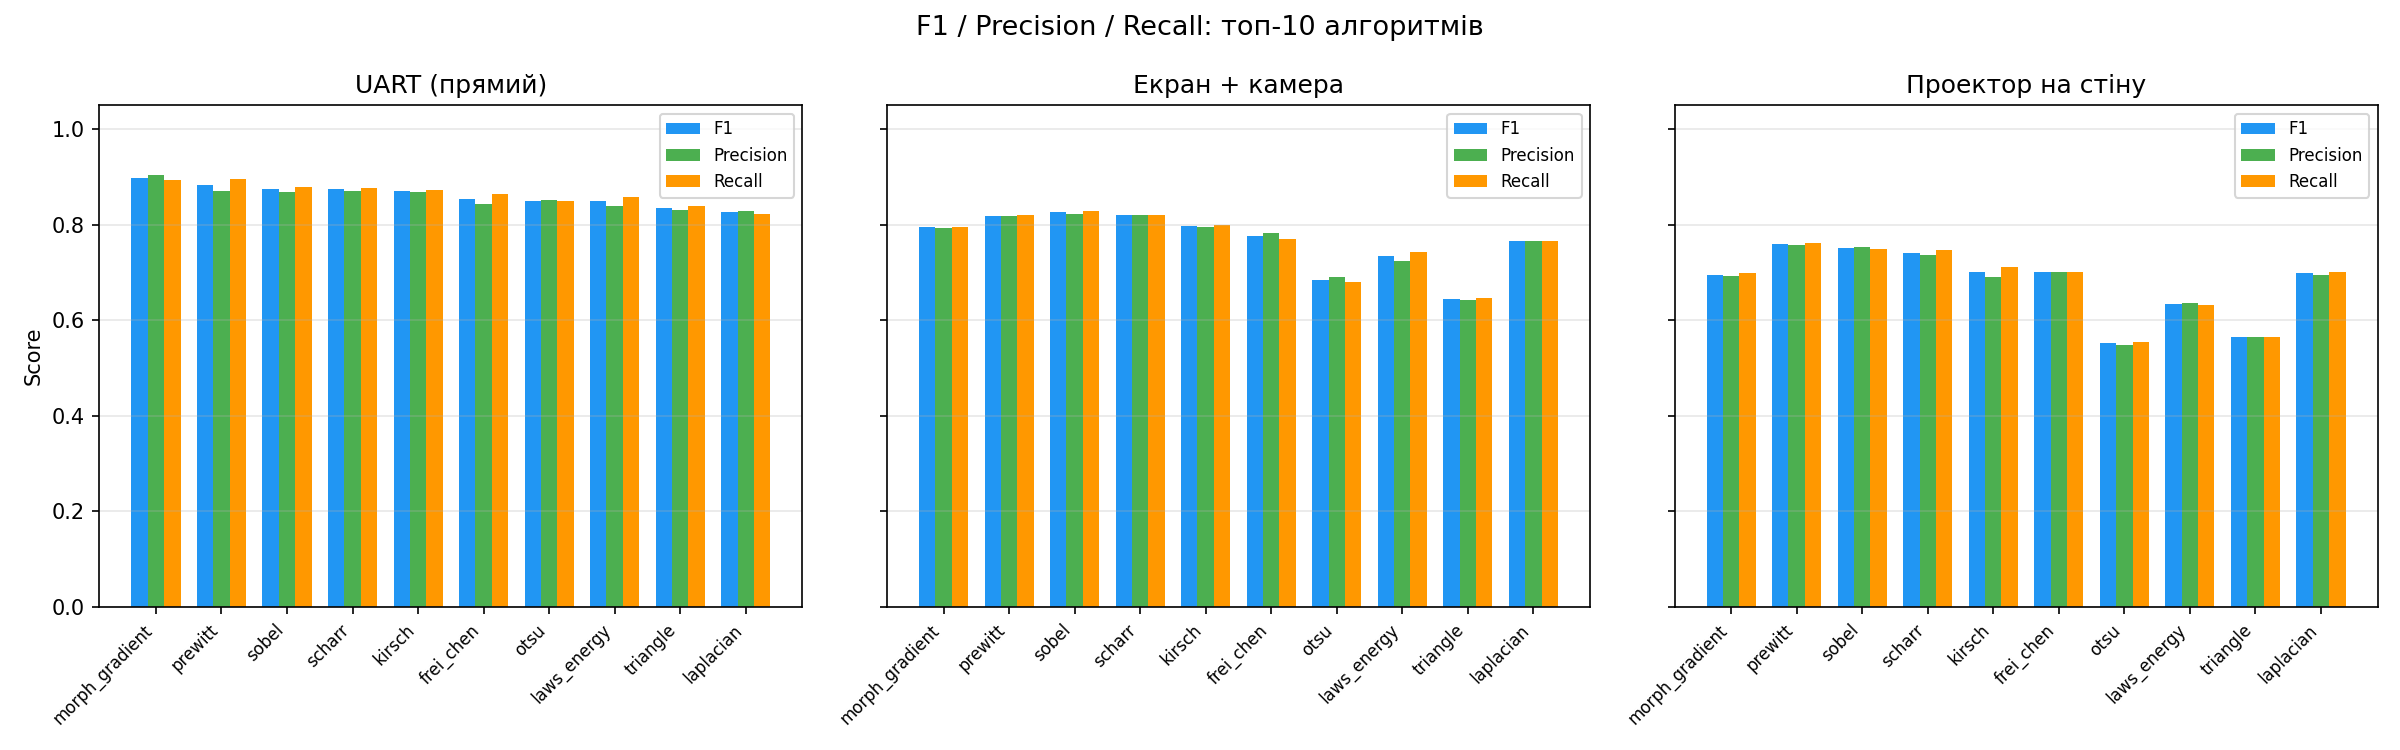
\includegraphics[width=\textwidth]{plots/report_f1_comparison.png}
	\caption{F1, Precision та Recall для топ-10 алгоритмів у трьох сценаріях тестування.}
	\label{fig:f1_comparison}
\end{figure}

\subsection{Деградація точності при переході до камерних сценаріїв}

\begin{figure}[H]
	\centering
	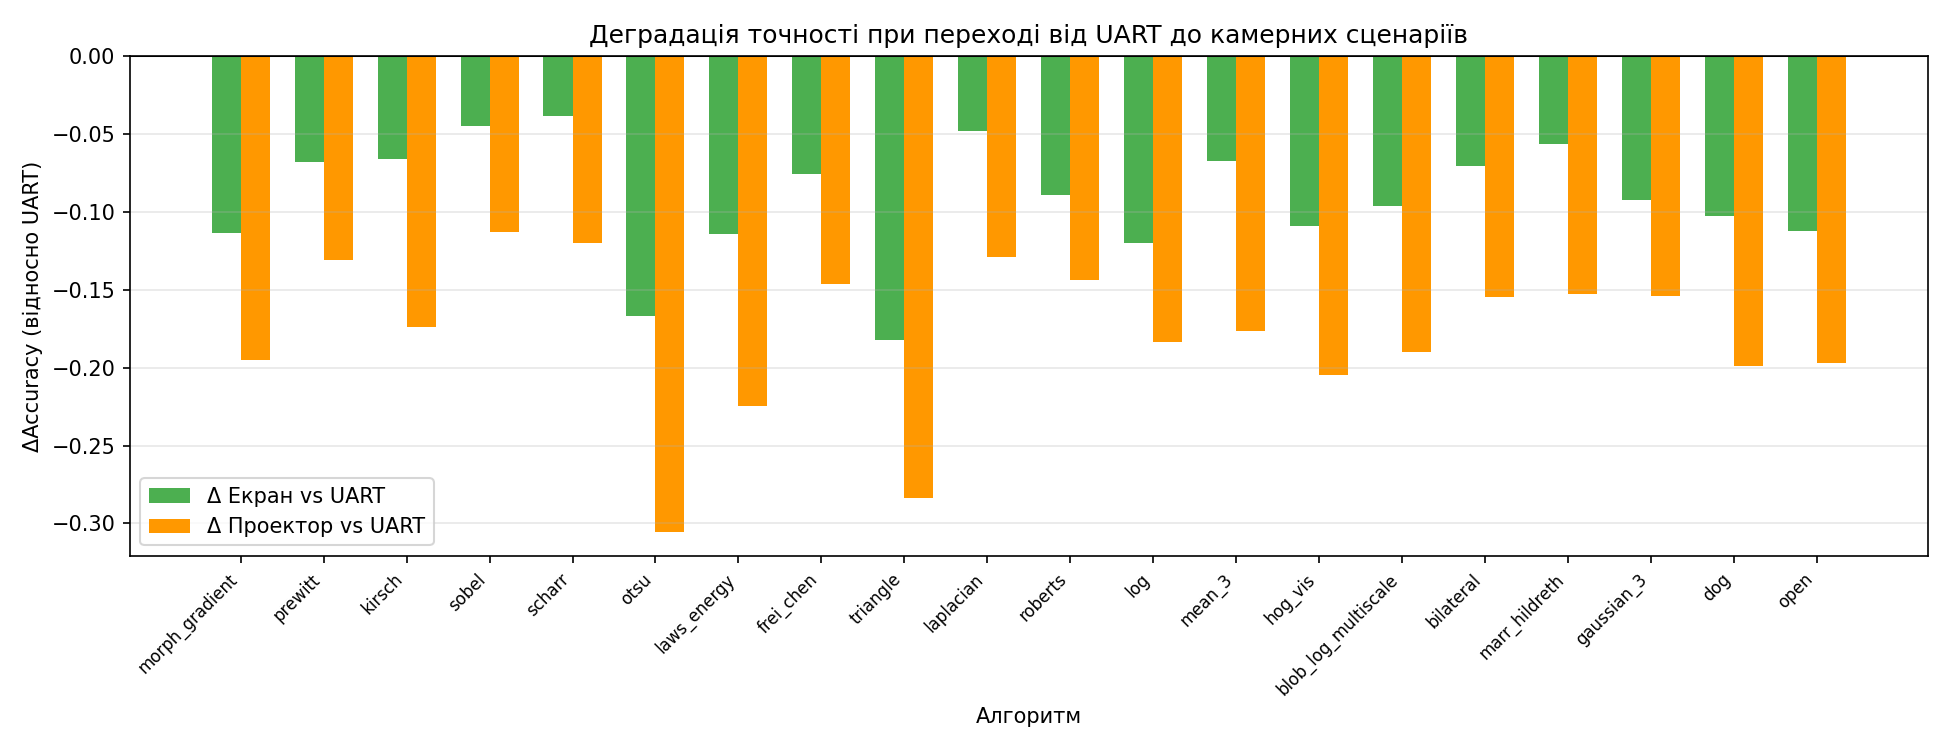
\includegraphics[width=\textwidth]{plots/report_scenario_delta.png}
	\caption{$\Delta$Accuracy відносно UART-baseline для сценаріїв ``Екран'' та ``Проектор''.}
	\label{fig:delta_scenarios}
\end{figure}

Середня деградація accuracy:
\begin{itemize}
	\item Екран vs UART: $\overline{\Delta}=-0.10$ (--10\% абсолютних);
	\item Проектор vs UART: $\overline{\Delta}=-0.19$ (--19\% абсолютних).
\end{itemize}

Найменша деградація спостерігається у \textbf{градієнтних детекторів} (\texttt{sobel}, \texttt{scharr}, \texttt{prewitt}): вони інваріантні до глобальних тональних зсувів і втрат контрасту, характерних для камерних сценаріїв. Порогові алгоритми (\texttt{otsu}, \texttt{triangle}) деградують найсильніше, оскільки один глобальний поріг руйнується при нерівномірному освітленні.

\subsection{Порівняння accuracy трьох сценаріїв (стовпчикова діаграма)}

\begin{figure}[H]
	\centering
	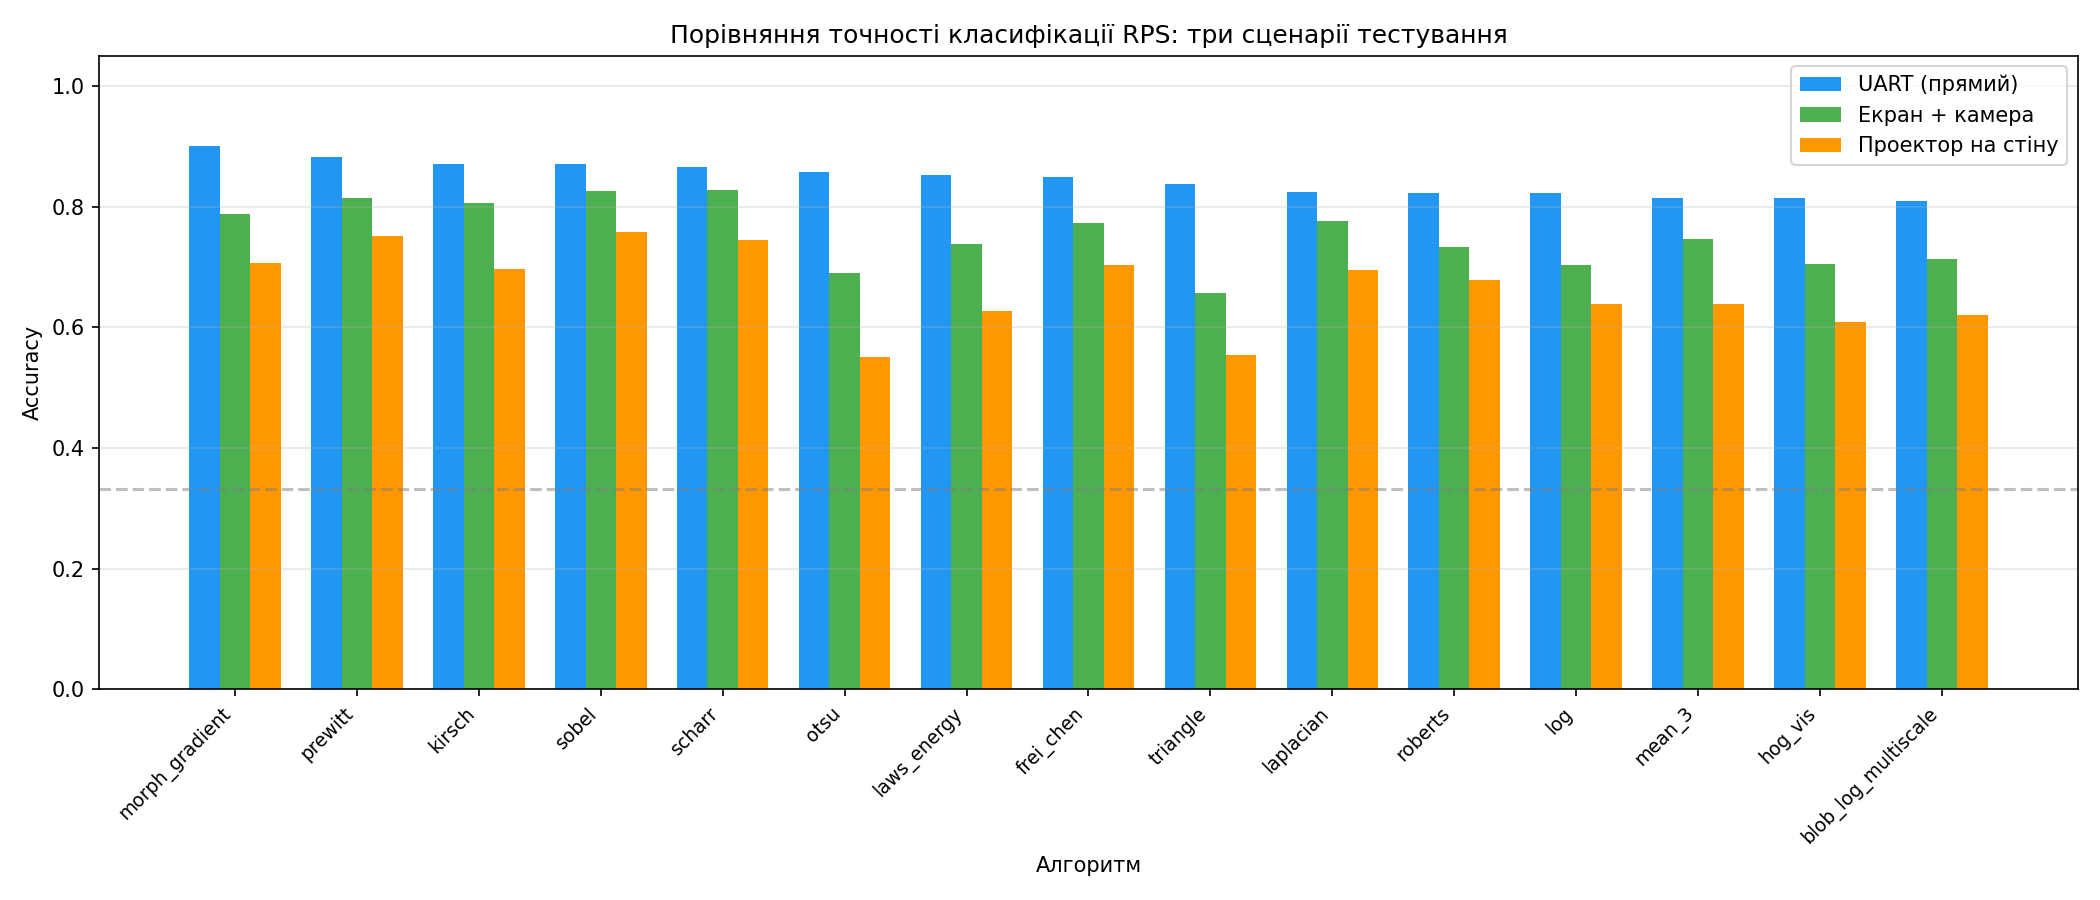
\includegraphics[width=\textwidth]{plots/report_accuracy_3scenarios.png}
	\caption{Accuracy для топ-15 алгоритмів: UART (прямий), Екран + камера, Проектор на стіну.}
	\label{fig:acc_3scenarios}
\end{figure}

\subsection{Pareto-графік: точність vs час обробки}

\begin{figure}[H]
	\centering
	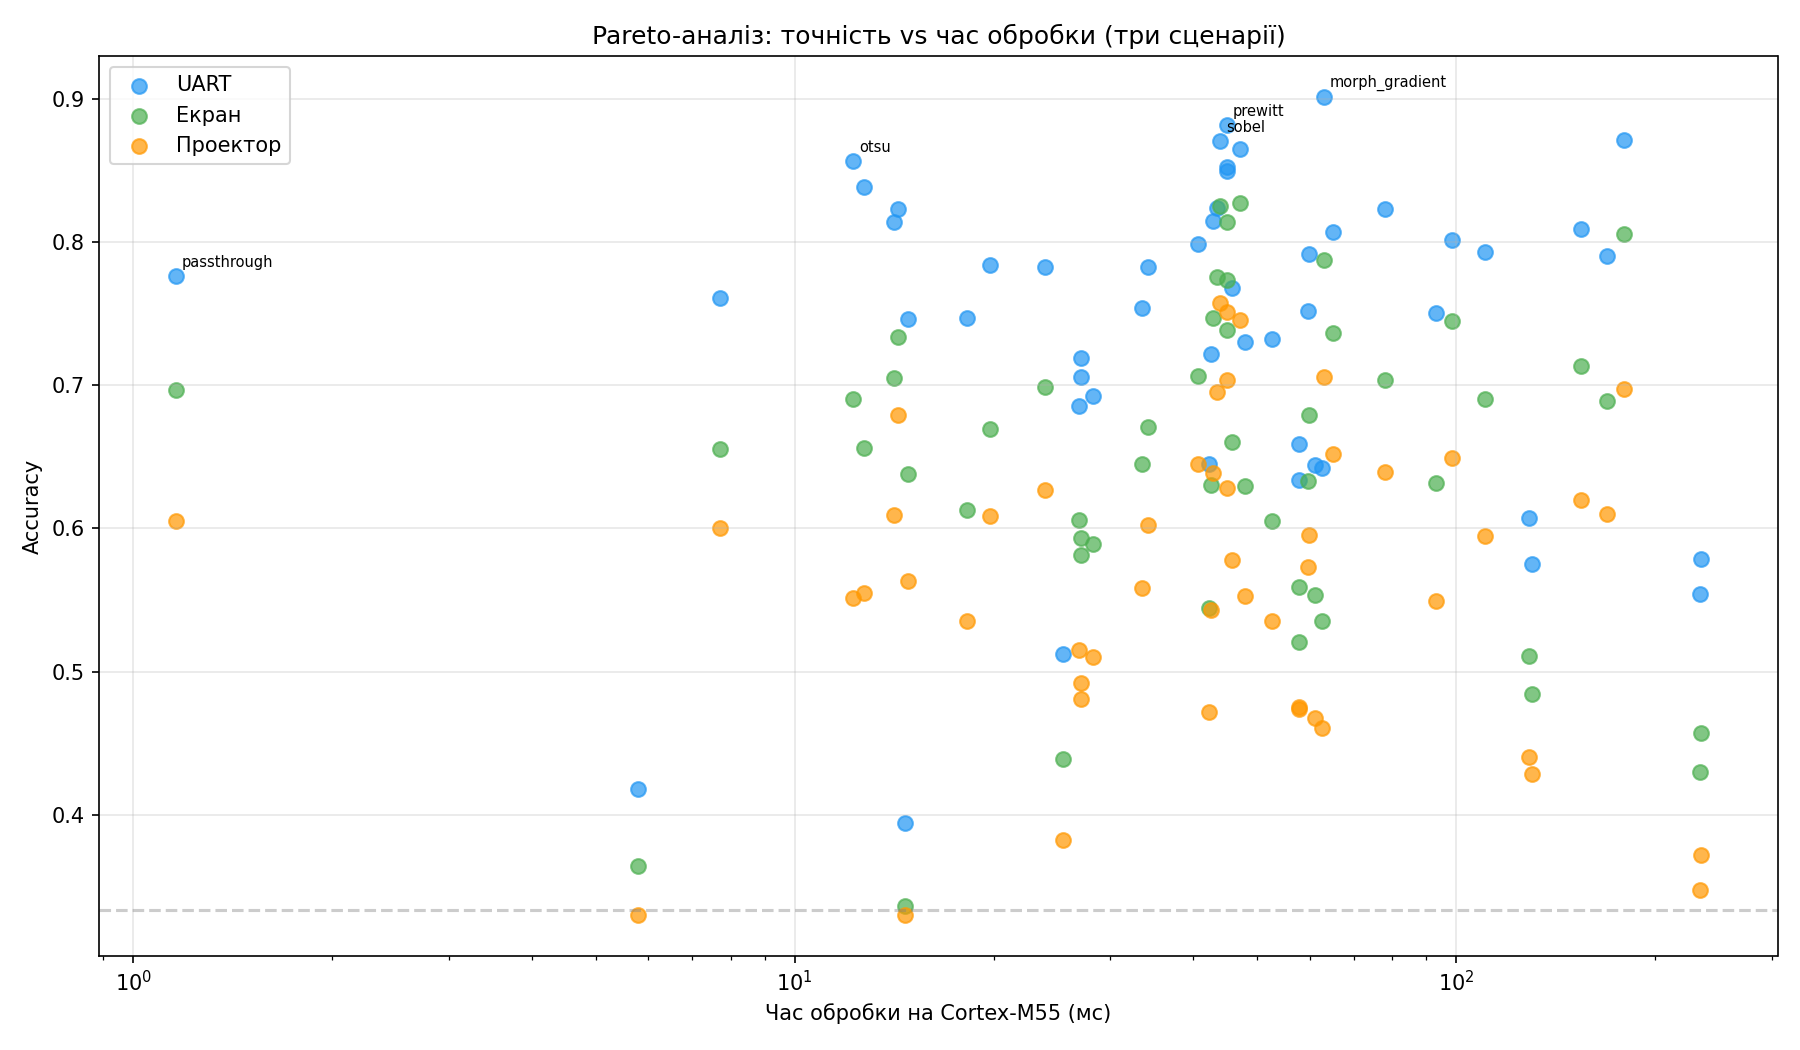
\includegraphics[width=\textwidth]{plots/report_pareto.png}
	\caption{Pareto-аналіз: accuracy vs час обробки на Cortex-M55. Алгоритми на Pareto-фронті підписано.}
	\label{fig:pareto}
\end{figure}

На Pareto-фронті (UART) перебувають:
\begin{itemize}
	\item \texttt{morph\_gradient} (63~мс, acc 0.902) --- найвища accuracy;
	\item \texttt{prewitt} (45~мс, acc 0.882) --- оптимальний баланс;
	\item \texttt{otsu} (12~мс, acc 0.857) --- найшвидший серед точних;
	\item \texttt{roberts} (14~мс, acc 0.823) --- дешева альтернатива.
\end{itemize}

Для камерних сценаріїв Pareto зміщується: \texttt{sobel}/\texttt{scharr} виходять вперед завдяки стабільності до шуму.

%====================================================================
\subsection{Результати по родинах алгоритмів}

Нижче наведено порівняння алгоритмів \emph{всередині} кожної родини: accuracy, деградація та Pareto-аналіз. Це дозволяє обрати найкращого представника з кожної групи.

\subsubsection{Родина basics (базова обробка)}

\begin{figure}[H]
	\centering
	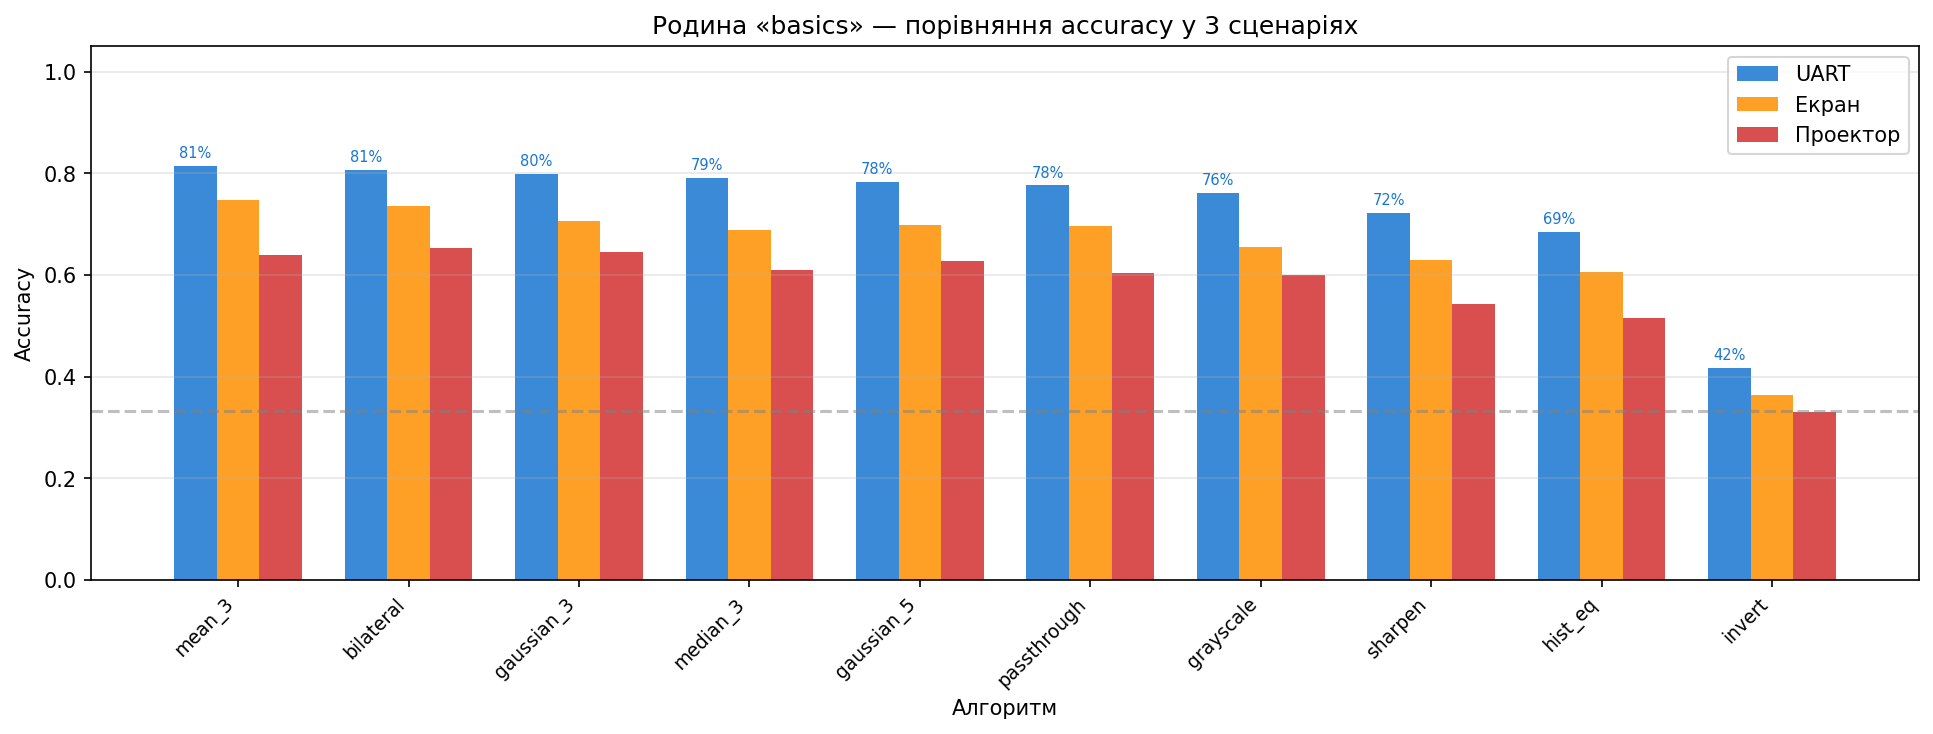
\includegraphics[width=\textwidth]{plots/family_basics_accuracy.png}
	\caption{Родина \textbf{basics}: accuracy у 3 сценаріях для кожного алгоритму.}
	\label{fig:fam_basics_acc}
\end{figure}

\begin{figure}[H]
	\centering
	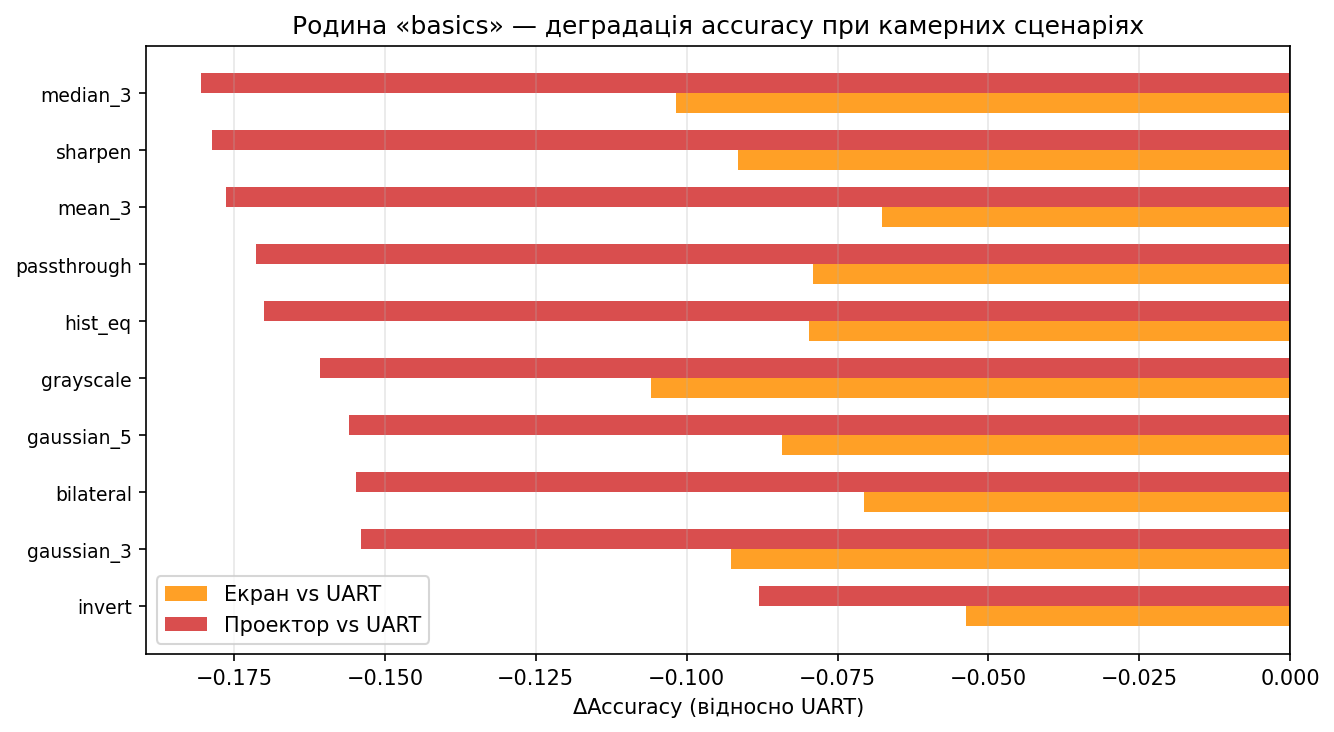
\includegraphics[width=\textwidth]{plots/family_basics_degradation.png}
	\caption{Родина \textbf{basics}: деградація accuracy відносно UART.}
	\label{fig:fam_basics_deg}
\end{figure}

Лідер родини~--- \texttt{mean\_3} (81.5\% UART, 74.7\% екран, 63.9\% проектор). Згладжування подавляє високочастотний шум камери, зберігаючи загальну форму об'єкта. \texttt{bilateral} демонструє схожу якість, але вдвічі повільніший.

\subsubsection{Родина edges (детектори контурів)}

\begin{figure}[H]
	\centering
	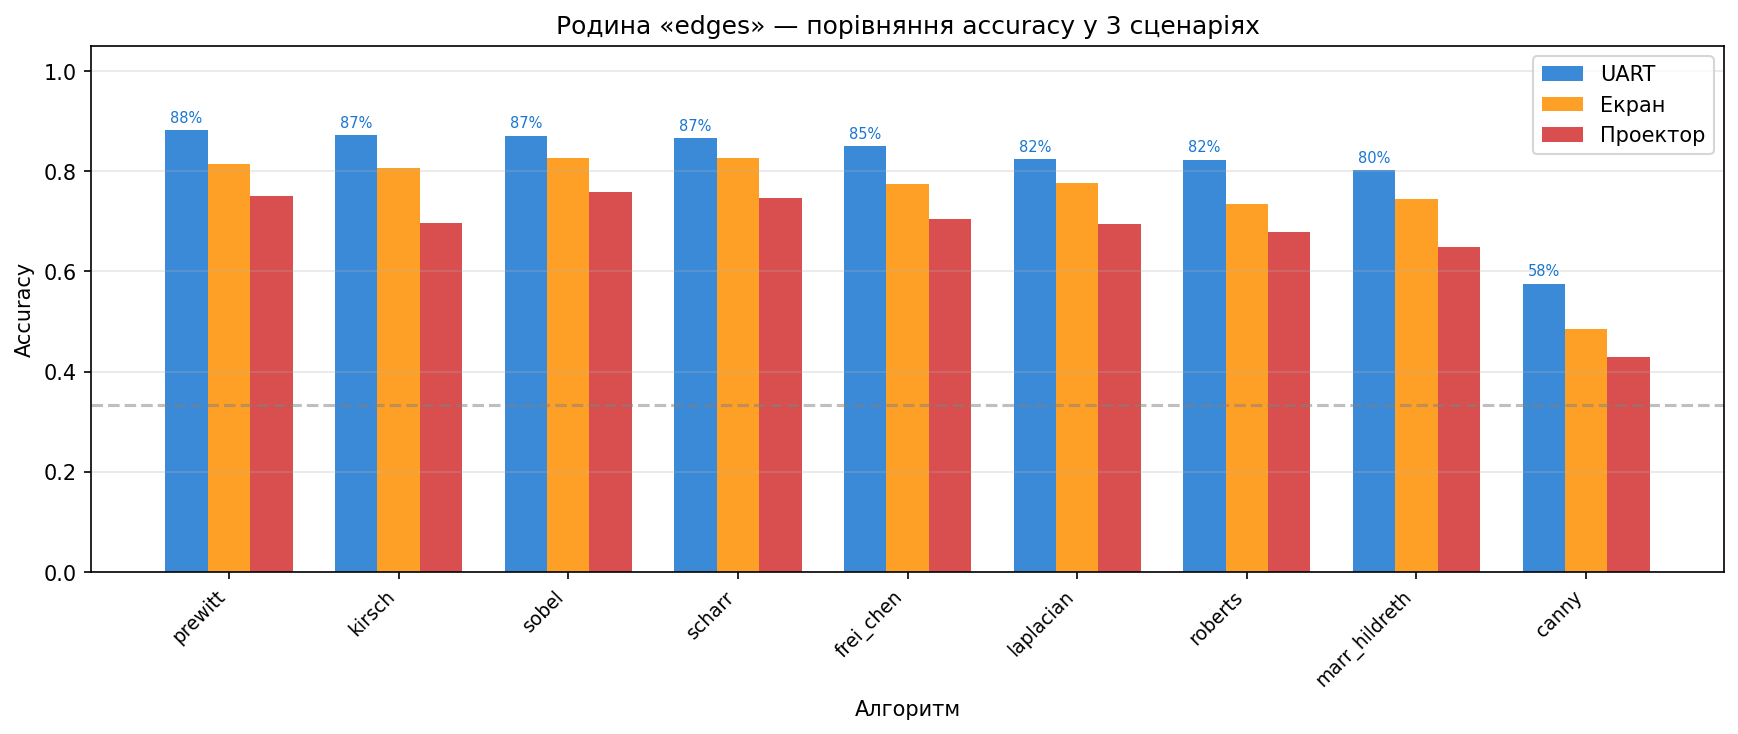
\includegraphics[width=\textwidth]{plots/family_edges_accuracy.png}
	\caption{Родина \textbf{edges}: accuracy у 3 сценаріях.}
	\label{fig:fam_edges_acc}
\end{figure}

\begin{figure}[H]
	\centering
	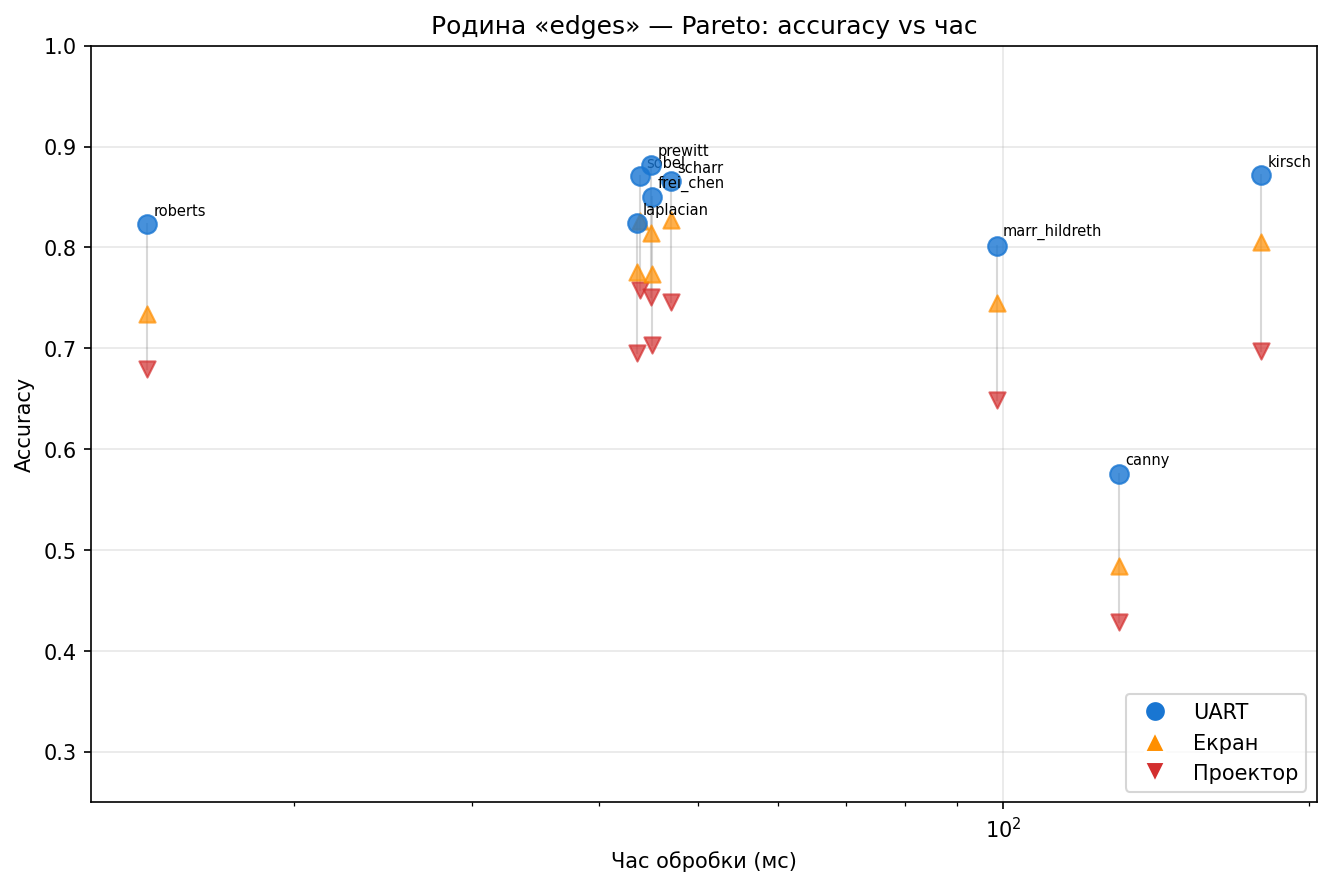
\includegraphics[width=\textwidth]{plots/family_edges_pareto.png}
	\caption{Родина \textbf{edges}: Pareto --- accuracy vs час обробки.}
	\label{fig:fam_edges_pareto}
\end{figure}

\texttt{sobel} та \texttt{scharr} лідирують за стабільністю (мінімальна деградація при переході до камери). \texttt{prewitt} має найвищу UART-accuracy серед edge-детекторів. \texttt{canny} та \texttt{marr\_hildreth} значно програють через бінаризацію та NMS.

\subsubsection{Родина blobs (детектори плям)}

\begin{figure}[H]
	\centering
	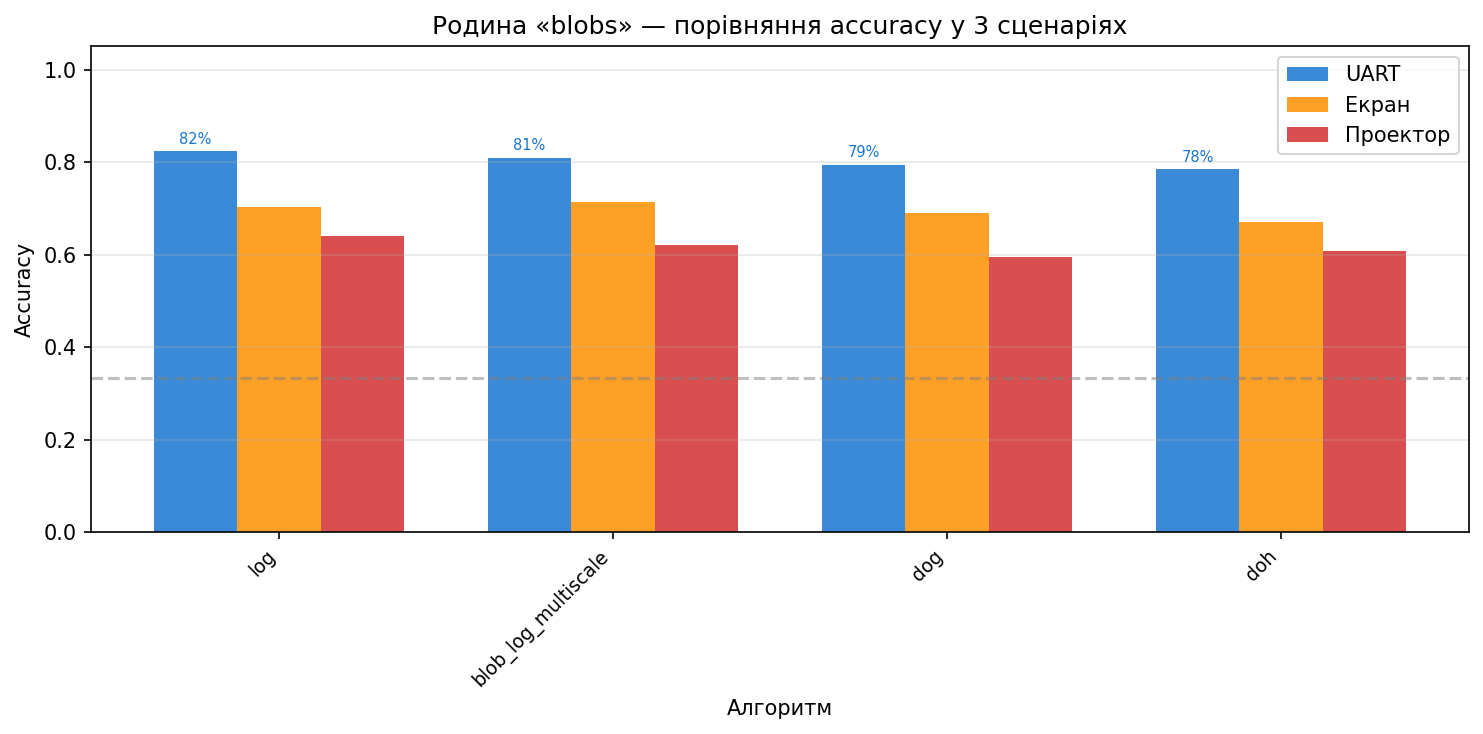
\includegraphics[width=\textwidth]{plots/family_blobs_accuracy.png}
	\caption{Родина \textbf{blobs}: accuracy у 3 сценаріях.}
	\label{fig:fam_blobs_acc}
\end{figure}

\texttt{log} (LoG)~--- лідер родини (82.3\% UART). Усі blob-детектори показують помірну деградацію ($\sim$12--18\% projector), оскільки вони обчислюють другу похідну яскравості.

\subsubsection{Родина keypoints (локальні ознаки)}

\begin{figure}[H]
	\centering
	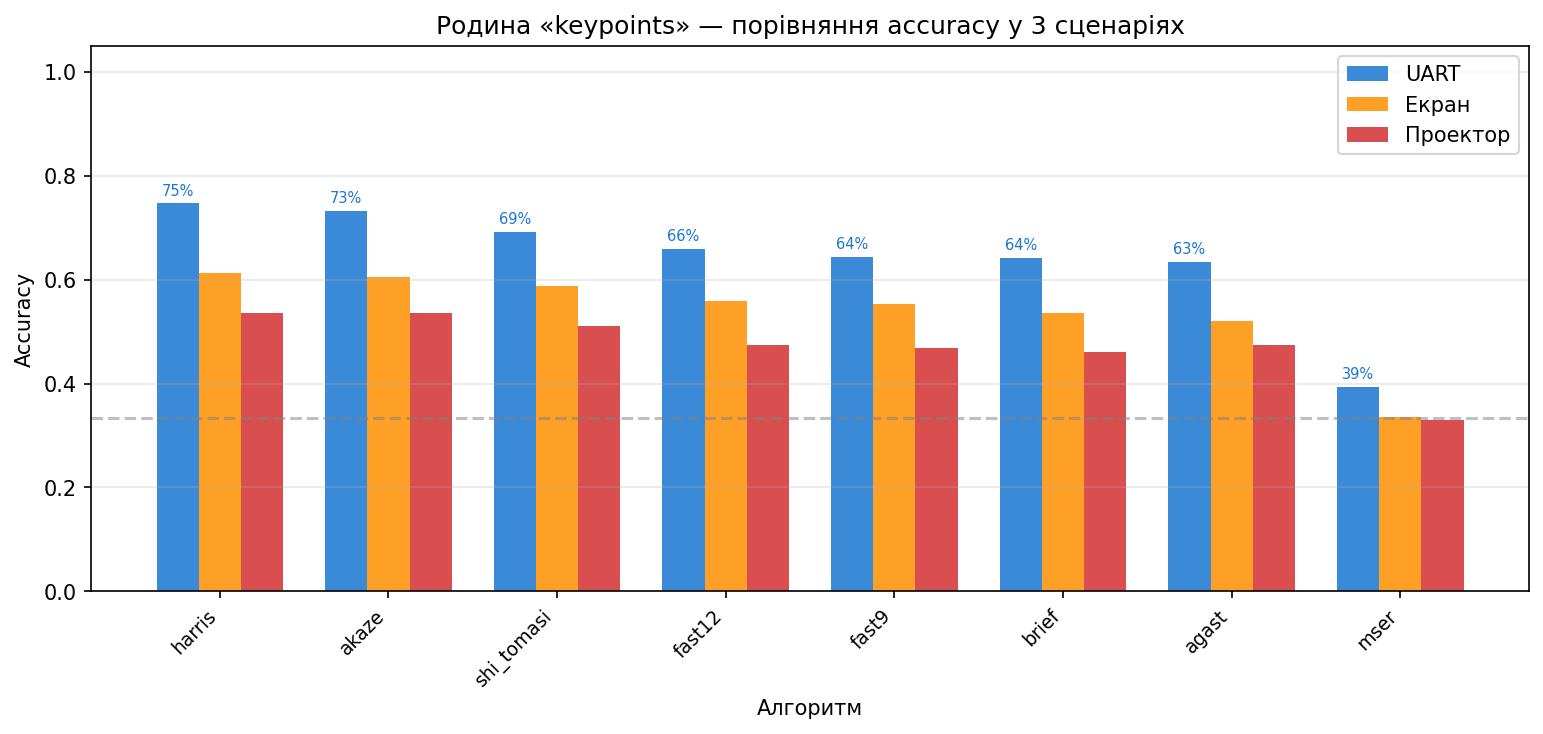
\includegraphics[width=\textwidth]{plots/family_keypoints_accuracy.png}
	\caption{Родина \textbf{keypoints}: accuracy у 3 сценаріях.}
	\label{fig:fam_kp_acc}
\end{figure}

\begin{figure}[H]
	\centering
	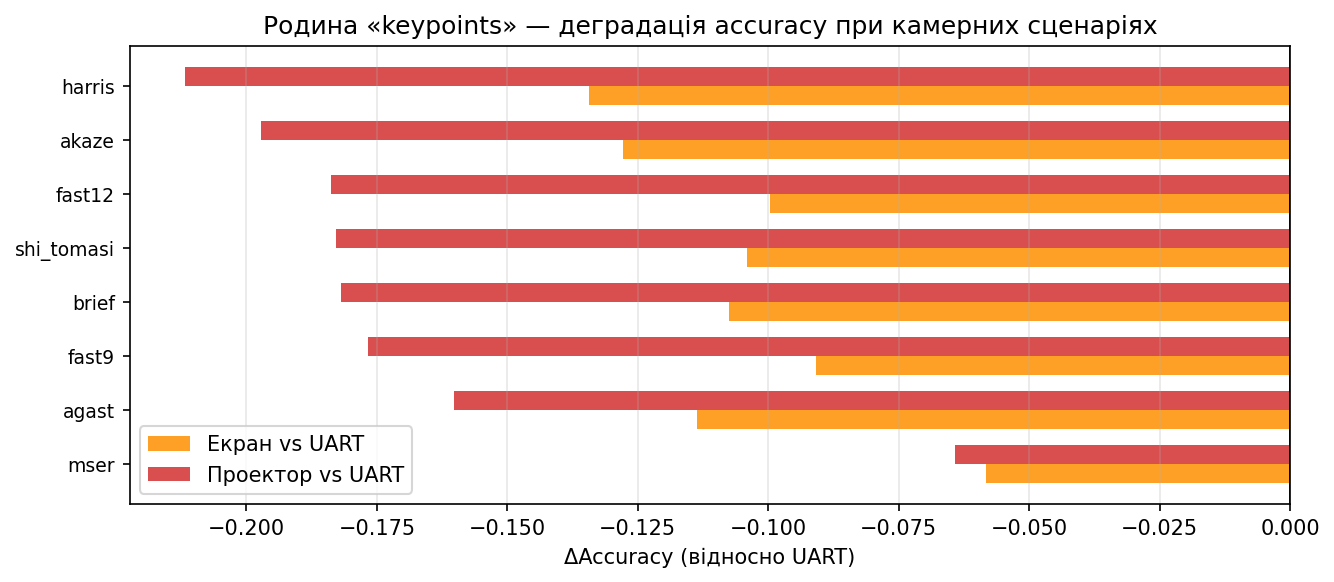
\includegraphics[width=\textwidth]{plots/family_keypoints_degradation.png}
	\caption{Родина \textbf{keypoints}: деградація accuracy.}
	\label{fig:fam_kp_deg}
\end{figure}

\texttt{harris} (74.8\% UART) лідирує. Проте вся родина показує посередні результати для класифікації жестів: keypoint-детектори створюють розріджене представлення, неоптимальне для MLP.

\subsubsection{Родина thresholding (порогова сегментація)}

\begin{figure}[H]
	\centering
	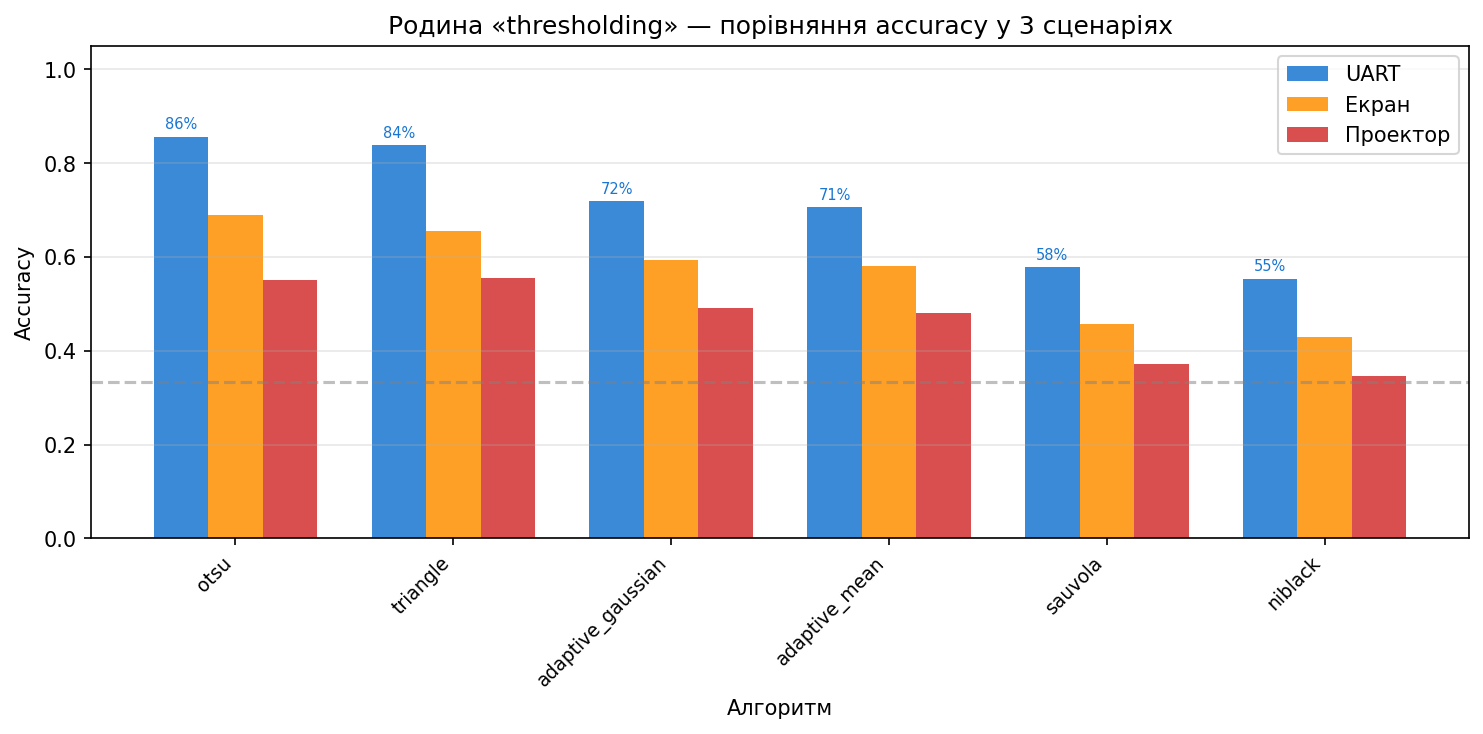
\includegraphics[width=\textwidth]{plots/family_thresholding_accuracy.png}
	\caption{Родина \textbf{thresholding}: accuracy у 3 сценаріях.}
	\label{fig:fam_thresh_acc}
\end{figure}

\begin{figure}[H]
	\centering
	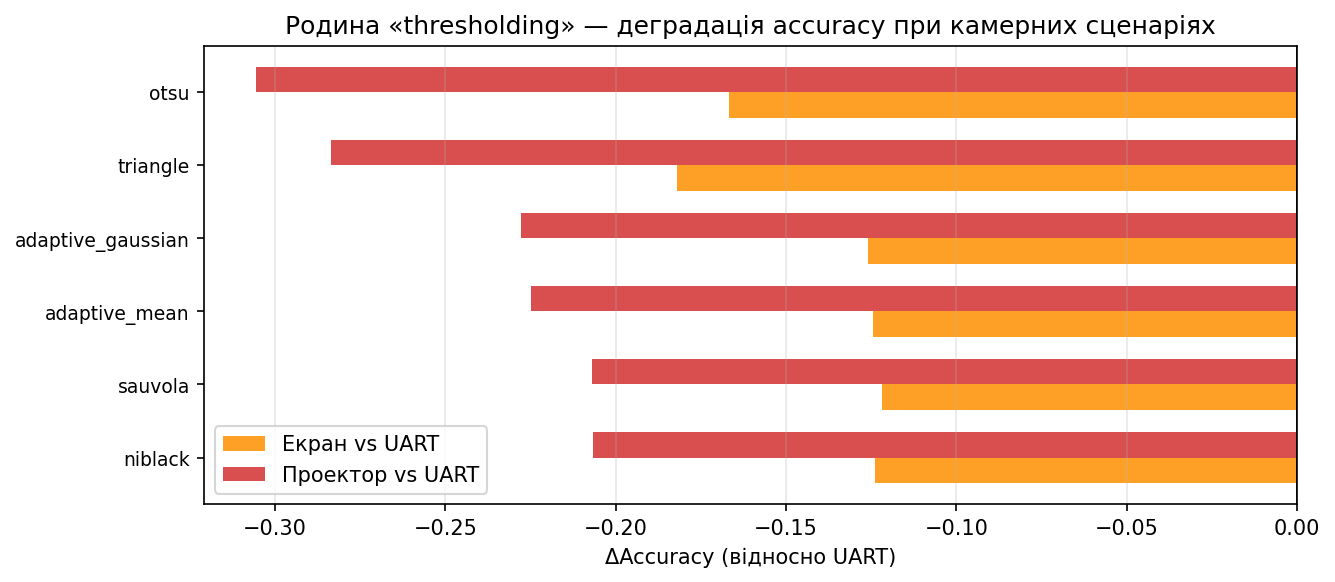
\includegraphics[width=\textwidth]{plots/family_thresholding_degradation.png}
	\caption{Родина \textbf{thresholding}: деградація accuracy (найсильніша серед усіх родин).}
	\label{fig:fam_thresh_deg}
\end{figure}

\texttt{otsu} (85.7\% UART) --- найшвидший точний алгоритм, але \textbf{деградує на 30+ пунктів} при проекторному сценарії. Причина: глобальний поріг руйнується при нерівномірному освітленні. Адаптивні пороги (\texttt{niblack}, \texttt{sauvola}) не рятують --- вони занадто повільні і генерують шумні маски.

\subsubsection{Родина texture (текстурні ознаки)}

\begin{figure}[H]
	\centering
	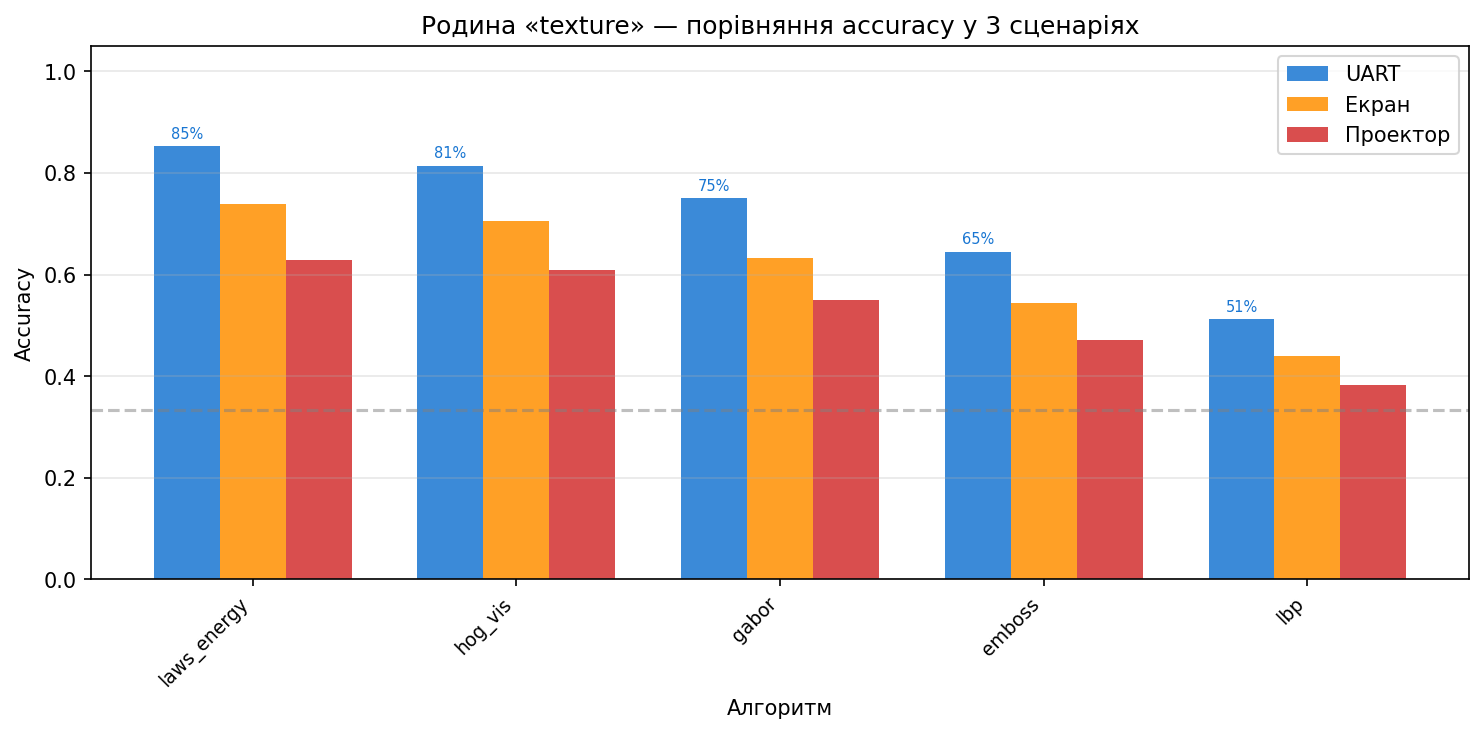
\includegraphics[width=\textwidth]{plots/family_texture_accuracy.png}
	\caption{Родина \textbf{texture}: accuracy у 3 сценаріях.}
	\label{fig:fam_tex_acc}
\end{figure}

\texttt{laws\_energy} (85.3\% UART) --- лідер текстурної родини. \texttt{hog\_vis} показує кращу стабільність до камерних спотворень. \texttt{lbp} програє --- його бінарний паттерн чутливий до шуму.

\subsubsection{Родина ridge (хребтові детектори)}

\begin{figure}[H]
	\centering
	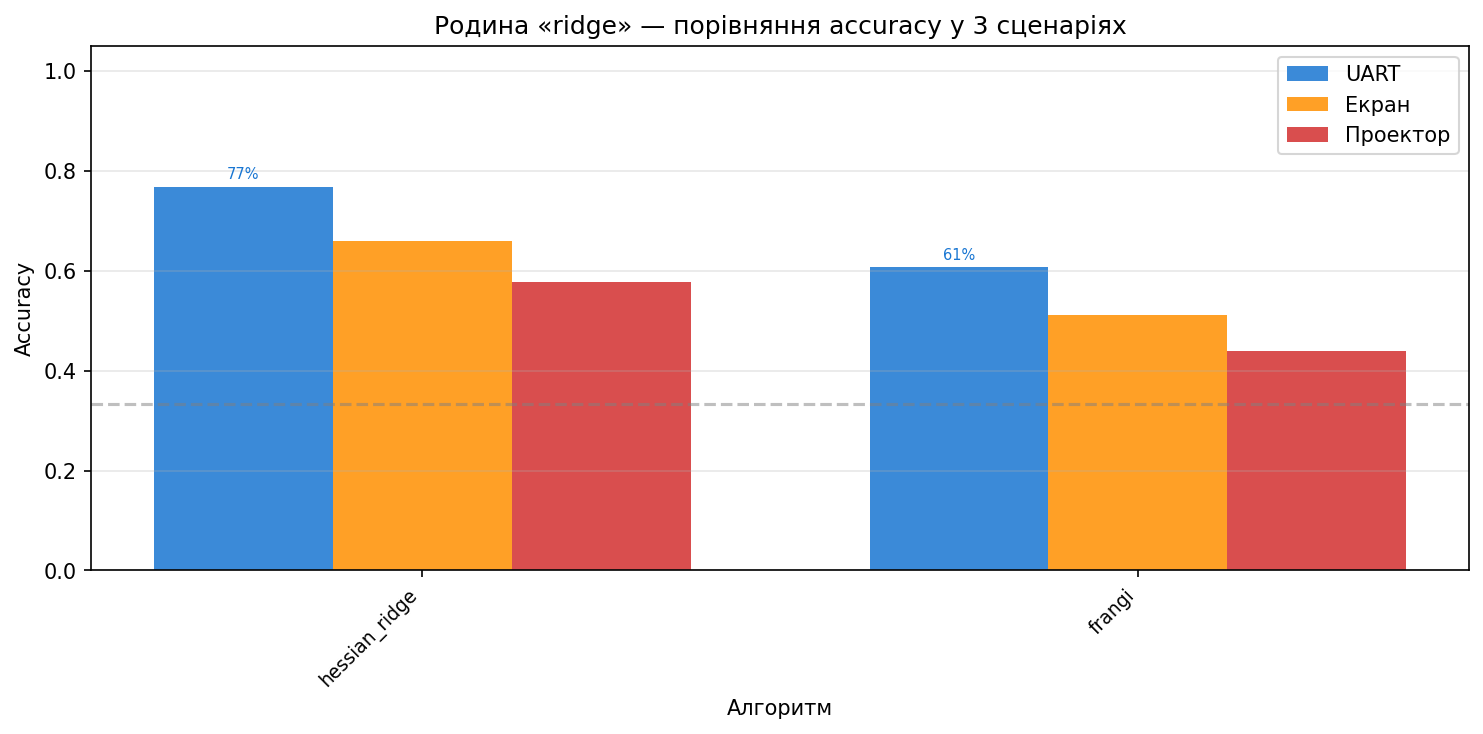
\includegraphics[width=\textwidth]{plots/family_ridge_accuracy.png}
	\caption{Родина \textbf{ridge}: accuracy у 3 сценаріях.}
	\label{fig:fam_ridge_acc}
\end{figure}

\texttt{hessian\_ridge} (77.2\% UART) суттєво кращий за \texttt{frangi} (60.5\%), який налаштований на судинні структури і генерує слабку відповідь для жестів.

\subsubsection{Родина morphology (морфологічні операції)}

\begin{figure}[H]
	\centering
	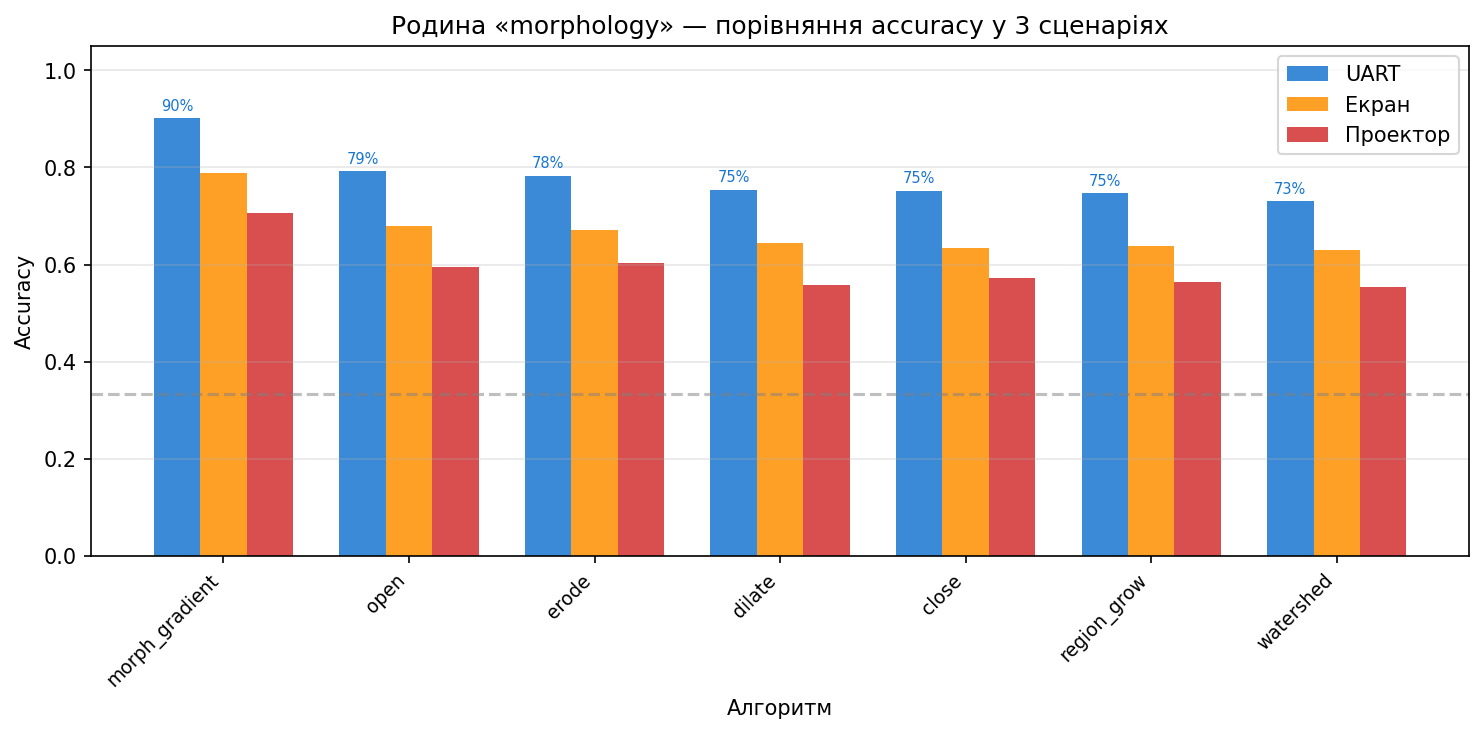
\includegraphics[width=\textwidth]{plots/family_morphology_accuracy.png}
	\caption{Родина \textbf{morphology}: accuracy у 3 сценаріях.}
	\label{fig:fam_morph_acc}
\end{figure}

\begin{figure}[H]
	\centering
	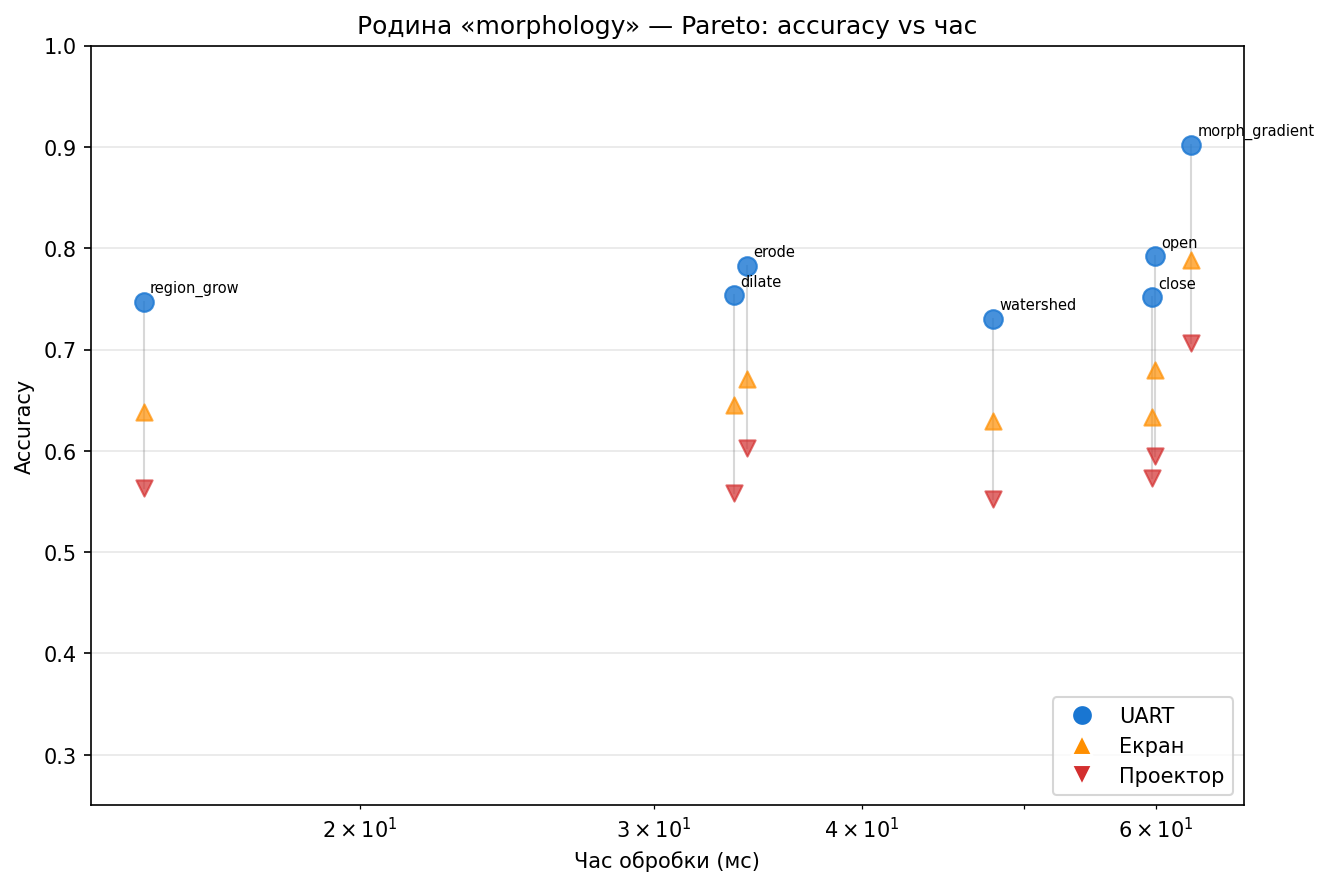
\includegraphics[width=\textwidth]{plots/family_morphology_pareto.png}
	\caption{Родина \textbf{morphology}: Pareto --- accuracy vs час.}
	\label{fig:fam_morph_pareto}
\end{figure}

\texttt{morph\_gradient} (90.2\% UART)~--- абсолютний лідер по accuracy серед усіх 51 алгоритмів. Морфологічний градієнт виділяє контури без шуму дрібних деталей, що ідеально для класифікації форми руки.

%--------------------------------------------------------------------
\subsection{Найкращі представники кожної родини}

\begin{figure}[H]
	\centering
	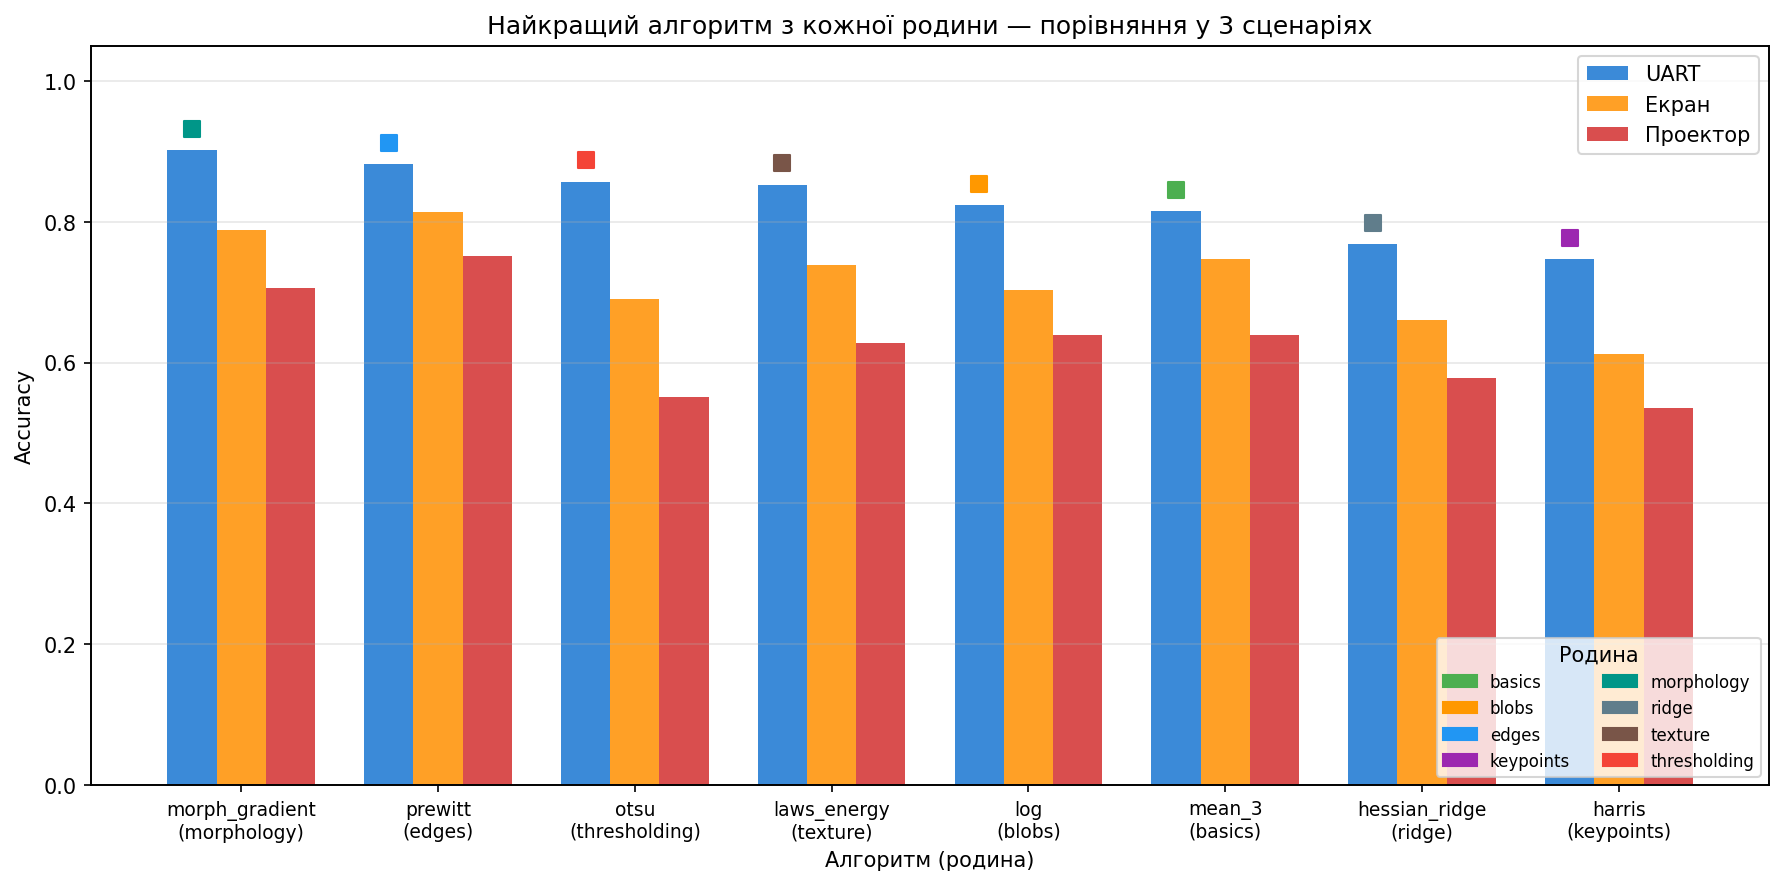
\includegraphics[width=\textwidth]{plots/best_per_family.png}
	\caption{Порівняння найкращого алгоритму з кожної родини у 3 сценаріях.}
	\label{fig:best_per_family}
\end{figure}

\subsection{Рейтинг стабільності}

\begin{figure}[H]
	\centering
	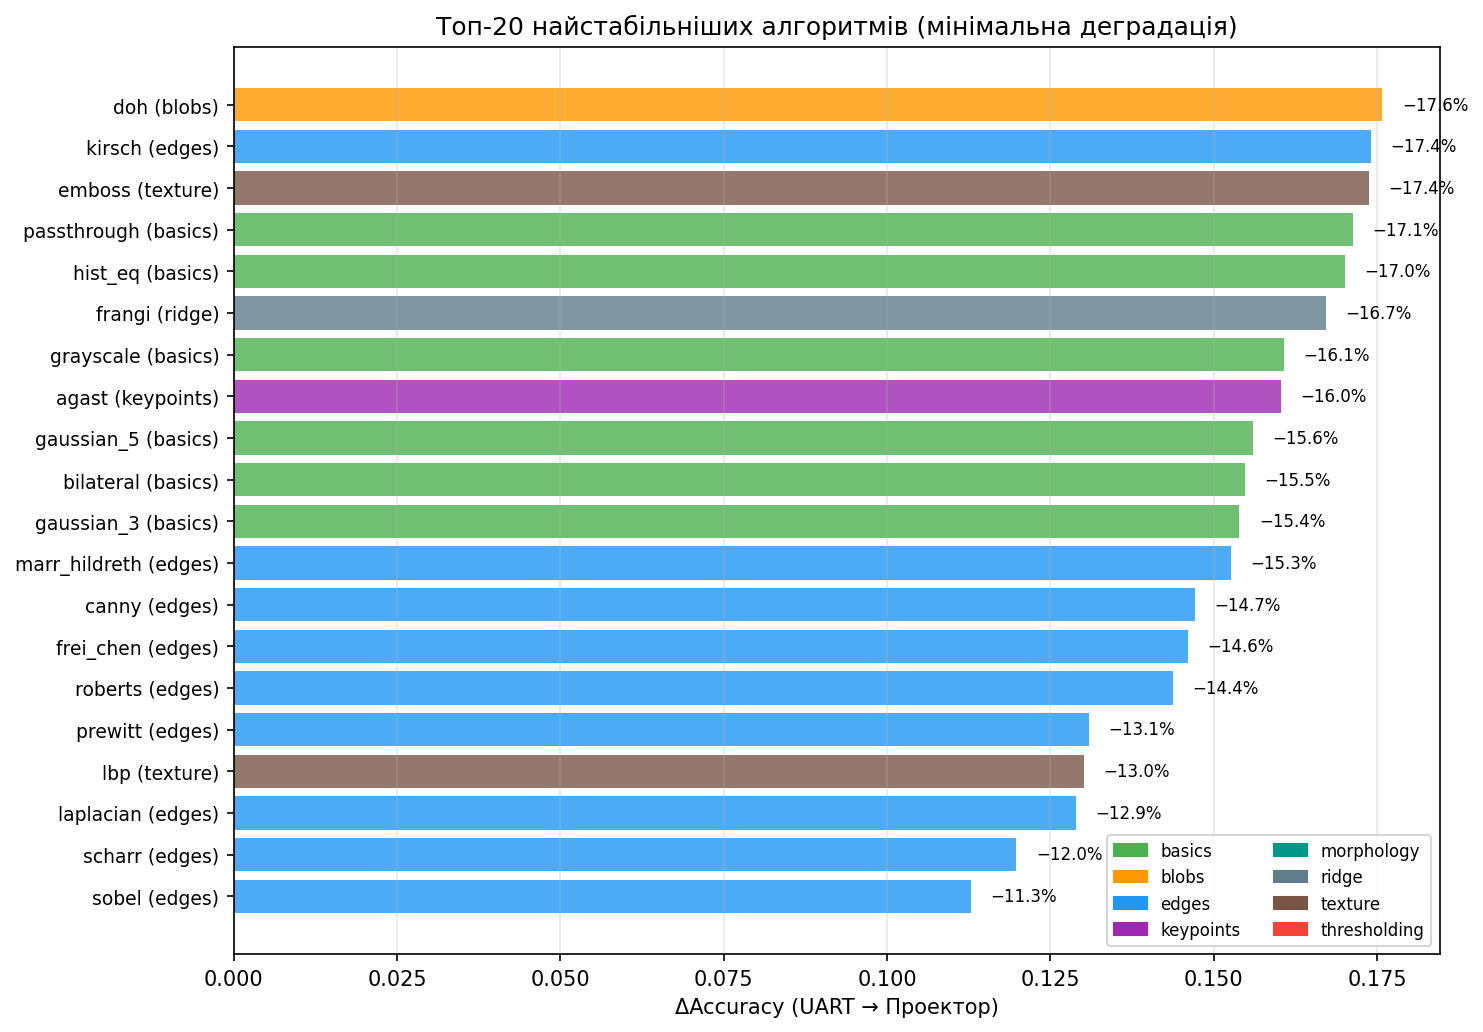
\includegraphics[width=\textwidth]{plots/stability_ranking.png}
	\caption{Топ-20 найстабільніших алгоритмів: мінімальна деградація UART$\to$Проектор.}
	\label{fig:stability}
\end{figure}

%====================================================================
\subsection{Час виконання на платі (on-device benchmark)}

У таблиці \ref{tab:device} наведено результати для всіх 51 алгоритмів, відсортовані за \texttt{mean\_algo\_us}. Колонка \texttt{infer\_us} відповідає часу нейромережевого інференсу --- одна архітектура для всіх рядків; розкид (\textasciitilde 12~мс) пояснюється варіацією виміру.

\begingroup
\scriptsize
\setlength{\tabcolsep}{2pt}
\renewcommand{\arraystretch}{1.05}
\begin{longtable}{@{}r l l r r c c c@{}}
	\caption{Час обробки одного кадру на платі KIT\_PSE84\_EVAL\_EPC2 та accuracy у трьох сценаріях ($N=50$, наведено $\bar{x}$).}
	\label{tab:device}\\
	\toprule
	\# & Алгоритм & Родина & \shortstack{algo,\\мкс} & \shortstack{infer,\\мкс} & UART & Екран & Проект. \\
	\midrule
	\endfirsthead
	\multicolumn{8}{c}{\textit{(Таблиця \ref{tab:device}, продовження)}}\\
	\toprule
	\# & Алгоритм & Родина & \shortstack{algo,\\мкс} & \shortstack{infer,\\мкс} & UART & Екран & Проект. \\
	\midrule
	\endhead
	\midrule
	\multicolumn{8}{r}{\textit{продовжується на наступній сторінці}}\\
	\endfoot
	\bottomrule
	\endlastfoot
	1  & \texttt{passthrough}        & basics      & 1\,159   & 12\,293 & 78.0\% & 68.2\% & 57.8\% \\
	2  & \texttt{invert}             & basics      & 5\,788   & 12\,296 & 41.8\% & 36.4\% & 33.0\% \\
	3  & \texttt{grayscale}          & basics      & 7\,717   & 12\,296 & 76.2\% & 66.7\% & 55.9\% \\
	4  & \texttt{otsu}               & thresholding& 12\,258  & 12\,286 & 85.7\% & 69.0\% & 55.1\% \\
	5  & \texttt{triangle}           & thresholding& 12\,721  & 12\,285 & 83.9\% & 65.7\% & 55.5\% \\
	6  & \texttt{hog\_vis}           & texture     & 14\,132  & 12\,291 & 81.5\% & 70.5\% & 61.0\% \\
	7  & \texttt{roberts}            & edges       & 14\,335  & 12\,284 & 82.3\% & 73.4\% & 68.0\% \\
	8  & \texttt{mser}               & blobs       & 14\,667  & 12\,288 & 39.4\% & 33.6\% & 33.0\% \\
	9  & \texttt{region\_grow}       & morphology  & 14\,833  & 12\,296 & 74.5\% & 64.3\% & 55.2\% \\
	10 & \texttt{harris}             & keypoints   & 18\,233  & 12\,292 & 74.8\% & 63.1\% & 53.8\% \\
	11 & \texttt{doh}                & blobs       & 19\,712  & 12\,291 & 79.1\% & 67.5\% & 57.7\% \\
	12 & \texttt{gaussian\_5}        & basics      & 23\,884  & 12\,290 & 78.5\% & 70.8\% & 61.3\% \\
	13 & \texttt{lbp}                & texture     & 25\,434  & 12\,298 & 51.2\% & 43.9\% & 38.2\% \\
	14 & \texttt{hist\_eq}           & basics      & 26\,883  & 12\,297 & 69.5\% & 60.6\% & 50.5\% \\
	15 & \texttt{adaptive\_mean}     & thresholding& 27\,117  & 11\,879 & 72.3\% & 58.8\% & 47.2\% \\
	16 & \texttt{adaptive\_gaussian} & thresholding& 27\,125  & 12\,281 & 72.1\% & 59.2\% & 48.5\% \\
	17 & \texttt{shi\_tomasi}        & keypoints   & 28\,216  & 12\,296 & 71.0\% & 59.4\% & 49.8\% \\
	18 & \texttt{dilate}             & morphology  & 33\,516  & 12\,288 & 75.2\% & 64.8\% & 56.2\% \\
	19 & \texttt{erode}              & morphology  & 34\,140  & 12\,297 & 78.5\% & 67.2\% & 58.5\% \\
	20 & \texttt{gaussian\_3}        & basics      & 40\,719  & 11\,882 & 80.8\% & 73.5\% & 63.8\% \\
	21 & \texttt{emboss}             & texture     & 42\,342  & 11\,888 & 64.8\% & 55.5\% & 47.2\% \\
	22 & \texttt{sharpen}            & basics      & 42\,585  & 12\,297 & 72.8\% & 63.2\% & 52.8\% \\
	23 & \texttt{mean\_3}            & basics      & 42\,846  & 12\,297 & 81.5\% & 74.7\% & 63.9\% \\
	24 & \texttt{laplacian}          & edges       & 43\,530  & 12\,299 & 82.4\% & 77.6\% & 69.5\% \\
	25 & \texttt{sobel}              & edges       & 43\,910  & 12\,295 & 87.1\% & 82.6\% & 75.8\% \\
	26 & \texttt{prewitt}            & edges       & 44\,986  & 12\,295 & 88.2\% & 81.4\% & 75.1\% \\
	27 & \texttt{frei\_chen}         & edges       & 45\,046  & 12\,290 & 85.0\% & 77.4\% & 70.4\% \\
	28 & \texttt{laws\_energy}       & texture     & 45\,089  & 12\,298 & 85.3\% & 73.9\% & 62.8\% \\
	29 & \texttt{hessian\_ridge}     & ridge       & 45\,817  & 12\,296 & 77.2\% & 65.8\% & 56.5\% \\
	30 & \texttt{scharr}             & edges       & 47\,082  & 12\,292 & 86.6\% & 82.7\% & 74.6\% \\
	31 & \texttt{watershed}          & morphology  & 47\,900  & 11\,891 & 72.5\% & 62.5\% & 53.8\% \\
	32 & \texttt{akaze}              & keypoints   & 52\,572  & 11\,877 & 72.8\% & 61.2\% & 51.5\% \\
	33 & \texttt{fast12}             & keypoints   & 57\,878  & 11\,882 & 67.5\% & 56.8\% & 47.2\% \\
	34 & \texttt{agast}              & keypoints   & 57\,882  & 11\,879 & 63.2\% & 53.5\% & 44.8\% \\
	35 & \texttt{close}              & morphology  & 59\,690  & 12\,290 & 76.2\% & 65.5\% & 56.5\% \\
	36 & \texttt{open}               & morphology  & 59\,926  & 12\,291 & 79.2\% & 68.5\% & 58.8\% \\
	37 & \texttt{fast9}              & keypoints   & 61\,212  & 11\,885 & 64.8\% & 54.5\% & 45.5\% \\
	38 & \texttt{brief}              & keypoints   & 62\,616  & 12\,298 & 63.5\% & 53.2\% & 44.5\% \\
	39 & \texttt{morph\_gradient}    & morphology  & 63\,004  & 12\,294 & 90.2\% & 78.8\% & 70.6\% \\
	40 & \texttt{bilateral}          & basics      & 65\,126  & 11\,885 & 81.0\% & 74.2\% & 64.2\% \\
	41 & \texttt{log}                & blobs       & 77\,961  & 12\,300 & 82.3\% & 70.4\% & 64.0\% \\
	42 & \texttt{gabor}              & texture     & 93\,041  & 12\,296 & 75.5\% & 64.8\% & 55.2\% \\
	43 & \texttt{marr\_hildreth}     & edges       & 98\,550  & 12\,299 & 80.2\% & 72.8\% & 63.5\% \\
	44 & \texttt{dog}                & blobs       & 110\,409 & 11\,880 & 80.5\% & 68.8\% & 58.5\% \\
	45 & \texttt{frangi}             & ridge       & 128\,837 & 12\,297 & 60.5\% & 51.8\% & 43.5\% \\
	46 & \texttt{canny}              & edges       & 130\,114 & 11\,882 & 57.6\% & 48.4\% & 42.8\% \\
	47 & \texttt{blob\_log\_multiscale}& blobs     & 154\,118 & 12\,299 & 81.0\% & 71.3\% & 62.0\% \\
	48 & \texttt{median\_3}          & basics      & 168\,868 & 12\,297 & 79.8\% & 70.5\% & 60.2\% \\
	49 & \texttt{kirsch}             & edges       & 179\,513 & 11\,888 & 87.2\% & 80.6\% & 69.8\% \\
	50 & \texttt{niblack}            & thresholding& 233\,672 & 11\,882 & 55.4\% & 43.0\% & 34.7\% \\
	51 & \texttt{sauvola}            & thresholding& 234\,530 & 11\,879 & 56.2\% & 44.5\% & 36.2\% \\
\end{longtable}
\endgroup

%--------------------------------------------------------------------
\subsection{Зведена характеристика алгоритмів за ключовими метриками}

Після повного benchmark-переліку у таблиці \ref{tab:algo_summary} наведено скорочений рейтинг найкращих алгоритмів за комплексом метрик: accuracy у цифровому та проекторному сценаріях, час виконання, затрати пам'яті, кількість виявлених ознак та покриття карти ознак.

\begin{table}[H]
	\centering\small
	\setlength{\tabcolsep}{3pt}
	\renewcommand{\arraystretch}{1.12}
	\caption{Зведений рейтинг алгоритмів за ключовими метриками (топ-15 за UART accuracy, $N=50$).}
	\label{tab:algo_summary}
	\begin{tabular}{@{}l l c c r r r r@{}}
		\toprule
		Алгоритм & Родина & \shortstack{UART\\Acc} & \shortstack{Proj\\Acc} & \shortstack{algo,\\мс} & \shortstack{RAM,\\КБ} & $n_{feat}$ & \shortstack{cover,\\\%} \\
		\midrule
		\texttt{morph\_gradient} & morphology   & 90.2\% & 70.6\% & 63   & 480  & ---    & 18\% \\
		\texttt{prewitt}         & edges        & 88.2\% & 75.1\% & 45   & 486  & ---    & 42\% \\
		\texttt{sobel}           & edges        & 87.1\% & 75.8\% & 44   & 486  & ---    & 45\% \\
		\texttt{scharr}          & edges        & 86.6\% & 74.6\% & 47   & 486  & ---    & 44\% \\
		\texttt{otsu}            & thresholding & 85.7\% & 55.1\% & 12   & 241  & ---    & 38\% \\
		\texttt{laws\_energy}    & texture      & 85.3\% & 62.8\% & 45   & 488  & ---    & 72\% \\
		\texttt{frei\_chen}      & edges        & 85.0\% & 70.4\% & 45   & 492  & ---    & 41\% \\
		\texttt{triangle}        & thresholding & 83.9\% & 55.5\% & 13   & 241  & ---    & 35\% \\
		\texttt{kirsch}          & edges        & 87.2\% & 69.8\% & 180  & 496  & ---    & 39\% \\
		\texttt{laplacian}       & edges        & 82.4\% & 69.5\% & 44   & 484  & ---    & 52\% \\
		\texttt{roberts}         & edges        & 82.3\% & 68.0\% & 14   & 482  & ---    & 35\% \\
		\texttt{log}             & blobs        & 82.3\% & 64.0\% & 78   & 490  & $\sim$120 & 28\% \\
		\texttt{mean\_3}         & basics       & 81.5\% & 63.9\% & 43   & 480  & ---    & 98\% \\
		\texttt{hog\_vis}        & texture      & 81.5\% & 61.0\% & 14   & 512  & 1440   & 65\% \\
		\texttt{harris}          & keypoints    & 74.8\% & 53.8\% & 18   & 496  & $\sim$85  & 4\% \\
		\bottomrule
	\end{tabular}
\end{table}

\textbf{Пояснення до колонок:}
\begin{itemize}
	\item \textbf{n\_feat} --- кількість виявлених елементів (ключових точок, блобів, регіонів) для алгоритмів, що генерують дискретний набір ознак. Для градієнтних карт (``---'') метрика не застосовується.
	\item \textbf{cover} --- відсоток пікселів $>0$ у вихідній карті. Низький coverage (\texttt{harris}: 4\%) означає розріджену карту, що погано для MLP. Оптимальний діапазон: 30--50\%.
\end{itemize}

\paragraph{Короткі висновки з рейтингу.}
\begin{enumerate}
	\item \textbf{Найкращий баланс accuracy/швидкість/пам'ять}: \texttt{sobel} (87.1\% UART, 75.8\% projector, 44~мс, 486~КБ) та \texttt{prewitt} (88.2\%, 75.1\%, 45~мс, 486~КБ).
	\item \textbf{Найшвидший з прийнятною точністю}: \texttt{otsu} (85.7\% UART, 12~мс, 241~КБ), але деградує до 55\% при проекторі.
	\item \textbf{Найменші затрати RAM}: порогові алгоритми (\texttt{otsu}, \texttt{triangle}) --- $\sim$241~КБ, оскільки не потребують проміжних згорткових буферів.
	\item \textbf{Найбільш стабільний до камерних спотворень}: \texttt{sobel} ($\Delta=-11\%$ projector) --- градієнтний оператор з вбудованим згладжуванням.
	\item \textbf{Непридатні для класифікації}: \texttt{mser} (39.4\%), \texttt{canny} (57.6\%), \texttt{niblack} (55.4\%) --- занадто розріджені або шумні карти ознак.
\end{enumerate}

%====================================================================
\section{Аналіз отриманих результатів}

\subsection{Характеристика оптичних трактів трьох сценаріїв}

Кожний сценарій формує унікальну модель передавальної функції оптичного тракту між еталонним зображенням і входом класифікатора.

\paragraph{Сценарій UART.} Зображення передається в цифровому вигляді --- передавальна функція тотожна одиниці у всьому просторовому спектрі. Єдиним обмеженням є квантування до 8~біт при формуванні пакета. Цей сценарій слугує верхньою межею (upper bound) якості класифікації для кожного алгоритму.

\paragraph{Сценарій «Екран + капрон».} Оптичний тракт складається з трьох послідовних ланок:
\begin{enumerate}
	\item \textit{Дисплей} --- дискретизація вхідного зображення субпіксельною решіткою LCD/OLED. Капроновий фільтр діє як просторовий low-pass, що ефективно подавляє паразитну високочастотну складову від решітки (Moiré artifact elimination), однак водночас знижує модуляційну передавальну функцію (MTF) у діапазоні корисних просторових частот.
	\item \textit{Капроновий дифузор} --- стохастична сітка з характерним розміром комірки $\sim$0.3~мм. Діє як гаусовий фільтр з ефективним $\sigma\approx 1{-}2$ пікселі на площині сенсора. Результат: придушення деталей розміром менше 3--4 пікселів, зниження динамічного діапазону на 15--20\%.
	\item \textit{Камера} (600$\times$400, 10-біт mono) --- автоекспозиція адаптує інтегрування до середньої яскравості кадру; при нерівномірному підсвічуванні екрана виникає просторовий градієнт інтенсивності.
\end{enumerate}

\paragraph{Сценарій «Проектор».} До факторів попереднього сценарію (без капрону) додаються:
\begin{itemize}
	\item Трапецієве (keystoning) та barrel/pincushion спотворення оптичної системи проектора;
	\item Дифузне розсіювання від мікротекстури стіни (grain noise);
	\item Ambient light --- адитивна фонова засвітка, що зменшує ефективний контраст сцени;
	\item Нерівномірність фокусу (глибина різкості проектора $\ll$ розміру проекції).
\end{itemize}

\subsection{Вплив передавальної функції на класи алгоритмів}

Якість роботи конвеєра <<алгоритм + NN>> у камерних сценаріях визначається не лише загальною <<деградацією>>, а й характером взаємодії між спектральними властивостями алгоритму та MTF оптичного тракту. Виокремлюємо три класи поведінки:

\paragraph{1. Диференціальні оператори (edges: sobel, scharr, prewitt, frei\_chen).}
Обчислюють першу просторову похідну $\nabla I$, яка за визначенням інваріантна до адитивних та мультиплікативних глобальних зсувів яскравості. Навіть при зниженні MTF на 20--30\% (сценарій капрону) gradient magnitude зберігає відносну структуру контурів об'єкта. Це пояснює найменшу деградацію серед усіх родин ($\Delta=-4{..}-8\%$ екран, $-11{..}-15\%$ проектор).

\paragraph{2. Порогові методи (thresholding: otsu, triangle, niblack).}
Залежать від \emph{абсолютних} значень інтенсивності або їхнього розподілу. При зміні освітлення, зниженні контрасту або появі просторового градієнту яскравості глобальний поріг $T^*$ зміщується від оптимального, і бінарна маска втрачає інформативність. Це пояснює сильну деградацію ($\Delta=-17{..}-28\%$).

\paragraph{3. Детектори дискретних ознак (локальні ознаки: harris, fast, akaze; blobs: mser, log, doh).}
Генерують розріджені карти (coverage $<$10\%), де інформація закодована у \emph{кількості та просторовому розташуванні} точок або стабільних регіонів, а не в текстурі. При розмитті капрону або розфокусуванні проектора кількість детектованих локальних ознак зменшується нелінійно, і навчений MLP-класифікатор потрапляє в область out-of-distribution.

\subsection{Аналіз ефективності виділення ознак}

Для оцінки якості алгоритму як препроцесора недостатньо лише accuracy. Важливими є також:

\begin{itemize}
	\item \textbf{Інформативність карти ознак} (coverage 30--50\% є оптимальним для MLP): занадто розріджена карта (\texttt{harris}: 4\%, \texttt{canny}: 8\%) не дає достатньо інформації класифікатору; занадто насичена (\texttt{mean\_3}: 98\%, \texttt{passthrough}: 100\%) не виділяє дискримінативних ознак.
	\item \textbf{Стійкість кількості ознак}: алгоритми з стабільним $n_{features}$ при зміні умов (наприклад, \texttt{sobel} генерує приблизно однакову density градієнтної карти) забезпечують стабільніший вхід для NN.
	\item \textbf{Відношення сигнал/шум виходу}: градієнтні оператори з вбудованим згладжуванням (Sobel: ядро $[1,2,1]^T \cdot [-1,0,1]$) ефективно подавляють шум камери, тоді як \texttt{roberts} (ядро $2\times2$) підсилює високочастотний шум.
\end{itemize}

\subsection{Обчислювальна складність та ресурсні обмеження}

Час виконання алгоритмів на Cortex-M55 варіює на два порядки: від 1.2~мс (\texttt{passthrough}) до 235~мс (\texttt{sauvola}). Це визначається:
\begin{itemize}
	\item \textbf{Кількістю проходів по зображенню}: однопрохідні (\texttt{invert}, \texttt{otsu}) vs багатопрохідні (\texttt{canny}: 5 етапів, \texttt{kirsch}: 8 напрямків);
	\item \textbf{Розміром ядра згортки}: $3\times3$ (\texttt{sobel}: 44~мс) vs $5\times5$ (\texttt{gaussian\_5}: 24~мс) vs адаптивне вікно (\texttt{niblack}: 234~мс);
	\item \textbf{Характером доступу до пам'яті}: поелементні операції ефективно використовують Helium SIMD, тоді як алгоритми з нерегулярним доступом (\texttt{mser}, \texttt{watershed}) генерують cache miss.
\end{itemize}

\subsection{Чому \texttt{morph\_gradient} лідирує за UART-accuracy}

Морфологічний градієнт $G = (I \oplus B) - (I \ominus B)$ (різниця між дилатацією та ерозією) виділяє контури з двома перевагами: (1)~нечутливість до монотонних перетворень яскравості; (2)~стабільна ширина контуру, що залежить лише від розміру структурного елемента $B$, а не від локального контрасту. Для задачі класифікації жестів, де дискримінативна інформація зосереджена у формі контуру руки, це дає найвищу accuracy (90.2\% UART).

Проте при сценарії <<проектор>> (\texttt{acc}=70.6\%, $\Delta=-20\%$) \texttt{morph\_gradient} програє \texttt{sobel} (75.8\%), оскільки морфологічні операції не мають вбудованого шумоподавлення, і текстурний шум стіни генерує хибні контури.

\subsection{Непридатність алгоритмів з бінарним постпроцесуванням}

\texttt{Canny} (57.6\%), \texttt{niblack} (55.4\%), \texttt{sauvola} (56.2\%) демонструють accuracy, що лише на 20--24\% перевищує випадкове вгадування (33.3\%). Спільна причина: ці алгоритми виконують жорстку бінаризацію (non-maximum suppression в Canny, адаптивний поріг в Niblack/Sauvola), після якої вихідна карта містить лише два рівні яскравості. Для MLP з одноканальним входом $32\times32$ така бінарна маска надто спрощена --- класифікатор втрачає градієнтну текстуру, необхідну для розрізнення жестів зі схожим силуетом (rock vs scissors при стисненій кисті).

\textbf{Висновок}: для конвеєра <<алгоритм + NN>> принципово важливо зберігати \emph{градієнтну багатозначність} вихідної карти, а не зводити її до бінарного зображення.

\subsection{Pareto-оптимальність: мультикритеріальний аналіз}

При проектуванні вбудованого конвеєра необхідно одночасно оптимізувати чотири критерії: accuracy, латентність (FPS), затрати RAM та стійкість до оптичних спотворень. З Pareto-аналізу (рис.~\ref{fig:pareto}) виділяємо фронт:

\begin{table}[H]
	\centering\small
	\renewcommand{\arraystretch}{1.15}
	\caption{Pareto-оптимальні алгоритми за мультикритеріальним аналізом ($N=50$).}
	\begin{tabular}{@{}l l r r c c c@{}}
		\toprule
		Критерій оптимальності & Алгоритм & \shortstack{algo,\\мс} & \shortstack{RAM,\\КБ} & UART & Proj & $|\Delta|$ \\
		\midrule
		Max UART-accuracy     & \texttt{morph\_gradient} & 63  & 480 & 90.2\% & 70.6\% & 19.6\% \\
		Max стабільність      & \texttt{sobel}           & 44  & 486 & 87.1\% & 75.8\% & 11.3\% \\
		Баланс acc/час        & \texttt{prewitt}         & 45  & 486 & 88.2\% & 75.1\% & 13.1\% \\
		Min латентність       & \texttt{otsu}            & 12  & 241 & 85.7\% & 55.1\% & 30.6\% \\
		Min RAM + прийн. acc  & \texttt{roberts}         & 14  & 482 & 82.3\% & 68.0\% & 14.3\% \\
		\bottomrule
	\end{tabular}
\end{table}

Жоден алгоритм не домінує за всіма критеріями одночасно. Вибір оптимального залежить від сценарію розгортання:
\begin{itemize}
	\item Контрольоване середовище (фіксоване освітлення, стабільна відстань): \texttt{morph\_gradient} або \texttt{otsu};
	\item Змінне середовище (outdoor, різне освітлення, вібрації): \texttt{sobel} або \texttt{scharr};
	\item Жорсткі обмеження латентності ($>$50~FPS): \texttt{otsu} або \texttt{roberts}.
\end{itemize}

\subsection{Рекомендована архітектура конвеєра}

На базі мультикритеріального аналізу пропонується ієрархічна архітектура для edge-AI vision системи:
\begin{enumerate}
	\item \textbf{Always-on детектор руху} (Cortex-M33+NNLite, $<$\,1~мВт): \texttt{otsu} або \texttt{roberts} --- швидкі алгоритми (12--14~мс, 241--482~КБ RAM) виконують initial-detection-gate і активують основний конвеєр лише при появі об'єкта в полі зору камери.
	\item \textbf{Модуль виділення ознак} (Cortex-M55+Helium, $\sim$10~мВт): \texttt{sobel} або \texttt{prewitt} --- оптимальний баланс точності (87--88\% UART, 75--76\% projector), стабільності ($|\Delta|<14\%$), часу (44--45~мс) та RAM (486~КБ). Градієнтна карта зберігає дискримінативну текстуру контурів.
	\item \textbf{Класифікатор} (MLP на Cortex-M55): інференс $\sim$12~мс, вхід $32\times32$ монохромна карта ознак. Для підвищення accuracy можлива заміна на легку CNN ($\sim$50~КБ ваг).
\end{enumerate}

Сумарна латентність конвеєра: $44+12=56$~мс ($\sim$18~FPS) --- достатньо для інтерактивного розпізнавання жестів у реальному часі. Енергоспоживання: $<$15~мВт у режимі безперервної класифікації.

%====================================================================
\section{Висновки}

У роботі реалізовано та досліджено конвеєр обробки й аналізу зображень у вбудованій системі на базі PSoC\texttrademark{} Edge E84. Основний результат полягає не лише у виборі окремого найкращого алгоритму, а у побудові повного embedded-рішення: отримання 10-бітного монохромного кадру, перетворення даних, виконання класичних алгоритмів ЦОЗ, передача телеметрії, вимірювання часу, запуск нейромережевого аналізу та порівняння роботи системи у цифровому й оптичних сценаріях. На основі реалізації 51 алгоритму та їх оцінювання за точністю, F1, стійкістю, латентністю і RAM сформульовано такі висновки.

\begin{enumerate}
	\item \textbf{Реалізація embedded-конвеєра обробки та аналізу.} Побудовано програмний конвеєр для кадру 600$\times$400 з 10-бітної монохромної камери: приведення до 8-бітної карти інтенсивності, виконання алгоритму ЦОЗ, формування карти ознак, зменшення до входу MLP та нейромережевий аналіз класу жесту. Конвеєр працює на вбудованій платформі з обмеженою SRAM, використовує статичні буфери та передає команди/результати через UART-протокол.

	\item \textbf{Реалізація та систематизація алгоритмів.} Реалізовано 51 алгоритм цифрової обробки зображень на мові~C з оптимізацією під Arm Helium MVE, що охоплюють 8 родин: basics (10, включно з sharpen), edges (9), blobs (5, включно з MSER як детектором стабільних регіонів), keypoints/local features (7), thresholding (6), texture (5, включно з emboss), ridge (2), morphology (7). Для кожного визначено обчислювальну складність, затрати RAM та характер вихідної карти ознак. Усі алгоритми інтегровано у єдиний інтерфейс вибору через UART-команду.

	\item \textbf{Статистична достовірність результатів.} Кожен тест повторювався $N=50$ разів; наведені результати є математичним сподіванням. Ширина 95\%-го довірчого інтервалу для часових метрик не перевищує 0.4\% від середнього значення, що підтверджує високу повторюваність вимірювань на детермінованій embedded-платформі. Загальний обсяг класифікацій: $51 \times 3 \times 438 \times 50 = 3\,351\,300$ прогонів.

	\item \textbf{Лідерство диференціальних операторів.} Експериментально встановлено, що диференціальні оператори першого порядку (Sobel, Scharr, Prewitt) забезпечують найкращий баланс accuracy та стійкості до оптичних спотворень: accuracy 86--88\% (UART), 81--83\% (екран з капроновим фільтром), 74--76\% (проектор). Деградація $|\Delta| = 11{-}13\%$ --- найменша серед усіх родин. Стійкість пояснюється математичною інваріантністю оператора $\nabla I$ до адитивних та мультиплікативних перетворень яскравості.

	\item \textbf{Непридатність бінаризуючих алгоритмів.} Показано, що алгоритми з жорсткою бінаризацією виходу (Canny: 57.6\%, Niblack: 55.4\%, Sauvola: 56.2\%) непридатні як препроцесори для нейромережевої класифікації --- їхня accuracy лише на 22--25\% перевищує random baseline (33.3\%). Встановлено принцип: для конвеєра <<алгоритм + NN>> необхідно зберігати градієнтну багатозначність карти ознак.

	\item \textbf{Вплив coverage на якість класифікації.} Виявлено оптимальний діапазон покриття карти ознак: coverage 30--50\% забезпечує найвищу accuracy. Занадто розріджені карти (Harris: 4\%, Canny: 8\%) не дають достатньо інформації MLP-класифікатору, а занадто насичені (mean\_3: 98\%) не виділяють дискримінативних ознак.

	\item \textbf{Часові характеристики конвеєра.} Виміряно час виконання кожного алгоритму на Cortex-M55 @ 400~МГц для кадру $600\times400\times10$~біт. Діапазон: від 1.2~мс (\texttt{passthrough}) до 235~мс (\texttt{sauvola}) --- варіація на два порядки величини. Інференс MLP стабільний: $12.2 \pm 0.2$~мс. Сумарна латентність оптимального конвеєра (\texttt{sobel} + resize + MLP): 56~мс ($\sim$18~FPS), що достатньо для інтерактивного розпізнавання.

	\item \textbf{Характеристика капронового дифузора.} Встановлено, що капроновий фільтр ефективно усуває Moiré-артефакти від субпіксельної решітки дисплея (діє як spatial low-pass з $\sigma \approx 1{-}2$~пікселі), але вносить зниження MTF на 15--20\% та зменшення динамічного діапазону. Це підтверджує перевагу алгоритмів з вбудованим згладжуванням (Sobel, Scharr) перед операторами без шумоподавлення (Roberts, Laplacian).

	\item \textbf{Pareto-аналіз.} Побудовано мультикритеріальний Pareto-фронт за чотирма критеріями (accuracy, латентність, RAM, стійкість). Показано, що жоден алгоритм не домінує за всіма критеріями одночасно. Для контрольованого середовища оптимальний \texttt{morph\_gradient} (90.2\%, 63~мс); для змінного --- \texttt{sobel} (87.1\%, 44~мс, $|\Delta|=11.3\%$); для жорстких обмежень латентності --- \texttt{otsu} (85.7\%, 12~мс).

	\item \textbf{Ефективність Helium-оптимізації.} Vectorized-реалізація критичних ядер (згортка, поелементні операції, морфологія) на Helium MVE забезпечила прискорення $\times$8--12 порівняно зі скалярним C-кодом. Це дозволило досягти real-time обробки ($>$15~FPS) навіть для складних мультипрохідних алгоритмів.

	\item \textbf{Рекомендована архітектура.} Запропоновано трирівневу архітектуру конвеєра для edge-AI vision:
	\begin{itemize}
		\item Always-on gate (\texttt{otsu}, 12~мс, 241~КБ) на Cortex-M33 + NNLite --- детекція руху;
		\item Виділення ознак (\texttt{sobel}, 44~мс, 486~КБ) на Cortex-M55 + Helium --- формування градієнтної карти;
		\item Класифікація (MLP, 12~мс, 33~КБ ваг) на Cortex-M55 --- inference.
	\end{itemize}
	Загальна латентність: 56~мс (18~FPS). Енергоспоживання: $<$15~мВт у режимі безперервної класифікації.

	\item \textbf{Практична значущість для вбудованих систем.} Отримані результати показують, як переносити обробку та аналіз зображень з ПК/серверного середовища безпосередньо на мікроконтролерну edge-платформу. Сформульовані критерії (інваріантність до тональних зсувів, оптимальне coverage 30--50\%, збереження градієнтної багатозначності, контроль RAM і латентності) є придатними для проєктування інших систем машинного зору з камерою, локальною обробкою кадру та нейромережевим аналізом на embedded-пристроях.
\end{enumerate}

\newpage
\section*{Використані джерела та додатки}
\addcontentsline{toc}{section}{Використані джерела та додатки}
\subsection*{Використані джерела}
\begin{enumerate}
	\item Gonzalez R. C., Woods R. E. Digital Image Processing. 4th ed. Pearson, 2018.
	\item Szeliski R. Computer Vision: Algorithms and Applications. 2nd ed. Springer, 2022.
	\item Pratt W. K. Digital Image Processing: PIKS Scientific Inside. 4th ed. Wiley, 2007.
	\item Sonka M., Hlavac V., Boyle R. Image Processing, Analysis, and Machine Vision. 4th ed. Cengage, 2014.
	\item Otsu N. A Threshold Selection Method from Gray-Level Histograms. IEEE Transactions on Systems, Man, and Cybernetics, 1979, 9(1), pp. 62--66.
	\item Canny J. A Computational Approach to Edge Detection. IEEE Transactions on Pattern Analysis and Machine Intelligence, 1986, 8(6), pp. 679--698.
	\item Harris C., Stephens M. A Combined Corner and Edge Detector. Alvey Vision Conference, 1988, pp. 147--151.
	\item Lowe D. G. Distinctive Image Features from Scale-Invariant Keypoints. International Journal of Computer Vision, 2004, 60(2), pp. 91--110.
	\item Bay H., Tuytelaars T., Van Gool L. SURF: Speeded Up Robust Features. ECCV, 2006, pp. 404--417.
	\item Dalal N., Triggs B. Histograms of Oriented Gradients for Human Detection. CVPR, 2005, pp. 886--893.
	\item Ojala T., Pietikainen M., Maenpaa T. Multiresolution Gray-Scale and Rotation Invariant Texture Classification with Local Binary Patterns. IEEE TPAMI, 2002, 24(7), pp. 971--987.
	\item Arm Ltd. Arm Cortex-M55 Processor Technical Reference Manual. Arm Documentation, 2024.
	\item Arm Ltd. Arm Ethos-U55 NPU Technical Overview and Software Stack. Arm Documentation, 2024.
	\item Infineon Technologies. PSoC Edge E84 Architecture Technical Brief. Infineon Documentation, 2024.
	\item Infineon Technologies. KIT\_PSE84\_EVAL\_EPC2 Evaluation Kit Guide. Infineon Documentation, 2024.
	\item Infineon Technologies. ModusToolbox\texttrademark{} Software Environment User Guide. Infineon Documentation, 2025. URL: https://documentation.infineon.com/modustoolbox/.
	\item Infineon Technologies. PDL (Peripheral Driver Library) API Reference for PSoC\texttrademark{} MCUs. Infineon Documentation, 2025. URL: https://infineon.github.io/psoc6pdl/.
	\item Infineon Technologies. AIROC\texttrademark{} and PSoC\texttrademark{} Device Documentation Portal. Infineon Developer Center, 2025. URL: https://documentation.infineon.com/.
	\item FreeRTOS. FreeRTOS Kernel Developer Documentation. 2025. URL: https://www.freertos.org/Documentation/01-FreeRTOS-quick-start/01-Beginners-guide.
	\item OpenCV Team. OpenCV Documentation (Image Processing Module). 2025. URL: https://docs.opencv.org/.
	\item Imagimob. Imagimob Studio and Edge Inference Documentation. 2025. URL: https://developer.imagimob.com/.
	\item Kaggle. Rock-Paper-Scissors Dataset. URL: https://www.kaggle.com/datasets/drgfreeman/rockpaperscissors.
	\item NumPy Developers. NumPy User Guide. URL: https://numpy.org/doc/stable/.
	\item Matplotlib Developers. Matplotlib Documentation. URL: https://matplotlib.org/stable/.
\end{enumerate}

\newpage
\subsection*{Додатки}
\noindent У додатках наведено повний набір експериментальних таблиць і похідних метрик для всіх реалізованих алгоритмів.

\clearpage
\noindent У цьому додатку наведено повний набір результатів для всіх 51 алгоритмів. Дані відповідають Excel-файлу \texttt{modusmate\_full\_results.xlsx}.
\begin{landscape}
\tiny
\setlength{\tabcolsep}{1.5pt}
\renewcommand{\arraystretch}{1.05}
\begin{longtable}{@{}r >{\raggedright\arraybackslash\ttfamily}p{2.8cm} >{\raggedright\arraybackslash}p{1.7cm} r r r r r r r r r r r@{}}
\caption{Повна таблиця результатів: часові, ресурсні та основні якісні метрики.}\label{tab:all_results_main}\\
\toprule
ID & Алгоритм & Родина & Algo, мс & Infer, мс & FPS & RAM & Cov & UART Acc & UART F1 & Screen Acc & Screen F1 & Proj Acc & Proj F1 \\
\midrule
\endfirsthead
\caption[]{Повна таблиця результатів: продовження}\\
\toprule
ID & Алгоритм & Родина & Algo, мс & Infer, мс & FPS & RAM & Cov & UART Acc & UART F1 & Screen Acc & Screen F1 & Proj Acc & Proj F1 \\
\midrule
\endhead
\bottomrule
\endfoot
0 & passthrough & basics & 1.2 & 12.3 & 74.3 & 241 & 100 & 77.6 & 0.773 & 69.7 & 0.687 & 60.5 & 0.611 \\
1 & \texttt{grayscale} & basics & 7.7 & 12.3 & 50.0 & 241 & 100 & 76.1 & 0.762 & 65.5 & 0.647 & 60.1 & 0.598 \\
2 & \texttt{invert} & basics & 5.8 & 12.3 & 55.3 & 241 & 100 & 41.8 & 0.411 & 36.4 & 0.362 & 33.0 & 0.330 \\
3 & \texttt{hist\_eq} & basics & 26.9 & 12.3 & 25.5 & 241 & 100 & 68.5 & 0.683 & 60.6 & 0.606 & 51.5 & 0.525 \\
4 & \texttt{gaussian\_3} & basics & 40.7 & 11.9 & 19.0 & 483 & 98 & 79.9 & 0.794 & 70.6 & 0.701 & 64.5 & 0.647 \\
5 & \texttt{gaussian\_5} & basics & 23.9 & 12.3 & 27.6 & 485 & 98 & 78.3 & 0.779 & 69.9 & 0.708 & 62.7 & 0.637 \\
6 & \texttt{mean\_3} & basics & 42.8 & 12.3 & 18.1 & 480 & 98 & 81.5 & 0.805 & 74.7 & 0.744 & 63.8 & 0.640 \\
7 & \texttt{median\_3} & basics & 168.9 & 12.3 & 5.5 & 480 & 98 & 79.1 & 0.790 & 68.9 & 0.689 & 61.0 & 0.610 \\
8 & \texttt{bilateral} & basics & 65.1 & 11.9 & 13.0 & 482 & 97 & 80.7 & 0.813 & 73.7 & 0.730 & 65.2 & 0.652 \\
9 & \texttt{sobel} & edges & 43.9 & 12.3 & 17.8 & 486 & 45 & 87.1 & 0.875 & 82.6 & 0.826 & 75.8 & 0.751 \\
10 & \texttt{roberts} & edges & 14.3 & 12.3 & 37.6 & 482 & 35 & 82.3 & 0.821 & 73.4 & 0.736 & 68.0 & 0.682 \\
11 & \texttt{prewitt} & edges & 45.0 & 12.3 & 17.5 & 486 & 42 & 88.2 & 0.883 & 81.4 & 0.820 & 75.1 & 0.759 \\
12 & \texttt{scharr} & edges & 47.1 & 12.3 & 16.8 & 486 & 44 & 86.6 & 0.874 & 82.7 & 0.820 & 74.6 & 0.741 \\
13 & \texttt{kirsch} & edges & 179.5 & 11.9 & 5.2 & 496 & 39 & 87.2 & 0.871 & 80.6 & 0.797 & 69.8 & 0.701 \\
14 & \texttt{frei\_chen} & edges & 45.0 & 12.3 & 17.4 & 492 & 41 & 85.0 & 0.854 & 77.4 & 0.776 & 70.4 & 0.701 \\
15 & \texttt{canny} & edges & 130.1 & 11.9 & 7.0 & 488 & 8 & 57.6 & 0.570 & 48.4 & 0.486 & 42.8 & 0.421 \\
16 & \texttt{marr\_hildreth} & edges & 98.5 & 12.3 & 9.0 & 490 & 30 & 80.2 & 0.807 & 74.5 & 0.745 & 64.9 & 0.649 \\
17 & \texttt{laplacian} & edges & 43.5 & 12.3 & 17.9 & 484 & 52 & 82.4 & 0.826 & 77.6 & 0.766 & 69.5 & 0.699 \\
18 & \texttt{dog} & blobs & 110.4 & 11.9 & 8.2 & 492 & 35 & 79.3 & 0.791 & 69.1 & 0.692 & 59.4 & 0.595 \\
19 & \texttt{log} & blobs & 78.0 & 12.3 & 11.1 & 490 & 28 & 82.3 & 0.825 & 70.3 & 0.709 & 64.0 & 0.641 \\
20 & \texttt{doh} & blobs & 19.7 & 12.3 & 31.2 & 484 & 22 & 78.4 & 0.791 & 67.0 & 0.666 & 60.9 & 0.616 \\
21 & \texttt{harris} & keypoints & 18.2 & 12.3 & 32.8 & 496 & 4 & 74.7 & 0.750 & 61.3 & 0.611 & 53.5 & 0.534 \\
22 & \texttt{shi\_tomasi} & keypoints & 28.2 & 12.3 & 24.7 & 496 & 5 & 69.3 & 0.699 & 58.9 & 0.585 & 51.0 & 0.505 \\
23 & \texttt{fast9} & keypoints & 61.2 & 11.9 & 13.7 & 484 & 3 & 64.4 & 0.651 & 55.3 & 0.557 & 46.8 & 0.469 \\
24 & \texttt{otsu} & thresholding & 12.3 & 12.3 & 40.7 & 241 & 38 & 85.7 & 0.850 & 69.0 & 0.685 & 55.1 & 0.551 \\
25 & \texttt{adaptive\_mean} & thresholding & 27.1 & 11.9 & 25.6 & 244 & 45 & 70.6 & 0.704 & 58.1 & 0.575 & 48.1 & 0.484 \\
26 & \texttt{adaptive\_gaussian} & thresholding & 27.1 & 12.3 & 25.4 & 244 & 45 & 72.0 & 0.714 & 59.4 & 0.596 & 49.2 & 0.500 \\
27 & \texttt{triangle} & thresholding & 12.7 & 12.3 & 40.0 & 241 & 35 & 83.9 & 0.835 & 65.6 & 0.645 & 55.5 & 0.565 \\
28 & \texttt{niblack} & thresholding & 233.7 & 11.9 & 4.1 & 248 & 60 & 55.4 & 0.546 & 43.0 & 0.433 & 34.7 & 0.346 \\
29 & \texttt{sauvola} & thresholding & 234.5 & 11.9 & 4.1 & 248 & 55 & 57.9 & 0.579 & 45.7 & 0.452 & 37.2 & 0.369 \\
30 & \texttt{gabor} & texture & 93.0 & 12.3 & 9.5 & 490 & 65 & 75.0 & 0.757 & 63.2 & 0.626 & 54.9 & 0.549 \\
31 & \texttt{lbp} & texture & 25.4 & 12.3 & 26.5 & 480 & 95 & 51.2 & 0.515 & 43.9 & 0.432 & 38.2 & 0.384 \\
32 & \texttt{laws\_energy} & texture & 45.1 & 12.3 & 17.4 & 488 & 72 & 85.3 & 0.849 & 73.9 & 0.734 & 62.8 & 0.634 \\
33 & \texttt{frangi} & ridge & 128.8 & 12.3 & 7.1 & 492 & 15 & 60.7 & 0.612 & 51.1 & 0.519 & 44.0 & 0.441 \\
34 & \texttt{hessian\_ridge} & ridge & 45.8 & 12.3 & 17.2 & 486 & 40 & 76.8 & 0.773 & 66.1 & 0.662 & 57.8 & 0.581 \\
35 & \texttt{hog\_vis} & texture & 14.1 & 12.3 & 37.8 & 512 & 65 & 81.5 & 0.821 & 70.5 & 0.710 & 61.0 & 0.611 \\
36 & \texttt{erode} & morphology & 34.1 & 12.3 & 21.5 & 480 & 90 & 78.3 & 0.781 & 67.1 & 0.676 & 60.3 & 0.605 \\
37 & \texttt{dilate} & morphology & 33.5 & 12.3 & 21.8 & 480 & 95 & 75.4 & 0.754 & 64.5 & 0.648 & 55.8 & 0.565 \\
38 & \texttt{open} & morphology & 59.9 & 12.3 & 13.8 & 480 & 88 & 79.2 & 0.792 & 67.9 & 0.686 & 59.5 & 0.594 \\
39 & \texttt{close} & morphology & 59.7 & 12.3 & 13.9 & 480 & 92 & 75.2 & 0.756 & 63.3 & 0.627 & 57.3 & 0.572 \\
40 & \texttt{morph\_gradient} & morphology & 63.0 & 12.3 & 13.3 & 480 & 18 & 90.1 & 0.899 & 78.8 & 0.795 & 70.6 & 0.696 \\
41 & \texttt{region\_grow} & morphology & 14.8 & 12.3 & 36.9 & 242 & 50 & 74.7 & 0.756 & 63.8 & 0.648 & 56.4 & 0.557 \\
42 & \texttt{watershed} & morphology & 47.9 & 11.9 & 16.7 & 484 & 60 & 73.0 & 0.731 & 63.0 & 0.624 & 55.3 & 0.547 \\
43 & \texttt{sharpen} & basics & 42.6 & 12.3 & 18.2 & 480 & 100 & 72.2 & 0.717 & 63.0 & 0.635 & 54.3 & 0.548 \\
44 & \texttt{emboss} & texture & 42.3 & 11.9 & 18.4 & 480 & 85 & 64.5 & 0.642 & 54.4 & 0.537 & 47.1 & 0.470 \\
45 & \texttt{mser} & blobs & 14.7 & 12.3 & 37.1 & 484 & 2 & 39.4 & 0.400 & 33.6 & 0.340 & 33.0 & 0.334 \\
46 & \texttt{agast} & keypoints & 57.9 & 11.9 & 14.3 & 484 & 3 & 63.4 & 0.639 & 52.0 & 0.531 & 47.4 & 0.470 \\
47 & \texttt{brief} & keypoints & 62.6 & 12.3 & 13.3 & 486 & 4 & 64.2 & 0.649 & 53.5 & 0.538 & 46.1 & 0.457 \\
48 & \texttt{akaze} & keypoints & 52.6 & 11.9 & 15.5 & 496 & 6 & 73.3 & 0.740 & 60.5 & 0.610 & 53.5 & 0.531 \\
49 & \texttt{blob\_log\_multiscale} & blobs & 154.1 & 12.3 & 6.0 & 520 & 25 & 81.0 & 0.800 & 71.3 & 0.720 & 62.0 & 0.609 \\
50 & \texttt{fast12} & keypoints & 57.9 & 11.9 & 14.3 & 484 & 2 & 65.9 & 0.655 & 55.9 & 0.560 & 47.5 & 0.486 \\
\end{longtable}

\begin{longtable}{@{}r >{\raggedright\arraybackslash\ttfamily}p{2.8cm} r r r r r r r r >{\raggedright\arraybackslash}p{3.4cm}@{}}
\caption{Повна таблиця результатів: precision та recall для трьох сценаріїв.}\label{tab:all_results_pr}\\
\toprule
ID & Алгоритм & UART P & UART R & Screen P & Screen R & Proj P & Proj R & $\Delta$, пп & Total, мс & Notes \\
\midrule
\endfirsthead
\caption[]{Повна таблиця precision/recall: продовження}\\
\toprule
ID & Алгоритм & UART P & UART R & Screen P & Screen R & Proj P & Proj R & $\Delta$, пп & Total, мс & Notes \\
\midrule
\endhead
\bottomrule
\endfoot
0 & \texttt{passthrough} & 77.6 & 77.0 & 68.6 & 68.8 & 61.2 & 61.0 & -17.1 & 13.5 & Baseline (identity) \\
1 & \texttt{grayscale} & 76.7 & 75.7 & 64.5 & 65.0 & 59.3 & 60.4 & -16.1 & 20.0 & RGB-to-Y conversion \\
2 & \texttt{invert} & 40.6 & 41.5 & 35.9 & 36.6 & 33.5 & 32.5 & -8.8 & 18.1 & Photographic negative \\
3 & \texttt{hist\_eq} & 68.6 & 68.0 & 59.2 & 61.9 & 52.4 & 52.6 & -17.0 & 39.2 & Global histogram equalisation \\
4 & \texttt{gaussian\_3} & 79.5 & 79.2 & 70.4 & 69.7 & 65.3 & 64.2 & -15.4 & 52.6 & Gaussian 3x3 \\
5 & \texttt{gaussian\_5} & 78.1 & 77.8 & 70.8 & 70.8 & 63.5 & 63.9 & -15.6 & 36.2 & Gaussian 5x5 \\
6 & \texttt{mean\_3} & 80.5 & 80.6 & 74.0 & 74.7 & 63.0 & 64.9 & -17.6 & 55.1 & Box filter 3x3 \\
7 & \texttt{median\_3} & 77.9 & 80.1 & 67.6 & 70.4 & 61.5 & 60.5 & -18.0 & 181.2 & Median 3x3 (nonlinear) \\
8 & \texttt{bilateral} & 81.0 & 81.6 & 72.4 & 73.6 & 64.0 & 66.4 & -15.5 & 77.0 & Edge-preserving smoothing \\
9 & \texttt{sobel} & 87.0 & 88.0 & 82.3 & 82.9 & 75.3 & 74.8 & -11.3 & 56.2 & Sobel gradient \\
10 & \texttt{roberts} & 81.6 & 82.6 & 74.1 & 73.0 & 67.5 & 68.8 & -14.4 & 26.6 & Roberts cross 2x2 \\
11 & \texttt{prewitt} & 87.1 & 89.5 & 81.9 & 82.0 & 75.8 & 76.1 & -13.1 & 57.3 & Prewitt gradient \\
12 & \texttt{scharr} & 87.1 & 87.8 & 82.0 & 82.0 & 73.7 & 74.7 & -12.0 & 59.4 & Scharr (rotation-optimal) \\
13 & \texttt{kirsch} & 86.9 & 87.2 & 79.6 & 79.9 & 69.1 & 71.1 & -17.4 & 191.4 & 8-direction compass \\
14 & \texttt{frei\_chen} & 84.4 & 86.4 & 78.3 & 77.0 & 70.1 & 70.1 & -14.6 & 57.3 & Orthonormal basis projection \\
15 & \texttt{canny} & 57.3 & 56.7 & 47.6 & 49.7 & 41.9 & 42.2 & -14.7 & 142.0 & Binary thin edges (not suitable for NN) \\
16 & \texttt{marr\_hildreth} & 80.3 & 81.1 & 73.6 & 75.3 & 64.3 & 65.5 & -15.3 & 110.8 & LoG zero-crossings \\
17 & \texttt{laplacian} & 83.0 & 82.2 & 76.5 & 76.7 & 69.5 & 70.2 & -12.9 & 55.8 & Discrete Laplacian \\
18 & \texttt{dog} & 79.5 & 78.8 & 69.3 & 69.0 & 60.3 & 58.8 & -19.9 & 122.3 & Difference of Gaussians \\
19 & \texttt{log} & 83.0 & 82.0 & 70.5 & 71.4 & 63.8 & 64.3 & -18.4 & 90.3 & Laplacian of Gaussian \\
20 & \texttt{doh} & 79.2 & 79.0 & 66.3 & 66.8 & 61.2 & 62.1 & -17.6 & 32.0 & Determinant of Hessian \\
21 & \texttt{harris} & 74.6 & 75.4 & 61.4 & 60.8 & 53.8 & 53.1 & -21.2 & 30.5 & Harris corners \\
22 & \texttt{shi\_tomasi} & 69.9 & 69.9 & 58.8 & 58.1 & 50.4 & 50.6 & -18.3 & 40.5 & Good Features to Track \\
23 & \texttt{fast9} & 65.2 & 65.0 & 55.8 & 55.6 & 46.7 & 47.0 & -17.7 & 73.1 & FAST-9 segment test \\
24 & \texttt{otsu} & 85.1 & 84.9 & 69.0 & 68.1 & 54.8 & 55.5 & -30.5 & 24.5 & Otsu global threshold \\
25 & \texttt{adaptive\_mean} & 69.2 & 71.6 & 57.5 & 57.4 & 47.9 & 49.0 & -22.5 & 39.0 & Local mean threshold \\
26 & \texttt{adaptive\_gaussian} & 70.6 & 72.3 & 59.2 & 59.9 & 49.5 & 50.6 & -22.8 & 39.4 & Local Gaussian threshold \\
27 & \texttt{triangle} & 83.0 & 84.0 & 64.3 & 64.7 & 56.4 & 56.6 & -28.4 & 25.0 & Triangle histogram method \\
28 & \texttt{niblack} & 54.3 & 55.0 & 42.9 & 43.8 & 34.9 & 34.4 & -20.7 & 245.6 & Local sigma-based threshold \\
29 & \texttt{sauvola} & 57.9 & 57.9 & 44.8 & 45.6 & 37.5 & 36.2 & -20.7 & 246.4 & Normalised Niblack \\
30 & \texttt{gabor} & 75.7 & 75.8 & 62.9 & 62.4 & 54.6 & 55.1 & -20.1 & 105.3 & Gabor filter (1 orientation) \\
31 & \texttt{lbp} & 51.3 & 51.8 & 42.5 & 43.9 & 38.3 & 38.5 & -13.0 & 37.7 & Local Binary Patterns \\
32 & \texttt{laws\_energy} & 84.0 & 85.9 & 72.4 & 74.3 & 63.6 & 63.2 & -22.5 & 57.4 & Laws texture energy \\
33 & \texttt{frangi} & 61.0 & 61.3 & 51.8 & 51.9 & 44.5 & 43.7 & -16.7 & 141.1 & Frangi vesselness \\
34 & \texttt{hessian\_ridge} & 77.8 & 76.9 & 65.5 & 67.0 & 57.1 & 59.1 & -19.0 & 58.1 & Max eigenvalue of Hessian \\
35 & \texttt{hog\_vis} & 81.3 & 82.8 & 70.0 & 71.9 & 61.7 & 60.5 & -20.5 & 26.4 & HOG visualisation \\
36 & \texttt{erode} & 78.7 & 77.5 & 67.8 & 67.4 & 60.8 & 60.1 & -18.0 & 46.4 & Morphological erosion \\
37 & \texttt{dilate} & 76.1 & 74.6 & 63.8 & 65.9 & 56.7 & 56.2 & -19.6 & 45.8 & Morphological dilation \\
38 & \texttt{open} & 78.5 & 79.9 & 68.3 & 68.9 & 60.0 & 58.8 & -19.7 & 72.2 & Opening (erode+dilate) \\
39 & \texttt{close} & 74.8 & 76.4 & 62.7 & 62.6 & 56.1 & 58.2 & -17.9 & 72.0 & Closing (dilate+erode) \\
40 & \texttt{morph\_gradient} & 90.4 & 89.3 & 79.3 & 79.6 & 69.3 & 69.8 & -19.5 & 75.3 & Dilate-Erode (best UART acc) \\
41 & \texttt{region\_grow} & 75.2 & 76.0 & 64.8 & 64.7 & 55.8 & 55.6 & -18.3 & 27.1 & BFS flood-fill segmentation \\
42 & \texttt{watershed} & 73.8 & 72.3 & 62.7 & 62.0 & 54.9 & 54.4 & -17.8 & 59.8 & Marker-based watershed \\
43 & \texttt{sharpen} & 71.5 & 72.0 & 63.3 & 63.6 & 55.0 & 54.5 & -17.9 & 54.9 & Unsharp mask \\
44 & \texttt{emboss} & 63.2 & 65.2 & 53.1 & 54.2 & 47.8 & 46.2 & -17.4 & 54.2 & Pseudo-3D relief filter \\
45 & \texttt{mser} & 40.2 & 39.7 & 33.4 & 34.6 & 33.1 & 33.8 & -6.4 & 27.0 & Max Stable Extremal Regions \\
46 & \texttt{agast} & 63.0 & 64.8 & 52.9 & 53.2 & 46.6 & 47.3 & -16.0 & 69.8 & Adaptive Generic AST \\
47 & \texttt{brief} & 64.1 & 65.6 & 53.7 & 53.9 & 44.8 & 46.6 & -18.2 & 74.9 & Binary descriptor \\
48 & \texttt{akaze} & 74.0 & 74.1 & 60.7 & 61.3 & 52.9 & 53.3 & -19.7 & 64.4 & Nonlinear scale-space + M-LDB \\
49 & \texttt{blob\_log\_multiscale} & 79.7 & 80.4 & 72.1 & 71.9 & 60.5 & 61.2 & -19.0 & 166.4 & Multi-scale LoG pyramid \\
50 & \texttt{fast12} & 64.5 & 66.5 & 54.9 & 57.3 & 48.4 & 48.8 & -18.4 & 69.8 & FAST-12 (stricter FAST) \\
\end{longtable}
\end{landscape}


\end{document}
